\documentclass{article}
\usepackage{amsmath}
\usepackage{amsthm}
\usepackage{amssymb}
\usepackage{bm}
\usepackage{listings}
\usepackage{color}
\usepackage{graphicx}
\usepackage{pdflscape}  % Add this to your preamble
\usepackage{afterpage}  % Add this to your preamble
\usepackage{tabularx}
% Define theorem environments
\newtheorem{definition}{Definition}
\newtheorem{theorem}{Theorem}
\newtheorem{lemma}{Lemma}
\newtheorem{corollary}{Corollary}
\newtheorem{proposition}{Proposition}
\newtheorem{assumption}{Assumption}
\newtheorem{remark}{Remark}
\newtheorem{example}{Example}
% Define R code style
\definecolor{dkgreen}{rgb}{0,0.6,0}
\definecolor{gray}{rgb}{0.5,0.5,0.5}
\definecolor{mauve}{rgb}{0.58,0,0.82}

\lstset{frame=tb,
  language=R,
  aboveskip=3mm,
  belowskip=3mm,
  showstringspaces=false,
  columns=flexible,
  basicstyle={\small\ttfamily},
  numbers=none,
  numberstyle=\tiny\color{gray},
  keywordstyle=\color{blue},
  commentstyle=\color{dkgreen},
  stringstyle=\color{mauve},
  breaklines=true,
  breakatwhitespace=true,
  tabsize=3
}

\title{Statistician's Cheatsheet}
\author{}
\date{}

\begin{document}

\maketitle
\newpage
\section{Notation Convention}

\begin{definition}[Index Notation]
We adopt the following indexing convention throughout:
\begin{itemize}
    \item $i$ = individual index, where $i = 1, 2, \ldots, n_{jk}$
    \item $j$ = village index, where $j = 1, 2, \ldots, m_k$
    \item $k$ = district index, where $k = 1, 2, 3$ (Mwanza, Kibale, Lusaka)
    \item $t$ = time point (follow-up wave), where $t = 0, 1, 2, \ldots, T$
\end{itemize}
\end{definition}

\begin{definition}[Sample Size Notation]
\begin{itemize}
    \item $n_{jk}$ = number of individuals in village $j$ of district $k$
    \item $m_k$ = number of villages in district $k$
    \item $N = \sum_{k=1}^{3} \sum_{j=1}^{m_k} n_{jk}$ = total sample size
\end{itemize}
\end{definition}

\begin{definition}[Model Parameter Notation]
\begin{itemize}
    \item $\boldsymbol{\beta} \in \mathbb{R}^p$ = fixed effects vector (population-level parameters)
    \item $\mathbf{u} \in \mathbb{R}^q$ = random effects vector (cluster-specific deviations)
    \item $\boldsymbol{\theta} \in \mathbb{R}^s$ = variance components vector
    \item $\mathbf{y} \in \mathbb{R}^N$ = response vector
    \item $\mathbf{X} \in \mathbb{R}^{N \times p}$ = design matrix for fixed effects
    \item $\mathbf{Z} \in \mathbb{R}^{N \times q}$ = design matrix for random effects
\end{itemize}
\end{definition}
\newpage
\section{Linear Regression Models}

\subsection{Classical Linear Model}

\subsubsection{Model Specification}

\begin{definition}[Linear Regression Model]
The classical linear regression model is specified as:
\begin{equation}
\mathbf{y} = \mathbf{X}\boldsymbol{\beta} + \boldsymbol{\epsilon}
\end{equation}
where:
\begin{itemize}
    \item $\mathbf{y} = (y_1, y_2, \ldots, y_N)^T \in \mathbb{R}^N$ is the response vector
    \item $\begin{pmatrix}
        \mathbf{x}_1^T \\
        \mathbf{x}_2^T \\
        \vdots \\
        \mathbf{x}_N^T
    \end{pmatrix} = \begin{pmatrix}
        1 & x_{11} & x_{12} & \cdots & x_{1(p-1)} \\
        1 & x_{21} & x_{22} & \cdots & x_{2(p-1)} \\
        \vdots & \vdots & \vdots & \ddots & \vdots \\
        1 & x_{N1} & x_{N2} & \cdots & x_{N(p-1)}
    \end{pmatrix} \in \mathbb{R}^{N \times p}$ is the design matrix
    \item $\boldsymbol{\beta} = (\beta_1, \beta_2, \ldots, \beta_p)^T \in \mathbb{R}^p$ is the parameter vector
    \item $\boldsymbol{\epsilon} = (\epsilon_1, \epsilon_2, \ldots, \epsilon_N)^T \in \mathbb{R}^N$ is the error vector
\end{itemize}



    
\end{definition}

\begin{assumption}[Classical Linear Model Assumptions]
\label{ass:clm}
The classical linear model satisfies the following assumptions:
\begin{enumerate}
    \item \textbf{Linearity}: $E[\mathbf{y}|\mathbf{X}] = \mathbf{X}\boldsymbol{\beta}$
    \item \textbf{Exogeneity}: $E[\boldsymbol{\epsilon}|\mathbf{X}] = \mathbf{0}$
    \item \textbf{Homoscedasticity}: $\text{Var}[\boldsymbol{\epsilon}|\mathbf{X}] = \sigma^2\mathbf{I}_N$
    \item \textbf{No Perfect Multicollinearity}: $\text{rank}(\mathbf{X}) = p < N$
    \item \textbf{Normality} (for inference): $\boldsymbol{\epsilon} \sim \mathcal{N}(\mathbf{0}, \sigma^2\mathbf{I}_N)$
\end{enumerate}
\end{assumption}

\subsubsection{Ordinary Least Squares (OLS) Estimator}

\begin{definition}[OLS Criterion]
The OLS estimator minimizes the sum of squared residuals:
\begin{equation}
Q(\boldsymbol{\beta}) = (\mathbf{y} - \mathbf{X}\boldsymbol{\beta})^T(\mathbf{y} - \mathbf{X}\boldsymbol{\beta}) = \|\mathbf{y} - \mathbf{X}\boldsymbol{\beta}\|^2
\end{equation}
\end{definition}

\begin{theorem}[OLS Estimator]
Under Assumption \ref{ass:clm}, the OLS estimator is given by:
\begin{equation}
\hat{\boldsymbol{\beta}}_{\text{OLS}} = (\mathbf{X}^T\mathbf{X})^{-1}\mathbf{X}^T\mathbf{y}
\end{equation}
\end{theorem}

\begin{proof}
To find the minimum of $Q(\boldsymbol{\beta})$, we take the derivative with respect to $\boldsymbol{\beta}$:
\begin{align}
\frac{\partial Q(\boldsymbol{\beta})}{\partial \boldsymbol{\beta}} &= \frac{\partial}{\partial \boldsymbol{\beta}}[(\mathbf{y} - \mathbf{X}\boldsymbol{\beta})^T(\mathbf{y} - \mathbf{X}\boldsymbol{\beta})] \\
&= \frac{\partial}{\partial \boldsymbol{\beta}}[\mathbf{y}^T\mathbf{y} - 2\boldsymbol{\beta}^T\mathbf{X}^T\mathbf{y} + \boldsymbol{\beta}^T\mathbf{X}^T\mathbf{X}\boldsymbol{\beta}] \\
&= -2\mathbf{X}^T\mathbf{y} + 2\mathbf{X}^T\mathbf{X}\boldsymbol{\beta}
\end{align}

Setting the first-order condition equal to zero:
\begin{equation}
-2\mathbf{X}^T\mathbf{y} + 2\mathbf{X}^T\mathbf{X}\hat{\boldsymbol{\beta}} = \mathbf{0}
\end{equation}

This yields the normal equations:
\begin{equation}
\mathbf{X}^T\mathbf{X}\hat{\boldsymbol{\beta}} = \mathbf{X}^T\mathbf{y}
\end{equation}

Since $\text{rank}(\mathbf{X}) = p$, the matrix $\mathbf{X}^T\mathbf{X}$ is positive definite and hence invertible. Therefore:
\begin{equation}
\hat{\boldsymbol{\beta}}_{\text{OLS}} = (\mathbf{X}^T\mathbf{X})^{-1}\mathbf{X}^T\mathbf{y}
\end{equation}

To verify this is a minimum, we check the second-order condition:
\begin{equation}
\frac{\partial^2 Q(\boldsymbol{\beta})}{\partial \boldsymbol{\beta} \partial \boldsymbol{\beta}^T} = 2\mathbf{X}^T\mathbf{X} \succ 0
\end{equation}
which is positive definite, confirming a minimum.
\end{proof}

\begin{proposition}[Properties of OLS Estimator]
Under Assumptions \ref{ass:clm}, the OLS estimator has the following properties:
\begin{enumerate}
    \item \textbf{Unbiasedness}: $E[\hat{\boldsymbol{\beta}}_{\text{OLS}}] = \boldsymbol{\beta}$
    \item \textbf{Variance}: $\text{Var}[\hat{\boldsymbol{\beta}}_{\text{OLS}}] = \sigma^2(\mathbf{X}^T\mathbf{X})^{-1}$
    \item \textbf{Distribution}: $\hat{\boldsymbol{\beta}}_{\text{OLS}} \sim \mathcal{N}(\boldsymbol{\beta}, \sigma^2(\mathbf{X}^T\mathbf{X})^{-1})$ under normality
\end{enumerate}
\end{proposition}

\begin{proof}
\textbf{1. Unbiasedness:}
\begin{align}
E[\hat{\boldsymbol{\beta}}_{\text{OLS}}] &= E[(\mathbf{X}^T\mathbf{X})^{-1}\mathbf{X}^T\mathbf{y}] \\
&= E[(\mathbf{X}^T\mathbf{X})^{-1}\mathbf{X}^T(\mathbf{X}\boldsymbol{\beta} + \boldsymbol{\epsilon})] \\
&= (\mathbf{X}^T\mathbf{X})^{-1}\mathbf{X}^T\mathbf{X}\boldsymbol{\beta} + (\mathbf{X}^T\mathbf{X})^{-1}\mathbf{X}^TE[\boldsymbol{\epsilon}|\mathbf{X}] \\
&= \boldsymbol{\beta} + \mathbf{0} = \boldsymbol{\beta}
\end{align}

\textbf{2. Variance:}
\begin{align}
\text{Var}[\hat{\boldsymbol{\beta}}_{\text{OLS}}] &= \text{Var}[(\mathbf{X}^T\mathbf{X})^{-1}\mathbf{X}^T\mathbf{y}] \\
&= (\mathbf{X}^T\mathbf{X})^{-1}\mathbf{X}^T\text{Var}[\mathbf{y}|\mathbf{X}]\mathbf{X}(\mathbf{X}^T\mathbf{X})^{-1} \\
&= (\mathbf{X}^T\mathbf{X})^{-1}\mathbf{X}^T(\sigma^2\mathbf{I}_N)\mathbf{X}(\mathbf{X}^T\mathbf{X})^{-1} \\
&= \sigma^2(\mathbf{X}^T\mathbf{X})^{-1}\mathbf{X}^T\mathbf{X}(\mathbf{X}^T\mathbf{X})^{-1} \\
&= \sigma^2(\mathbf{X}^T\mathbf{X})^{-1}
\end{align}
\end{proof}

\begin{definition}[Variance Estimator]
The unbiased estimator of $\sigma^2$ is:
\begin{equation}
\hat{\sigma}^2 = \frac{1}{N-p}\sum_{i=1}^N \hat{\epsilon}_i^2 = \frac{\hat{\boldsymbol{\epsilon}}^T\hat{\boldsymbol{\epsilon}}}{N-p} = \frac{\mathbf{y}^T(\mathbf{I}_N - \mathbf{H})\mathbf{y}}{N-p}
\end{equation}
where $\mathbf{H} = \mathbf{X}(\mathbf{X}^T\mathbf{X})^{-1}\mathbf{X}^T$ is the hat matrix and $\hat{\boldsymbol{\epsilon}} = \mathbf{y} - \mathbf{X}\hat{\boldsymbol{\beta}}_{\text{OLS}}$.
\end{definition}

\begin{proposition}[Degrees of Freedom Correction]
The divisor $(N-p)$ is necessary for unbiasedness. To see why, note that:
\begin{align}
E\left[\sum_{i=1}^N \hat{\epsilon}_i^2\right] &= E[\hat{\boldsymbol{\epsilon}}^T\hat{\boldsymbol{\epsilon}}] = E[\mathbf{y}^T(\mathbf{I}_N - \mathbf{H})\mathbf{y}] \\
&= E[\boldsymbol{\epsilon}^T(\mathbf{I}_N - \mathbf{H})\boldsymbol{\epsilon}] \\
&= E[\text{tr}(\boldsymbol{\epsilon}^T(\mathbf{I}_N - \mathbf{H})\boldsymbol{\epsilon})] \\
&= E[\text{tr}((\mathbf{I}_N - \mathbf{H})\boldsymbol{\epsilon}\boldsymbol{\epsilon}^T)] \\
&= \text{tr}((\mathbf{I}_N - \mathbf{H})E[\boldsymbol{\epsilon}\boldsymbol{\epsilon}^T]) \\
&= \text{tr}((\mathbf{I}_N - \mathbf{H})\sigma^2\mathbf{I}_N) \\
&= \sigma^2\text{tr}(\mathbf{I}_N - \mathbf{H}) \\
&= \sigma^2(N - p)
\end{align}
where we used:
\begin{itemize}
    \item $\mathbf{I}_N - \mathbf{H}$ is idempotent: $(\mathbf{I}_N - \mathbf{H})^2 = \mathbf{I}_N - \mathbf{H}$
    \item $\mathbf{I}_N - \mathbf{H}$ is symmetric
    \item $\text{tr}(\mathbf{H}) = \text{tr}(\mathbf{X}(\mathbf{X}^T\mathbf{X})^{-1}\mathbf{X}^T) = \text{tr}((\mathbf{X}^T\mathbf{X})^{-1}\mathbf{X}^T\mathbf{X}) = \text{tr}(\mathbf{I}_p) = p$
\end{itemize}

Therefore, $E[\hat{\sigma}^2] = \frac{1}{N-p}E[\sum_{i=1}^N \hat{\epsilon}_i^2] = \frac{1}{N-p} \cdot \sigma^2(N-p) = \sigma^2$, making it unbiased.

\textbf{Intuition}: We "lose" $p$ degrees of freedom because we estimate $p$ parameters. The residuals $\hat{\boldsymbol{\epsilon}}$ satisfy $p$ linear constraints: $\mathbf{X}^T\hat{\boldsymbol{\epsilon}} = \mathbf{0}$, which means only $N-p$ of the $N$ residuals are free to vary.
\end{proposition}

\subsubsection{Gauss-Markov Theorem}

\begin{theorem}[Gauss-Markov Theorem]
Under Assumptions 1-4 of the classical linear model (Assumption \ref{ass:clm}), the OLS estimator $\hat{\boldsymbol{\beta}}_{\text{OLS}}$ is the Best Linear Unbiased Estimator (BLUE). That is, among all linear unbiased estimators of $\boldsymbol{\beta}$, the OLS estimator has the smallest variance in the matrix sense.
\end{theorem}

\begin{proof}
Let $\tilde{\boldsymbol{\beta}} = \mathbf{C}\mathbf{y}$ be any linear estimator where $\mathbf{C} \in \mathbb{R}^{p \times N}$ is a non-stochastic matrix.

\textbf{Step 1: Condition for unbiasedness}

For $\tilde{\boldsymbol{\beta}}$ to be unbiased:
\begin{align}
E[\tilde{\boldsymbol{\beta}}] &= E[\mathbf{C}\mathbf{y}] = E[\mathbf{C}(\mathbf{X}\boldsymbol{\beta} + \boldsymbol{\epsilon})] \\
&= \mathbf{C}\mathbf{X}\boldsymbol{\beta} + \mathbf{C}E[\boldsymbol{\epsilon}] \\
&= \mathbf{C}\mathbf{X}\boldsymbol{\beta}
\end{align}

For this to equal $\boldsymbol{\beta}$ for all $\boldsymbol{\beta} \in \mathbb{R}^p$, we need:
\begin{equation}
\mathbf{C}\mathbf{X} = \mathbf{I}_p
\end{equation}

\textbf{Step 2: Decomposition of $\mathbf{C}$}

We can write:
\begin{equation}
\mathbf{C} = (\mathbf{X}^T\mathbf{X})^{-1}\mathbf{X}^T + \mathbf{D}
\end{equation}
for some matrix $\mathbf{D} \in \mathbb{R}^{p \times N}$.

From the unbiasedness condition:

\begin{align}
\mathbf{C}\mathbf{X} &= [(\mathbf{X}^T\mathbf{X})^{-1}\mathbf{X}^T + \mathbf{D}]\mathbf{X} \\
&= \mathbf{I}_p + \mathbf{D}\mathbf{X} = \mathbf{I}_p
\end{align}

This implies $\mathbf{D}\mathbf{X} = \mathbf{0}$.

\textbf{Step 3: Variance comparison}

The variance of $\tilde{\boldsymbol{\beta}}$ is:
\begin{align}
\text{Var}[\tilde{\boldsymbol{\beta}}] &= \text{Var}[\mathbf{C}\mathbf{y}] = \mathbf{C}\text{Var}[\mathbf{y}]\mathbf{C}^T \\
&= \sigma^2\mathbf{C}\mathbf{C}^T \\
&= \sigma^2[(\mathbf{X}^T\mathbf{X})^{-1}\mathbf{X}^T + \mathbf{D}][(\mathbf{X}^T\mathbf{X})^{-1}\mathbf{X}^T + \mathbf{D}]^T
\end{align}

Expanding:
\begin{align}
\text{Var}[\tilde{\boldsymbol{\beta}}] &= \sigma^2[(\mathbf{X}^T\mathbf{X})^{-1}\mathbf{X}^T\mathbf{X}(\mathbf{X}^T\mathbf{X})^{-1} + (\mathbf{X}^T\mathbf{X})^{-1}\mathbf{X}^T\mathbf{D}^T \\
&\quad + \mathbf{D}\mathbf{X}(\mathbf{X}^T\mathbf{X})^{-1} + \mathbf{D}\mathbf{D}^T] \\
&= \sigma^2[(\mathbf{X}^T\mathbf{X})^{-1} + \mathbf{D}\mathbf{D}^T]
\end{align}

where we used $\mathbf{D}\mathbf{X} = \mathbf{0}$.

Therefore:
\begin{equation}
\text{Var}[\tilde{\boldsymbol{\beta}}] - \text{Var}[\hat{\boldsymbol{\beta}}_{\text{OLS}}] = \sigma^2\mathbf{D}\mathbf{D}^T \succeq \mathbf{0}
\end{equation}

Since $\mathbf{D}\mathbf{D}^T$ is positive semi-definite, we have $\text{Var}[\tilde{\boldsymbol{\beta}}] \succeq \text{Var}[\hat{\boldsymbol{\beta}}_{\text{OLS}}]$ in the matrix sense, with equality if and only if $\mathbf{D} = \mathbf{0}$, i.e., $\tilde{\boldsymbol{\beta}} = \hat{\boldsymbol{\beta}}_{\text{OLS}}$.
\end{proof}

\begin{lstlisting}[caption={R Implementation: OLS Estimation}]
# Function to compute OLS estimates manually
ols_manual <- function(X, y) {
  # Ensure X is a matrix
  X <- as.matrix(X)
  
  # Compute beta_hat = (X'X)^(-1)X'y
  XtX <- t(X) %*% X
  XtX_inv <- solve(XtX)
  beta_hat <- XtX_inv %*% t(X) %*% y
  
  # Compute residuals
  y_hat <- X %*% beta_hat
  residuals <- y - y_hat
  
  # Compute sigma^2
  n <- length(y)
  p <- ncol(X)
  sigma2_hat <- sum(residuals^2) / (n - p)
  
  # Compute variance-covariance matrix of beta_hat
  var_beta_hat <- sigma2_hat * XtX_inv
  
  # Compute standard errors
  se_beta_hat <- sqrt(diag(var_beta_hat))
  
  # Return results
  list(
    coefficients = as.vector(beta_hat),
    residuals = as.vector(residuals),
    fitted.values = as.vector(y_hat),
    sigma2 = sigma2_hat,
    vcov = var_beta_hat,
    se = se_beta_hat,
    df.residual = n - p
  )
}

# Example with simulated data
set.seed(123)
n <- 100
X <- cbind(1, rnorm(n), rnorm(n))  # Design matrix with intercept
beta_true <- c(2, 0.5, -0.3)
epsilon <- rnorm(n, 0, 1)
y <- X %*% beta_true + epsilon

# Manual OLS
results_manual <- ols_manual(X, y)
print(results_manual$coefficients)

# Compare with lm()
lm_fit <- lm(y ~ X[,2] + X[,3])
print(coef(lm_fit))

# Verify variance calculation
print(results_manual$vcov)
print(vcov(lm_fit))
\end{lstlisting}








\subsection{Weighted Least Squares (WLS)}

\subsubsection{Heteroscedastic Errors}

\begin{definition}[Heteroscedastic Linear Model]
Consider the linear model:
\begin{equation}
\mathbf{y} = \mathbf{X}\boldsymbol{\beta} + \boldsymbol{\epsilon}
\end{equation}
where the homoscedasticity assumption is relaxed:
\begin{itemize}
    \item $E[\boldsymbol{\epsilon}|\mathbf{X}] = \mathbf{0}$ (exogeneity maintained)
    \item $\text{Var}[\boldsymbol{\epsilon}|\mathbf{X}] = \boldsymbol{\Omega} = \text{diag}(\sigma_1^2, \sigma_2^2, \ldots, \sigma_N^2)$
    \item $\text{Cov}[\epsilon_i, \epsilon_j|\mathbf{X}] = 0$ for $i \neq j$ (no autocorrelation)
\end{itemize}
\end{definition}

\begin{theorem}[OLS Under Heteroscedasticity]
Under heteroscedasticity, the OLS estimator remains unbiased but is no longer efficient:
\begin{enumerate}
    \item $E[\hat{\boldsymbol{\beta}}_{\text{OLS}}] = \boldsymbol{\beta}$ (still unbiased)
    \item $\text{Var}[\hat{\boldsymbol{\beta}}_{\text{OLS}}] = (\mathbf{X}^T\mathbf{X})^{-1}\mathbf{X}^T\boldsymbol{\Omega}\mathbf{X}(\mathbf{X}^T\mathbf{X})^{-1} \neq \sigma^2(\mathbf{X}^T\mathbf{X})^{-1}$
\end{enumerate}
\end{theorem}

\begin{proof}
\textbf{1. Unbiasedness} remains unchanged as it only requires $E[\boldsymbol{\epsilon}|\mathbf{X}] = \mathbf{0}$.

\textbf{2. Variance under heteroscedasticity:}
\begin{align}
\text{Var}[\hat{\boldsymbol{\beta}}_{\text{OLS}}] &= \text{Var}[(\mathbf{X}^T\mathbf{X})^{-1}\mathbf{X}^T\mathbf{y}] \\
&= (\mathbf{X}^T\mathbf{X})^{-1}\mathbf{X}^T\text{Var}[\mathbf{y}|\mathbf{X}]\mathbf{X}(\mathbf{X}^T\mathbf{X})^{-1} \\
&= (\mathbf{X}^T\mathbf{X})^{-1}\mathbf{X}^T\boldsymbol{\Omega}\mathbf{X}(\mathbf{X}^T\mathbf{X})^{-1}
\end{align}

This is the "sandwich" form of the variance-covariance matrix.
\end{proof}

\begin{definition}[Weighted Least Squares Estimator]
The WLS estimator minimizes the weighted sum of squared residuals:
\begin{equation}
Q_{WLS}(\boldsymbol{\beta}) = (\mathbf{y} - \mathbf{X}\boldsymbol{\beta})^T\boldsymbol{\Omega}^{-1}(\mathbf{y} - \mathbf{X}\boldsymbol{\beta})
\end{equation}
\end{definition}

\begin{theorem}[WLS Estimator]
The WLS estimator is given by:
\begin{equation}
\hat{\boldsymbol{\beta}}_{\text{WLS}} = (\mathbf{X}^T\boldsymbol{\Omega}^{-1}\mathbf{X})^{-1}\mathbf{X}^T\boldsymbol{\Omega}^{-1}\mathbf{y}
\end{equation}
with variance:
\begin{equation}
\text{Var}[\hat{\boldsymbol{\beta}}_{\text{WLS}}] = (\mathbf{X}^T\boldsymbol{\Omega}^{-1}\mathbf{X})^{-1}
\end{equation}
\end{theorem}

\begin{proof}
Taking the derivative of $Q_{WLS}(\boldsymbol{\beta})$ with respect to $\boldsymbol{\beta}$:
\begin{align}
\frac{\partial Q_{WLS}(\boldsymbol{\beta})}{\partial \boldsymbol{\beta}} &= \frac{\partial}{\partial \boldsymbol{\beta}}[(\mathbf{y} - \mathbf{X}\boldsymbol{\beta})^T\boldsymbol{\Omega}^{-1}(\mathbf{y} - \mathbf{X}\boldsymbol{\beta})] \\
&= -2\mathbf{X}^T\boldsymbol{\Omega}^{-1}(\mathbf{y} - \mathbf{X}\boldsymbol{\beta})
\end{align}

Setting equal to zero:
\begin{equation}
\mathbf{X}^T\boldsymbol{\Omega}^{-1}\mathbf{X}\hat{\boldsymbol{\beta}}_{\text{WLS}} = \mathbf{X}^T\boldsymbol{\Omega}^{-1}\mathbf{y}
\end{equation}

Therefore:
\begin{equation}
\hat{\boldsymbol{\beta}}_{\text{WLS}} = (\mathbf{X}^T\boldsymbol{\Omega}^{-1}\mathbf{X})^{-1}\mathbf{X}^T\boldsymbol{\Omega}^{-1}\mathbf{y}
\end{equation}

For the variance:
\begin{align}
\text{Var}[\hat{\boldsymbol{\beta}}_{\text{WLS}}] &= \text{Var}[(\mathbf{X}^T\boldsymbol{\Omega}^{-1}\mathbf{X})^{-1}\mathbf{X}^T\boldsymbol{\Omega}^{-1}\mathbf{y}] \\
&= (\mathbf{X}^T\boldsymbol{\Omega}^{-1}\mathbf{X})^{-1}\mathbf{X}^T\boldsymbol{\Omega}^{-1}\text{Var}[\mathbf{y}]\boldsymbol{\Omega}^{-1}\mathbf{X}(\mathbf{X}^T\boldsymbol{\Omega}^{-1}\mathbf{X})^{-1} \\
&= (\mathbf{X}^T\boldsymbol{\Omega}^{-1}\mathbf{X})^{-1}\mathbf{X}^T\boldsymbol{\Omega}^{-1}\boldsymbol{\Omega}\boldsymbol{\Omega}^{-1}\mathbf{X}(\mathbf{X}^T\boldsymbol{\Omega}^{-1}\mathbf{X})^{-1} \\
&= (\mathbf{X}^T\boldsymbol{\Omega}^{-1}\mathbf{X})^{-1}
\end{align}
\end{proof}

\begin{proposition}[WLS as Transformed OLS]
The WLS estimator can be obtained by transforming the original model to achieve homoscedasticity.
\end{proposition}

\begin{proof}
Define the transformation matrix:
\begin{equation}
\mathbf{P} = \boldsymbol{\Omega}^{-1/2} = \text{diag}(1/\sigma_1, 1/\sigma_2, \ldots, 1/\sigma_N)
\end{equation}

Pre-multiply the model by $\mathbf{P}$:
\begin{align}
\mathbf{P}\mathbf{y} &= \mathbf{P}\mathbf{X}\boldsymbol{\beta} + \mathbf{P}\boldsymbol{\epsilon} \\
\mathbf{y}^* &= \mathbf{X}^*\boldsymbol{\beta} + \boldsymbol{\epsilon}^*
\end{align}

where $\mathbf{y}^* = \mathbf{P}\mathbf{y}$, $\mathbf{X}^* = \mathbf{P}\mathbf{X}$, and $\boldsymbol{\epsilon}^* = \mathbf{P}\boldsymbol{\epsilon}$.

Now:
\begin{align}
E[\boldsymbol{\epsilon}^*|\mathbf{X}] &= \mathbf{P}E[\boldsymbol{\epsilon}|\mathbf{X}] = \mathbf{0} \\
\text{Var}[\boldsymbol{\epsilon}^*|\mathbf{X}] &= \mathbf{P}\text{Var}[\boldsymbol{\epsilon}|\mathbf{X}]\mathbf{P}^T \\
&= \boldsymbol{\Omega}^{-1/2}\boldsymbol{\Omega}\boldsymbol{\Omega}^{-1/2} \\
&= \mathbf{I}_N
\end{align}

Applying OLS to the transformed model:
\begin{align}
\hat{\boldsymbol{\beta}}_{\text{WLS}} &= ((\mathbf{X}^*)^T\mathbf{X}^*)^{-1}(\mathbf{X}^*)^T\mathbf{y}^* \\
&= (\mathbf{X}^T\mathbf{P}^T\mathbf{P}\mathbf{X})^{-1}\mathbf{X}^T\mathbf{P}^T\mathbf{P}\mathbf{y} \\
&= (\mathbf{X}^T\boldsymbol{\Omega}^{-1}\mathbf{X})^{-1}\mathbf{X}^T\boldsymbol{\Omega}^{-1}\mathbf{y}
\end{align}
\end{proof}

\begin{theorem}[Gauss-Markov for WLS]
Under the assumptions of the heteroscedastic model with known $\boldsymbol{\Omega}$, the WLS estimator is BLUE.
\end{theorem}

\begin{definition}[Feasible WLS]
When $\boldsymbol{\Omega}$ is unknown, we use Feasible WLS (FWLS):
\begin{enumerate}
    \item Estimate $\boldsymbol{\beta}$ using OLS: $\hat{\boldsymbol{\beta}}_{\text{OLS}}$
    \item Obtain residuals: $\hat{\epsilon}_i = y_i - \mathbf{x}_i^T\hat{\boldsymbol{\beta}}_{\text{OLS}}$
    \item Model the variance: $\hat{\sigma}_i^2 = h(\mathbf{z}_i^T\boldsymbol{\gamma})$ where $h(\cdot)$ is a positive function
    \item Construct $\hat{\boldsymbol{\Omega}} = \text{diag}(\hat{\sigma}_1^2, \ldots, \hat{\sigma}_N^2)$
    \item Compute: $\hat{\boldsymbol{\beta}}_{\text{FWLS}} = (\mathbf{X}^T\hat{\boldsymbol{\Omega}}^{-1}\mathbf{X})^{-1}\mathbf{X}^T\hat{\boldsymbol{\Omega}}^{-1}\mathbf{y}$
\end{enumerate}
\end{definition}
\paragraph{Example FWLS}
Consider a cross-sectional study investigating the association between daily sodium intake and systolic blood pressure (SBP) in adults. The outcome variable is SBP, and the primary predictor is sodium intake. We expect the variance of SBP to be non-constant across different age groups---a classic case of heteroskedasticity. Older individuals often exhibit more variability in blood pressure due to underlying physiological changes than younger individuals. Standard OLS would be inefficient because it would treat the precise measurements from younger participants and the more variable measurements from older participants as equally reliable. To obtain a more efficient estimate of the effect of sodium intake, we use Feasible Weighted Least Squares (FWLS).

\begin{enumerate}
    \item \textbf{Run OLS:} First, we regress SBP on sodium intake and other covariates (like age, BMI) using OLS to get initial coefficient estimates and residuals. 
    
    \item \textbf{Get Residuals:} We calculate the residuals $\hat{\epsilon}_i$ for each participant based on the OLS model.
    
    \item \textbf{Model the Variance:} We hypothesize that the variance of the errors depends on age. We model this by regressing the logarithm of the squared residuals ($\ln(\hat{\epsilon}_i^2)$) on age. This gives us a predicted variance, $\hat{\sigma}_i^2$, for each participant, where the variance is now a function of age.
    
    \item \textbf{Construct Weight Matrix:} We construct the estimated variance matrix $\hat{\boldsymbol{\Omega}}$ as a diagonal matrix with these predicted variances, $\hat{\sigma}_i^2$, on the diagonal. The inverse, $\hat{\boldsymbol{\Omega}}^{-1}$, will have the reciprocals, $1/\hat{\sigma}_i^2$, on its diagonal. These are the weights.
    
    \item \textbf{Compute FWLS:} We re-run the regression of SBP on sodium intake and covariates, but this time using the weights from $\hat{\boldsymbol{\Omega}}^{-1}$. This down-weights the observations from older, more variable participants and up-weights those from younger, less variable participants, yielding more efficient estimates.
\end{enumerate}

\begin{lstlisting}[caption={R Implementation: WLS and FWLS}]
# Function for WLS estimation
wls_manual <- function(X, y, weights) {
  # Ensure inputs are matrices/vectors
  X <- as.matrix(X)
  y <- as.vector(y)
  w <- as.vector(weights)
  
  # Construct weight matrix
  W <- diag(w)
  
  # Compute WLS estimator
  XtWX <- t(X) %*% W %*% X
  XtWy <- t(X) %*% W %*% y
  beta_wls <- solve(XtWX) %*% XtWy
  
  # Fitted values and residuals
  y_hat <- X %*% beta_wls
  residuals <- y - y_hat
  weighted_residuals <- sqrt(w) * residuals
  
  # Variance estimation
  n <- length(y)
  p <- ncol(X)
  sigma2_wls <- sum(w * residuals^2) / (n - p)
  
  # Variance-covariance matrix
  vcov_beta <- solve(XtWX)
  se_beta <- sqrt(diag(vcov_beta))
  
  list(
    coefficients = as.vector(beta_wls),
    residuals = residuals,
    weighted.residuals = weighted_residuals,
    fitted.values = as.vector(y_hat),
    weights = w,
    vcov = vcov_beta,
    se = se_beta
  )
}

# Feasible WLS implementation
fwls_manual <- function(X, y, variance_function = function(x) x^2) {
  # Step 1: OLS
  ols_fit <- ols_manual(X, y)
  
  # Step 2: Model variance using squared residuals
  log_resid2 <- log(ols_fit$residuals^2)
  
  # Simple variance model: log(sigma^2) = gamma_0 + gamma_1 * x
  # Using first covariate for illustration
  var_model <- lm(log_resid2 ~ X[,2])
  
  # Step 3: Predict variances
  sigma2_hat <- exp(fitted(var_model))
  
  # Step 4: WLS with estimated weights
  weights <- 1 / sigma2_hat
  fwls_fit <- wls_manual(X, y, weights)
  
  list(
    fwls = fwls_fit,
    variance.model = var_model,
    estimated.variances = sigma2_hat
  )
}

# Example with heteroscedastic data
set.seed(123)
n <- 200
x <- runif(n, 0, 10)
X <- cbind(1, x)
beta_true <- c(2, 0.5)

# Heteroscedastic errors: variance increases with x
sigma_i <- 0.5 + 0.3 * x
epsilon <- rnorm(n, 0, sigma_i)
y <- X %*% beta_true + epsilon

# OLS (inefficient)
ols_fit <- ols_manual(X, y)
print("OLS coefficients:")
print(ols_fit$coefficients)

# Oracle WLS (known variances)
true_weights <- 1 / sigma_i^2
wls_fit <- wls_manual(X, y, true_weights)
print("WLS coefficients (oracle):")
print(wls_fit$coefficients)

# Feasible WLS
fwls_fit <- fwls_manual(X, y)
print("FWLS coefficients:")
print(fwls_fit$fwls$coefficients)

# Compare standard errors
print("Standard errors - OLS:")
print(ols_fit$se)
print("Standard errors - WLS:")
print(wls_fit$se)
print("Standard errors - FWLS:")
print(fwls_fit$fwls$se)
\end{lstlisting}


\section{Maximum Likelihood Estimation for Linear Regression Models}

\subsection{Proof: MLE equals OLS for Classical Linear Regression}

\begin{theorem}[MLE-OLS Equivalence]
Under the classical linear regression assumptions with normally distributed errors, the Maximum Likelihood Estimator (MLE) is identical to the Ordinary Least Squares (OLS) estimator.
\end{theorem}

\begin{proof}
Consider the classical linear regression model for the Republic of Kambara cohort study:
\begin{align}
Y_{ijk} &= \mathbf{x}_{ijk}^T\boldsymbol{\beta} + \epsilon_{ijk} \label{eq:classical_model}
\end{align}

where $Y_{ijk}$ is the response for individual $i$ in village $j$ of district $k$, and we assume:
\begin{enumerate}
    \item $\epsilon_{ijk} \sim \mathcal{N}(0, \sigma^2)$ independently
    \item $E[\boldsymbol{\epsilon}|\mathbf{X}] = \mathbf{0}$
    \item $\text{Var}[\boldsymbol{\epsilon}|\mathbf{X}] = \sigma^2\mathbf{I}_N$
\end{enumerate}

In matrix notation:
\begin{align}
\mathbf{Y} &= \mathbf{X}\boldsymbol{\beta} + \boldsymbol{\epsilon} \label{eq:matrix_model}\\
\boldsymbol{\epsilon} &\sim \mathcal{N}(\mathbf{0}, \sigma^2\mathbf{I}_N)
\end{align}

where $\mathbf{Y} = [Y_{111}, Y_{211}, \ldots, Y_{n_{m_3,3},m_3,3}]^T$ is the $N \times 1$ response vector.

\textbf{Step 1: Derive the likelihood function}

Since $\boldsymbol{\epsilon} \sim \mathcal{N}(\mathbf{0}, \sigma^2\mathbf{I}_N)$, we have:
\begin{align}
\mathbf{Y}|\mathbf{X} \sim \mathcal{N}(\mathbf{X}\boldsymbol{\beta}, \sigma^2\mathbf{I}_N)
\end{align}

The joint probability density function is:
\begin{align}
f(\mathbf{y}|\mathbf{X}, \boldsymbol{\beta}, \sigma^2) &= (2\pi\sigma^2)^{-N/2} \exp\left(-\frac{1}{2\sigma^2}(\mathbf{y} - \mathbf{X}\boldsymbol{\beta})^T(\mathbf{y} - \mathbf{X}\boldsymbol{\beta})\right)
\end{align}

\textbf{Step 2: Derive the log-likelihood function}

Taking the natural logarithm:
\begin{align}
\ell(\boldsymbol{\beta}, \sigma^2) &= \log f(\mathbf{y}|\mathbf{X}, \boldsymbol{\beta}, \sigma^2) \nonumber\\
&= -\frac{N}{2}\log(2\pi) - \frac{N}{2}\log(\sigma^2) - \frac{1}{2\sigma^2}(\mathbf{y} - \mathbf{X}\boldsymbol{\beta})^T(\mathbf{y} - \mathbf{X}\boldsymbol{\beta}) \label{eq:loglik}
\end{align}

\textbf{Step 3: Find the MLE for $\boldsymbol{\beta}$}

To maximize $\ell(\boldsymbol{\beta}, \sigma^2)$ with respect to $\boldsymbol{\beta}$, we take the partial derivative:
\begin{align}
\frac{\partial \ell}{\partial \boldsymbol{\beta}} &= \frac{\partial}{\partial \boldsymbol{\beta}}\left[-\frac{1}{2\sigma^2}(\mathbf{y} - \mathbf{X}\boldsymbol{\beta})^T(\mathbf{y} - \mathbf{X}\boldsymbol{\beta})\right]
\end{align}

Using matrix calculus, where $\frac{\partial}{\partial \boldsymbol{\beta}}(\mathbf{a}^T\boldsymbol{\beta}) = \mathbf{a}$ and $\frac{\partial}{\partial \boldsymbol{\beta}}(\boldsymbol{\beta}^T\mathbf{A}\boldsymbol{\beta}) = 2\mathbf{A}\boldsymbol{\beta}$:

\begin{align}
(\mathbf{y} - \mathbf{X}\boldsymbol{\beta})^T(\mathbf{y} - \mathbf{X}\boldsymbol{\beta}) &= \mathbf{y}^T\mathbf{y} - 2\boldsymbol{\beta}^T\mathbf{X}^T\mathbf{y} + \boldsymbol{\beta}^T\mathbf{X}^T\mathbf{X}\boldsymbol{\beta}
\end{align}

Therefore:
\begin{align}
\frac{\partial \ell}{\partial \boldsymbol{\beta}} &= \frac{1}{\sigma^2}\left[\mathbf{X}^T\mathbf{y} - \mathbf{X}^T\mathbf{X}\boldsymbol{\beta}\right] \label{eq:score_beta}
\end{align}

Setting the score equation equal to zero:
\begin{align}
\frac{\partial \ell}{\partial \boldsymbol{\beta}} &= \mathbf{0} \nonumber\\
\mathbf{X}^T\mathbf{y} - \mathbf{X}^T\mathbf{X}\boldsymbol{\beta} &= \mathbf{0} \nonumber\\
\mathbf{X}^T\mathbf{X}\boldsymbol{\beta} &= \mathbf{X}^T\mathbf{y} \label{eq:normal_eq}
\end{align}

Assuming $\mathbf{X}^T\mathbf{X}$ is invertible (full rank condition):
\begin{align}
\hat{\boldsymbol{\beta}}_{MLE} &= (\mathbf{X}^T\mathbf{X})^{-1}\mathbf{X}^T\mathbf{y} \label{eq:mle_beta}
\end{align}

\textbf{Step 4: Compare with OLS estimator}

The OLS estimator minimizes the sum of squared residuals:
\begin{align}
Q(\boldsymbol{\beta}) &= (\mathbf{y} - \mathbf{X}\boldsymbol{\beta})^T(\mathbf{y} - \mathbf{X}\boldsymbol{\beta}) \label{eq:ols_objective}
\end{align}

Taking the derivative with respect to $\boldsymbol{\beta}$:
\begin{align}
\frac{\partial Q}{\partial \boldsymbol{\beta}} &= -2\mathbf{X}^T\mathbf{y} + 2\mathbf{X}^T\mathbf{X}\boldsymbol{\beta}
\end{align}

Setting equal to zero:
\begin{align}
-2\mathbf{X}^T\mathbf{y} + 2\mathbf{X}^T\mathbf{X}\boldsymbol{\beta} &= \mathbf{0} \nonumber\\
\mathbf{X}^T\mathbf{X}\boldsymbol{\beta} &= \mathbf{X}^T\mathbf{y}
\end{align}

Therefore:
\begin{align}
\hat{\boldsymbol{\beta}}_{OLS} &= (\mathbf{X}^T\mathbf{X})^{-1}\mathbf{X}^T\mathbf{y} \label{eq:ols_beta}
\end{align}

\textbf{Conclusion:} Comparing equations (\ref{eq:mle_beta}) and (\ref{eq:ols_beta}):
\begin{align}
\hat{\boldsymbol{\beta}}_{MLE} = \hat{\boldsymbol{\beta}}_{OLS} = (\mathbf{X}^T\mathbf{X})^{-1}\mathbf{X}^T\mathbf{y}
\end{align}

\end{proof}

\subsection{Proof: MLE equals WLS for Heteroscedastic Linear Regression}

\begin{theorem}[MLE-WLS Equivalence]
Under the heteroscedastic linear regression model with normally distributed errors, the Maximum Likelihood Estimator is identical to the Weighted Least Squares (WLS) estimator.
\end{theorem}

\begin{proof}
Consider the heteroscedastic linear regression model:
\begin{align}
\mathbf{Y} &= \mathbf{X}\boldsymbol{\beta} + \boldsymbol{\epsilon} \label{eq:hetero_model}\\
\boldsymbol{\epsilon} &\sim \mathcal{N}(\mathbf{0}, \boldsymbol{\Omega})
\end{align}

where $\boldsymbol{\Omega} = \text{diag}(\sigma_1^2, \sigma_2^2, \ldots, \sigma_N^2)$ is a diagonal matrix of heteroscedastic variances.

\textbf{Step 1: Derive the likelihood function}

The joint probability density function is:
\begin{align}
f(\mathbf{y}|\mathbf{X}, \boldsymbol{\beta}, \boldsymbol{\Omega}) &= (2\pi)^{-N/2}|\boldsymbol{\Omega}|^{-1/2} \exp\left(-\frac{1}{2}(\mathbf{y} - \mathbf{X}\boldsymbol{\beta})^T\boldsymbol{\Omega}^{-1}(\mathbf{y} - \mathbf{X}\boldsymbol{\beta})\right)
\end{align}

where $|\boldsymbol{\Omega}| = \prod_{i=1}^N \sigma_i^2$ and $\boldsymbol{\Omega}^{-1} = \text{diag}(\sigma_1^{-2}, \sigma_2^{-2}, \ldots, \sigma_N^{-2})$.

\textbf{Step 2: Derive the log-likelihood function}

\begin{align}
\ell(\boldsymbol{\beta}, \boldsymbol{\Omega}) &= -\frac{N}{2}\log(2\pi) - \frac{1}{2}\log|\boldsymbol{\Omega}| - \frac{1}{2}(\mathbf{y} - \mathbf{X}\boldsymbol{\beta})^T\boldsymbol{\Omega}^{-1}(\mathbf{y} - \mathbf{X}\boldsymbol{\beta}) \label{eq:hetero_loglik}
\end{align}

\textbf{Step 3: Find the MLE for $\boldsymbol{\beta}$}

Taking the partial derivative with respect to $\boldsymbol{\beta}$:
\begin{align}
\frac{\partial \ell}{\partial \boldsymbol{\beta}} &= \frac{\partial}{\partial \boldsymbol{\beta}}\left[-\frac{1}{2}(\mathbf{y} - \mathbf{X}\boldsymbol{\beta})^T\boldsymbol{\Omega}^{-1}(\mathbf{y} - \mathbf{X}\boldsymbol{\beta})\right]
\end{align}

Expanding the quadratic form:
\begin{align}
(\mathbf{y} - \mathbf{X}\boldsymbol{\beta})^T\boldsymbol{\Omega}^{-1}(\mathbf{y} - \mathbf{X}\boldsymbol{\beta}) &= \mathbf{y}^T\boldsymbol{\Omega}^{-1}\mathbf{y} - 2\boldsymbol{\beta}^T\mathbf{X}^T\boldsymbol{\Omega}^{-1}\mathbf{y} + \boldsymbol{\beta}^T\mathbf{X}^T\boldsymbol{\Omega}^{-1}\mathbf{X}\boldsymbol{\beta}
\end{align}

Therefore:
\begin{align}
\frac{\partial \ell}{\partial \boldsymbol{\beta}} &= \mathbf{X}^T\boldsymbol{\Omega}^{-1}\mathbf{y} - \mathbf{X}^T\boldsymbol{\Omega}^{-1}\mathbf{X}\boldsymbol{\beta} \label{eq:hetero_score}
\end{align}

Setting the score equation equal to zero:
\begin{align}
\mathbf{X}^T\boldsymbol{\Omega}^{-1}\mathbf{y} - \mathbf{X}^T\boldsymbol{\Omega}^{-1}\mathbf{X}\boldsymbol{\beta} &= \mathbf{0} \nonumber\\
\mathbf{X}^T\boldsymbol{\Omega}^{-1}\mathbf{X}\boldsymbol{\beta} &= \mathbf{X}^T\boldsymbol{\Omega}^{-1}\mathbf{y}
\end{align}

Assuming $\mathbf{X}^T\boldsymbol{\Omega}^{-1}\mathbf{X}$ is invertible:
\begin{align}
\hat{\boldsymbol{\beta}}_{MLE} &= (\mathbf{X}^T\boldsymbol{\Omega}^{-1}\mathbf{X})^{-1}\mathbf{X}^T\boldsymbol{\Omega}^{-1}\mathbf{y} \label{eq:hetero_mle}
\end{align}

\textbf{Step 4: Compare with WLS estimator}

The WLS estimator minimizes the weighted sum of squared residuals:
\begin{align}
Q_W(\boldsymbol{\beta}) &= (\mathbf{y} - \mathbf{X}\boldsymbol{\beta})^T\mathbf{W}(\mathbf{y} - \mathbf{X}\boldsymbol{\beta}) \label{eq:wls_objective}
\end{align}

where $\mathbf{W} = \boldsymbol{\Omega}^{-1}$ is the weight matrix.

Taking the derivative with respect to $\boldsymbol{\beta}$:
\begin{align}
\frac{\partial Q_W}{\partial \boldsymbol{\beta}} &= -2\mathbf{X}^T\mathbf{W}\mathbf{y} + 2\mathbf{X}^T\mathbf{W}\mathbf{X}\boldsymbol{\beta}
\end{align}

Setting equal to zero:
\begin{align}
-2\mathbf{X}^T\mathbf{W}\mathbf{y} + 2\mathbf{X}^T\mathbf{W}\mathbf{X}\boldsymbol{\beta} &= \mathbf{0} \nonumber\\
\mathbf{X}^T\mathbf{W}\mathbf{X}\boldsymbol{\beta} &= \mathbf{X}^T\mathbf{W}\mathbf{y}
\end{align}

Therefore:
\begin{align}
\hat{\boldsymbol{\beta}}_{WLS} &= (\mathbf{X}^T\mathbf{W}\mathbf{X})^{-1}\mathbf{X}^T\mathbf{W}\mathbf{y} \nonumber\\
&= (\mathbf{X}^T\boldsymbol{\Omega}^{-1}\mathbf{X})^{-1}\mathbf{X}^T\boldsymbol{\Omega}^{-1}\mathbf{y} \label{eq:wls_beta}
\end{align}

\textbf{Conclusion:} Comparing equations (\ref{eq:hetero_mle}) and (\ref{eq:wls_beta}):
\begin{align}
\hat{\boldsymbol{\beta}}_{MLE} = \hat{\boldsymbol{\beta}}_{WLS} = (\mathbf{X}^T\boldsymbol{\Omega}^{-1}\mathbf{X})^{-1}\mathbf{X}^T\boldsymbol{\Omega}^{-1}\mathbf{y}
\end{align}

\end{proof}

\subsection{Covariance Matrix Properties}

\begin{definition}[Covariance Matrix of MLE/OLS Estimator]
Under the classical linear regression assumptions, the covariance matrix of $\hat{\boldsymbol{\beta}}$ is:
\begin{align}
\text{Var}[\hat{\boldsymbol{\beta}}|\mathbf{X}] &= \sigma^2(\mathbf{X}^T\mathbf{X})^{-1} \label{eq:cov_ols}
\end{align}
\end{definition}

\begin{definition}[Covariance Matrix of MLE/WLS Estimator]
Under the heteroscedastic linear regression assumptions, the covariance matrix of $\hat{\boldsymbol{\beta}}$ is:
\begin{align}
\text{Var}[\hat{\boldsymbol{\beta}}|\mathbf{X}] &= (\mathbf{X}^T\boldsymbol{\Omega}^{-1}\mathbf{X})^{-1} \label{eq:cov_wls}
\end{align}
\end{definition}

\subsection{R Code Examples}

\begin{lstlisting}[language=R, caption=OLS and MLE Comparison for Classical Linear Regression]
# Simulate data for Kambara cohort study
set.seed(123)
n <- 1000
X <- cbind(1, rnorm(n), rnorm(n))  # Intercept, age, education
beta_true <- c(2, 0.5, -0.3)
sigma_true <- 1.5
epsilon <- rnorm(n, 0, sigma_true)
y <- X %*% beta_true + epsilon

# OLS estimation
beta_ols <- solve(t(X) %*% X) %*% t(X) %*% y
var_ols <- sigma_true^2 * solve(t(X) %*% X)

# MLE estimation (using optim)
loglik <- function(params) {
  beta <- params[1:3]
  sigma <- params[4]
  mu <- X %*% beta
  -sum(dnorm(y, mu, sigma, log = TRUE))
}

mle_result <- optim(c(0, 0, 0, 1), loglik, method = "BFGS")
beta_mle <- mle_result$par[1:3]

# Compare estimators
print("OLS vs MLE comparison:")
print(cbind(OLS = beta_ols, MLE = beta_mle, True = beta_true))
\end{lstlisting}

\begin{lstlisting}[language=R, caption=WLS and MLE Comparison for Heteroscedastic Linear Regression]
# Simulate heteroscedastic data
set.seed(456)
n <- 1000
X <- cbind(1, rnorm(n), rnorm(n))
beta_true <- c(2, 0.5, -0.3)
# Heteroscedastic variances (function of first covariate)
sigma_i <- exp(0.5 + 0.2 * X[,2])
epsilon <- rnorm(n, 0, sigma_i)
y <- X %*% beta_true + epsilon

# Create weight matrix (inverse of variance)
W <- diag(1/sigma_i^2)

# WLS estimation
beta_wls <- solve(t(X) %*% W %*% X) %*% t(X) %*% W %*% y
var_wls <- solve(t(X) %*% W %*% X)

# MLE estimation for heteroscedastic model
loglik_hetero <- function(params) {
  beta <- params[1:3]
  log_sigma_coef <- params[4:5]  # log(sigma) = alpha0 + alpha1*x
  mu <- X %*% beta
  log_sigma <- log_sigma_coef[1] + log_sigma_coef[2] * X[,2]
  sigma <- exp(log_sigma)
  -sum(dnorm(y, mu, sigma, log = TRUE))
}

mle_hetero <- optim(c(0, 0, 0, 0.5, 0.2), loglik_hetero, method = "BFGS")
beta_mle_hetero <- mle_hetero$par[1:3]

# Compare estimators
print("WLS vs MLE comparison (heteroscedastic):")
print(cbind(WLS = beta_wls, MLE = beta_mle_hetero, True = beta_true))
\end{lstlisting}

\section{Bias of the Maximum Likelihood Estimator for Variance}

\subsection{Derivation of the MLE for Variance}

\begin{theorem}[MLE for Variance in Linear Regression]
Under the classical linear regression model with normally distributed errors, the Maximum Likelihood Estimator for the variance parameter is:
\begin{align}
\hat{\sigma}^2_{MLE} = \frac{1}{N}\sum_{i=1}^N (y_i - \mathbf{x}_i^T\hat{\boldsymbol{\beta}}_{MLE})^2 = \frac{1}{N}(\mathbf{y} - \mathbf{X}\hat{\boldsymbol{\beta}}_{MLE})^T(\mathbf{y} - \mathbf{X}\hat{\boldsymbol{\beta}}_{MLE})
\end{align}
\end{theorem}

\begin{proof}
From the log-likelihood function derived earlier:
\begin{align}
\ell(\boldsymbol{\beta}, \sigma^2) &= -\frac{N}{2}\log(2\pi) - \frac{N}{2}\log(\sigma^2) - \frac{1}{2\sigma^2}(\mathbf{y} - \mathbf{X}\boldsymbol{\beta})^T(\mathbf{y} - \mathbf{X}\boldsymbol{\beta}) \label{eq:loglik_full}
\end{align}

Taking the partial derivative with respect to $\sigma^2$:
\begin{align}
\frac{\partial \ell}{\partial \sigma^2} &= -\frac{N}{2\sigma^2} + \frac{1}{2(\sigma^2)^2}(\mathbf{y} - \mathbf{X}\boldsymbol{\beta})^T(\mathbf{y} - \mathbf{X}\boldsymbol{\beta}) \label{eq:score_sigma2}
\end{align}

Setting the score equation equal to zero and substituting $\hat{\boldsymbol{\beta}}_{MLE}$:
\begin{align}
-\frac{N}{2\sigma^2} + \frac{1}{2(\sigma^2)^2}(\mathbf{y} - \mathbf{X}\hat{\boldsymbol{\beta}}_{MLE})^T(\mathbf{y} - \mathbf{X}\hat{\boldsymbol{\beta}}_{MLE}) &= 0 \nonumber\\
\frac{N}{\sigma^2} &= \frac{1}{(\sigma^2)^2}(\mathbf{y} - \mathbf{X}\hat{\boldsymbol{\beta}}_{MLE})^T(\mathbf{y} - \mathbf{X}\hat{\boldsymbol{\beta}}_{MLE}) \nonumber\\
N\sigma^2 &= (\mathbf{y} - \mathbf{X}\hat{\boldsymbol{\beta}}_{MLE})^T(\mathbf{y} - \mathbf{X}\hat{\boldsymbol{\beta}}_{MLE})
\end{align}

Therefore:
\begin{align}
\hat{\sigma}^2_{MLE} &= \frac{1}{N}(\mathbf{y} - \mathbf{X}\hat{\boldsymbol{\beta}}_{MLE})^T(\mathbf{y} - \mathbf{X}\hat{\boldsymbol{\beta}}_{MLE}) \label{eq:mle_sigma2}
\end{align}

Let $\mathbf{e}_{MLE} = \mathbf{y} - \mathbf{X}\hat{\boldsymbol{\beta}}_{MLE}$ denote the vector of MLE residuals. Then:
\begin{align}
\hat{\sigma}^2_{MLE} &= \frac{1}{N}\mathbf{e}_{MLE}^T\mathbf{e}_{MLE} = \frac{1}{N}\sum_{i=1}^N e_{MLE,i}^2 \label{eq:mle_sigma2_residuals}
\end{align}
\end{proof}

\subsection{Bias of the MLE for Variance}

\begin{theorem}[Bias of MLE Variance Estimator]
The Maximum Likelihood Estimator for the variance parameter in linear regression is biased:
\begin{align}
E[\hat{\sigma}^2_{MLE}] = \frac{N-p}{N}\sigma^2 < \sigma^2
\end{align}
where $p$ is the number of regression parameters (including intercept).
\end{theorem}

\begin{proof}
\textbf{Step 1: Express MLE residuals in terms of true errors}

We have:
\begin{align}
\mathbf{e}_{MLE} &= \mathbf{y} - \mathbf{X}\hat{\boldsymbol{\beta}}_{MLE} \nonumber\\
&= \mathbf{X}\boldsymbol{\beta} + \boldsymbol{\epsilon} - \mathbf{X}(\mathbf{X}^T\mathbf{X})^{-1}\mathbf{X}^T\mathbf{y} \nonumber\\
&= \mathbf{X}\boldsymbol{\beta} + \boldsymbol{\epsilon} - \mathbf{X}(\mathbf{X}^T\mathbf{X})^{-1}\mathbf{X}^T(\mathbf{X}\boldsymbol{\beta} + \boldsymbol{\epsilon}) \nonumber\\
&= \mathbf{X}\boldsymbol{\beta} + \boldsymbol{\epsilon} - \mathbf{X}\boldsymbol{\beta} - \mathbf{X}(\mathbf{X}^T\mathbf{X})^{-1}\mathbf{X}^T\boldsymbol{\epsilon} \nonumber\\
&= \boldsymbol{\epsilon} - \mathbf{H}\boldsymbol{\epsilon} \nonumber\\
&= (\mathbf{I}_N - \mathbf{H})\boldsymbol{\epsilon} \label{eq:residuals_projection}
\end{align}

where $\mathbf{H} = \mathbf{X}(\mathbf{X}^T\mathbf{X})^{-1}\mathbf{X}^T$ is the hat matrix (projection matrix onto the column space of $\mathbf{X}$).

\textbf{Step 2: Properties of the hat matrix}

The hat matrix $\mathbf{H}$ has the following properties:
\begin{align}
\mathbf{H}^2 &= \mathbf{H} \quad \text{(idempotent)} \label{eq:hat_idempotent}\\
\mathbf{H}^T &= \mathbf{H} \quad \text{(symmetric)} \label{eq:hat_symmetric}\\
\text{tr}(\mathbf{H}) &= p \quad \text{(trace equals rank)} \label{eq:hat_trace}
\end{align}

Similarly, $\mathbf{M} = \mathbf{I}_N - \mathbf{H}$ (the residual maker matrix) has properties:
\begin{align}
\mathbf{M}^2 &= \mathbf{M} \quad \text{(idempotent)} \label{eq:residual_idempotent}\\
\mathbf{M}^T &= \mathbf{M} \quad \text{(symmetric)} \label{eq:residual_symmetric}\\
\text{tr}(\mathbf{M}) &= N - p \quad \text{(trace)} \label{eq:residual_trace}\\
\mathbf{MX} &= \mathbf{0} \quad \text{(orthogonal to column space of } \mathbf{X}\text{)} \label{eq:residual_orthogonal}
\end{align}

\textbf{Step 3: Calculate the expected value of the sum of squared residuals}

From equation (\ref{eq:residuals_projection}):
\begin{align}
\mathbf{e}_{MLE}^T\mathbf{e}_{MLE} &= \boldsymbol{\epsilon}^T\mathbf{M}^T\mathbf{M}\boldsymbol{\epsilon} \nonumber\\
&= \boldsymbol{\epsilon}^T\mathbf{M}\boldsymbol{\epsilon} \quad \text{(using symmetry and idempotence)} \label{eq:sse_quadratic}
\end{align}

Taking expectations:
\begin{align}
E[\mathbf{e}_{MLE}^T\mathbf{e}_{MLE}] &= E[\boldsymbol{\epsilon}^T\mathbf{M}\boldsymbol{\epsilon}] \label{eq:expectation_sse}
\end{align}

\textbf{Step 4: Use the trace formula for quadratic forms}

For a quadratic form $\boldsymbol{\epsilon}^T\mathbf{A}\boldsymbol{\epsilon}$ where $\boldsymbol{\epsilon} \sim \mathcal{N}(\mathbf{0}, \sigma^2\mathbf{I}_N)$ and $\mathbf{A}$ is symmetric:
\begin{align}
E[\boldsymbol{\epsilon}^T\mathbf{A}\boldsymbol{\epsilon}] &= \text{tr}(\mathbf{A} \cdot \text{Var}[\boldsymbol{\epsilon}]) + (\text{E}[\boldsymbol{\epsilon}])^T\mathbf{A}(\text{E}[\boldsymbol{\epsilon}]) \nonumber\\
&= \text{tr}(\mathbf{A} \cdot \sigma^2\mathbf{I}_N) + \mathbf{0}^T\mathbf{A}\mathbf{0} \nonumber\\
&= \sigma^2\text{tr}(\mathbf{A}) \label{eq:quadratic_expectation}
\end{align}

Applying this to our case with $\mathbf{A} = \mathbf{M}$:
\begin{align}
E[\boldsymbol{\epsilon}^T\mathbf{M}\boldsymbol{\epsilon}] &= \sigma^2\text{tr}(\mathbf{M}) \nonumber\\
&= \sigma^2(N - p) \label{eq:expected_sse}
\end{align}

\textbf{Step 5: Calculate the bias of the MLE}

Therefore:
\begin{align}
E[\hat{\sigma}^2_{MLE}] &= E\left[\frac{1}{N}\mathbf{e}_{MLE}^T\mathbf{e}_{MLE}\right] \nonumber\\
&= \frac{1}{N}E[\mathbf{e}_{MLE}^T\mathbf{e}_{MLE}] \nonumber\\
&= \frac{1}{N}\sigma^2(N - p) \nonumber\\
&= \frac{N-p}{N}\sigma^2 \label{eq:bias_mle}
\end{align}

The bias is:
\begin{align}
\text{Bias}[\hat{\sigma}^2_{MLE}] &= E[\hat{\sigma}^2_{MLE}] - \sigma^2 \nonumber\\
&= \frac{N-p}{N}\sigma^2 - \sigma^2 \nonumber\\
&= \sigma^2\left(\frac{N-p}{N} - 1\right) \nonumber\\
&= \sigma^2\left(\frac{N-p-N}{N}\right) \nonumber\\
&= -\frac{p}{N}\sigma^2 < 0 \label{eq:bias_formula}
\end{align}

Thus, the MLE is negatively biased, underestimating the true variance by a factor of $\frac{p}{N}$.
\end{proof}

\subsection{Unbiased Estimator for Variance}

\begin{definition}[Unbiased Variance Estimator]
The unbiased estimator for the variance parameter is:
\begin{align}
\hat{\sigma}^2_{unbiased} &= \frac{1}{N-p}\mathbf{e}^T\mathbf{e} = \frac{1}{N-p}\sum_{i=1}^N (y_i - \mathbf{x}_i^T\hat{\boldsymbol{\beta}})^2 \label{eq:unbiased_sigma2}
\end{align}
where $N-p$ represents the degrees of freedom.
\end{definition}

\begin{theorem}[Unbiasedness of Corrected Estimator]
The estimator $\hat{\sigma}^2_{unbiased}$ is unbiased for $\sigma^2$.
\end{theorem}

\begin{proof}
\begin{align}
E[\hat{\sigma}^2_{unbiased}] &= E\left[\frac{1}{N-p}\mathbf{e}^T\mathbf{e}\right] \nonumber\\
&= \frac{1}{N-p}E[\mathbf{e}^T\mathbf{e}] \nonumber\\
&= \frac{1}{N-p}\sigma^2(N-p) \quad \text{(from equation \ref{eq:expected_sse})} \nonumber\\
&= \sigma^2 \label{eq:unbiased_proof}
\end{align}
\end{proof}

\subsection{Polynomial and Nonlinear Effects in Linear Models}

\subsubsection{Polynomial Regression}

\paragraph{2.4.1.1 Model Specification}

\begin{definition}[Polynomial Regression Model]
A polynomial regression model of degree $p$ is specified as:
\begin{equation}
Y_i = \beta_0 + \beta_1 x_i + \beta_2 x_i^2 + \cdots + \beta_p x_i^p + \epsilon_i
\end{equation}
In matrix form:
\begin{equation}
\mathbf{y} = \mathbf{X}\boldsymbol{\beta} + \boldsymbol{\epsilon}
\end{equation}
where:
\begin{equation}
\mathbf{X} = \begin{pmatrix}
1 & x_1 & x_1^2 & \cdots & x_1^p \\
1 & x_2 & x_2^2 & \cdots & x_2^p \\
\vdots & \vdots & \vdots & \ddots & \vdots \\
1 & x_N & x_N^2 & \cdots & x_N^p
\end{pmatrix} = [\mathbf{1}, \mathbf{x}, \mathbf{x}^2, \ldots, \mathbf{x}^p]
\end{equation}
\end{definition}

\begin{proposition}[Centering for Numerical Stability]
To reduce multicollinearity, use centered polynomials:
\begin{equation}
x_i^* = x_i - \bar{x}
\end{equation}
The centered design matrix becomes:
\begin{equation}
\mathbf{X}^* = [\mathbf{1}, \mathbf{x}^*, (\mathbf{x}^*)^2, \ldots, (\mathbf{x}^*)^p]
\end{equation}
This reduces the condition number $\kappa(\mathbf{X}^T\mathbf{X})$.
\end{proposition}

\paragraph{2.4.1.2 Orthogonal Polynomials}

\begin{definition}[Orthogonal Polynomials]
Orthogonal polynomials $\{p_0(x), p_1(x), \ldots, p_p(x)\}$ satisfy:
\begin{equation}
\sum_{i=1}^N p_j(x_i)p_k(x_i) = 0 \quad \text{for } j \neq k
\end{equation}
\end{definition}

\begin{theorem}[Gram-Schmidt Construction]
Given data points $\{x_1, \ldots, x_N\}$, orthogonal polynomials are constructed recursively:
\begin{align}
p_0(x) &= 1 \\
p_1(x) &= x - \bar{x} \\
p_k(x) &= (x - \alpha_k)p_{k-1}(x) - \beta_k p_{k-2}(x) \quad \text{for } k \geq 2
\end{align}
where:
\begin{align}
\alpha_k &= \frac{\sum_{i=1}^N x_i p_{k-1}^2(x_i)}{\sum_{i=1}^N p_{k-1}^2(x_i)} \\
\beta_k &= \frac{\sum_{i=1}^N x_i p_{k-1}(x_i)p_{k-2}(x_i)}{\sum_{i=1}^N p_{k-2}^2(x_i)}
\end{align}
\end{theorem}

\begin{proof}
We verify orthogonality by induction. For the base case, $p_0$ and $p_1$ are orthogonal:
\begin{equation}
\sum_{i=1}^N p_0(x_i)p_1(x_i) = \sum_{i=1}^N 1 \cdot (x_i - \bar{x}) = N\bar{x} - N\bar{x} = 0
\end{equation}

For the inductive step, assume $p_0, \ldots, p_{k-1}$ are mutually orthogonal. We show $p_k$ is orthogonal to all previous polynomials. The choice of $\alpha_k$ and $\beta_k$ ensures:
\begin{align}
\sum_{i=1}^N p_k(x_i)p_{k-1}(x_i) &= 0 \\
\sum_{i=1}^N p_k(x_i)p_{k-2}(x_i) &= 0
\end{align}
and by the three-term recurrence relation, orthogonality to all $p_j$ for $j < k-2$ follows.
\end{proof}

\begin{proposition}[Properties of Orthogonal Design Matrix]
With $\mathbf{X}_{orth} = [p_0(\mathbf{x}), p_1(\mathbf{x}), \ldots, p_p(\mathbf{x})]$:
\begin{equation}
\mathbf{X}_{orth}^T\mathbf{X}_{orth} = \text{diag}(\lambda_0, \lambda_1, \ldots, \lambda_p)
\end{equation}
where $\lambda_j = \sum_{i=1}^N p_j^2(x_i)$. This yields:
\begin{enumerate}
    \item Diagonal variance-covariance matrix: $\text{Var}[\hat{\boldsymbol{\beta}}] = \sigma^2 \text{diag}(1/\lambda_0, \ldots, 1/\lambda_p)$
    \item Independent coefficient estimates
    \item Numerically stable computations
\end{enumerate}
\end{proposition}

\paragraph{2.4.1.3 Marginal Effects with Polynomials}

\begin{definition}[Instantaneous Marginal Effect]
For the polynomial model $E[Y|x] = \beta_0 + \beta_1x + \cdots + \beta_px^p$:
\begin{equation}
\frac{\partial E[Y|x]}{\partial x} = \beta_1 + 2\beta_2x + 3\beta_3x^2 + \cdots + p\beta_px^{p-1}
\end{equation}
\end{definition}

\begin{definition}[Average Marginal Effect]
The average marginal effect (AME) is:
\begin{equation}
\text{AME} = \frac{1}{N}\sum_{i=1}^N \frac{\partial E[Y|x_i]}{\partial x} = \frac{1}{N}\sum_{i=1}^N \left(\beta_1 + 2\beta_2x_i + \cdots + p\beta_px_i^{p-1}\right)
\end{equation}
\end{definition}

\begin{theorem}[Delta Method for Marginal Effects]
The variance of the marginal effect at point $x_0$ is:
\begin{equation}
\text{Var}\left[\frac{\partial \hat{E}[Y|x_0]}{\partial x}\right] = \mathbf{g}(x_0)^T \text{Var}[\hat{\boldsymbol{\beta}}] \mathbf{g}(x_0)
\end{equation}
where $\mathbf{g}(x_0) = (0, 1, 2x_0, 3x_0^2, \ldots, px_0^{p-1})^T$.
\end{theorem}

\subsubsection{Regression Splines}

\paragraph{2.4.2.1 B-Spline Basis}

\begin{definition}[B-Spline Basis Functions]
B-splines of degree $k$ with knots $\boldsymbol{\xi} = \{\xi_1, \ldots, \xi_m\}$ are defined recursively:
\begin{align}
B_{i,0}(x) &= \begin{cases}
1 & \text{if } \xi_i \leq x < \xi_{i+1} \\
0 & \text{otherwise}
\end{cases} \\
B_{i,k}(x) &= \frac{x - \xi_i}{\xi_{i+k} - \xi_i}B_{i,k-1}(x) + \frac{\xi_{i+k+1} - x}{\xi_{i+k+1} - \xi_{i+1}}B_{i+1,k-1}(x)
\end{align}
\end{definition}

\begin{proposition}[B-Spline Properties]
B-splines have the following properties:
\begin{enumerate}
    \item \textbf{Local support}: $B_{i,k}(x) = 0$ for $x \notin [\xi_i, \xi_{i+k+1}]$
    \item \textbf{Non-negativity}: $B_{i,k}(x) \geq 0$ for all $x$
    \item \textbf{Partition of unity}: $\sum_i B_{i,k}(x) = 1$ for $x \in [\xi_k, \xi_{m+1}]$
    \item \textbf{Continuity}: $B_{i,k} \in C^{k-1}$
\end{enumerate}
\end{proposition}

\begin{definition}[Spline Regression Model]
The B-spline regression model is:
\begin{equation}
Y_i = \sum_{j=1}^{m+k-1} \beta_j B_{j,k}(x_i) + \epsilon_i
\end{equation}
with design matrix $\mathbf{X}_{ij} = B_{j,k}(x_i)$.
\end{definition}

\paragraph{2.4.2.2 Natural Cubic Splines}

\begin{definition}[Natural Cubic Spline]
A natural cubic spline with knots $\{t_1, \ldots, t_K\}$ is a piecewise cubic polynomial that:
\begin{enumerate}
    \item Is continuous with continuous first and second derivatives
    \item Is linear beyond the boundary knots $t_1$ and $t_K$
\end{enumerate}
\end{definition}

\begin{theorem}[Natural Spline Basis]
A basis for natural cubic splines is:
\begin{align}
N_1(x) &= 1 \\
N_2(x) &= x \\
N_{j+2}(x) &= d_j(x) - d_{K-1}(x)\frac{t_K - t_j}{t_K - t_{K-1}} - d_K(x)\frac{t_j - t_{K-1}}{t_K - t_{K-1}}
\end{align}
for $j = 1, \ldots, K-2$, where:
\begin{equation}
d_j(x) = \frac{(x - t_j)_+^3 - (x - t_K)_+^3}{t_K - t_j}
\end{equation}
and $(u)_+ = \max(0, u)$.
\end{theorem}

\paragraph{2.4.2.3 Penalized Splines (P-Splines)}

\begin{definition}[Penalized Spline Criterion]
The P-spline estimator minimizes:
\begin{equation}
Q(\boldsymbol{\beta}) = \|\mathbf{y} - \mathbf{X}\boldsymbol{\beta}\|^2 + \lambda \boldsymbol{\beta}^T\mathbf{P}\boldsymbol{\beta}
\end{equation}
where $\mathbf{P}$ is a penalty matrix.
\end{definition}

\begin{theorem}[P-Spline Solution]
The P-spline estimator is:
\begin{equation}
\hat{\boldsymbol{\beta}} = (\mathbf{X}^T\mathbf{X} + \lambda\mathbf{P})^{-1}\mathbf{X}^T\mathbf{y}
\end{equation}
with variance:
\begin{equation}
\text{Var}[\hat{\boldsymbol{\beta}}] = \sigma^2(\mathbf{X}^T\mathbf{X} + \lambda\mathbf{P})^{-1}\mathbf{X}^T\mathbf{X}(\mathbf{X}^T\mathbf{X} + \lambda\mathbf{P})^{-1}
\end{equation}
\end{theorem}

\begin{definition}[Common Penalty Matrices]
\begin{enumerate}
    \item \textbf{Second derivative penalty}: $\mathbf{P}_{ij} = \int B_i''(x)B_j''(x)dx$
    \item \textbf{Difference penalty}: $\mathbf{P} = \mathbf{D}^T\mathbf{D}$ where $\mathbf{D}$ is the $d$-th order difference matrix
\end{enumerate}
\end{definition}

\subsubsection{Local Polynomial Regression}

\paragraph{2.4.3.1 Local Linear Regression}

\begin{definition}[Local Linear Estimator]
At point $x_0$, the local linear estimator solves:
\begin{equation}
\min_{\beta_0, \beta_1} \sum_{i=1}^N K_h(x_i - x_0)[Y_i - \beta_0 - \beta_1(x_i - x_0)]^2
\end{equation}
where $K_h(u) = \frac{1}{h}K(u/h)$ is a kernel function with bandwidth $h$.
\end{definition}

\begin{theorem}[Local Linear Solution]
Define:
\begin{align}
\mathbf{X}_0 &= \begin{pmatrix}
1 & x_1 - x_0 \\
1 & x_2 - x_0 \\
\vdots & \vdots \\
1 & x_N - x_0
\end{pmatrix} \\
\mathbf{W}_0 &= \text{diag}(K_h(x_1 - x_0), \ldots, K_h(x_N - x_0))
\end{align}
Then:
\begin{equation}
\hat{f}(x_0) = \mathbf{e}_1^T(\mathbf{X}_0^T\mathbf{W}_0\mathbf{X}_0)^{-1}\mathbf{X}_0^T\mathbf{W}_0\mathbf{y}
\end{equation}
where $\mathbf{e}_1 = (1, 0)^T$.
\end{theorem}

\begin{definition}[Common Kernel Functions]
\begin{enumerate}
    \item \textbf{Gaussian}: $K(u) = \frac{1}{\sqrt{2\pi}}\exp(-u^2/2)$
    \item \textbf{Epanechnikov}: $K(u) = \frac{3}{4}(1-u^2)\mathbf{1}_{|u| \leq 1}$
    \item \textbf{Tricube}: $K(u) = \frac{70}{81}(1-|u|^3)^3\mathbf{1}_{|u| \leq 1}$
\end{enumerate}
\end{definition}

\paragraph{2.4.3.2 Bandwidth Selection}

\begin{definition}[Cross-Validation]
The leave-one-out cross-validation criterion is:
\begin{equation}
CV(h) = \frac{1}{N}\sum_{i=1}^N (Y_i - \hat{f}_{-i}(x_i))^2
\end{equation}
where $\hat{f}_{-i}(x_i)$ is the prediction at $x_i$ with observation $i$ removed.
\end{definition}

\begin{theorem}[Generalized Cross-Validation]
The GCV criterion approximates CV:
\begin{equation}
GCV(h) = \frac{N^{-1}\sum_{i=1}^N (Y_i - \hat{f}(x_i))^2}{(1 - \text{tr}(\mathbf{S})/N)^2}
\end{equation}
where $\mathbf{S}$ is the smoother matrix: $\hat{\mathbf{y}} = \mathbf{S}\mathbf{y}$.
\end{theorem}

\subsubsection{LOESS and Common Smoothing Methods}

\paragraph{2.4.4.1 LOESS (Locally Estimated Scatterplot Smoothing)}

\begin{definition}[LOESS Algorithm]
LOESS fits local polynomials using:
\begin{enumerate}
    \item \textbf{Neighborhood selection}: For each $x_0$, select the $q = \lfloor \alpha N \rfloor$ nearest neighbors
    \item \textbf{Weight calculation}: Use tricube weights
    \begin{equation}
    w_i(x_0) = \left(1 - \left|\frac{x_i - x_0}{d(x_0)}\right|^3\right)^3 \mathbf{1}_{|x_i - x_0| < d(x_0)}
    \end{equation}
    where $d(x_0)$ is the distance to the $q$-th nearest neighbor
    \item \textbf{Local regression}: Fit weighted polynomial of degree $d$ \item \textbf{Local regression}: Fit a weighted polynomial of degree 2, $f(x) = \beta_0 + \beta_1(x - x_0) + \beta_2(x - x_0)^2$, to the neighborhood points.
\end{enumerate}
\end{definition}

\paragraph{2.4.4.2 LOWESS (Locally Weighted Scatterplot Smoothing)}

\begin{definition}[Robust LOWESS]
LOWESS adds robustness through iterative reweighting:
\begin{enumerate}
    \item Initial fit using LOESS
    \item Calculate residuals: $r_i = y_i - \hat{y}_i$
    \item Compute robustness weights: $\rho_i = B(r_i/6\text{MAD})$ where $B$ is the bisquare function
    \item Refit with combined weights: $w_i^* = w_i \cdot \rho_i$
    \item Iterate until convergence
\end{enumerate}
\end{definition}


\subsubsection{Relationship Between LOWESS and LOESS}

\begin{theorem}[LOWESS as a Special Case of LOESS]
LOWESS (Locally Weighted Scatterplot Smoothing) is equivalent to LOESS when:
\begin{enumerate}
    \item The polynomial degree is set to 1 (local linear regression)
    \item Robustification is applied through iterative reweighting
\end{enumerate}
Thus, LOWESS = Robust LOESS with degree 1.
\end{theorem}

\begin{definition}[Key Differences]
\begin{enumerate}
    \item \textbf{Polynomial Degree}: 
        \begin{itemize}
            \item LOWESS: Fixed at degree 1 (local linear)
            \item LOESS: Flexible degree $d \in \{0, 1, 2\}$ (local constant, linear, or quadratic)
        \end{itemize}
    \item \textbf{Robustness}:
        \begin{itemize}
            \item LOWESS: Always includes robustness iterations
            \item LOESS: Robustness is optional
        \end{itemize}
    \item \textbf{Computational Flexibility}:
        \begin{itemize}
            \item LOWESS: Simpler, faster for large datasets
            \item LOESS: More flexible, better for capturing local curvature
        \end{itemize}
\end{enumerate}
\end{definition}

\begin{proposition}[When to Use Each]
\begin{enumerate}
    \item Use LOWESS when:
        \begin{itemize}
            \item Outliers are present (robustness needed)
            \item Relationship is approximately linear locally
            \item Computational efficiency is important
        \end{itemize}
    \item Use LOESS when:
        \begin{itemize}
            \item Local curvature is important (use degree 2)
            \item Data is clean (skip robustification)
            \item More flexibility in modeling is desired
        \end{itemize}
\end{enumerate}
\end{proposition}

\paragraph{2.4.4.3 Common \texttt{geom\_smooth} Methods}

\begin{definition}[Standard Smoothing Methods in Practice]
\begin{enumerate}
    \item \textbf{Linear}: $y = \beta_0 + \beta_1x$
    \item \textbf{Polynomial}: $y = \beta_0 + \beta_1x + \cdots + \beta_px^p$
    \item \textbf{LOESS}: Default for $N < 1000$, uses $\alpha = 0.75$
    \item \textbf{GAM}: Default for $N \geq 1000$, uses penalized regression splines
    \item \textbf{Natural splines}: \texttt{y $\sim$ splines::ns(x, df)}
\end{enumerate}
\end{definition}

\begin{lstlisting}[caption={R Implementation: Polynomial and Nonlinear Effects}]
# Orthogonal polynomial construction
orthogonal_poly <- function(x, degree) {
  n <- length(x)
  X <- matrix(1, n, degree + 1)
  
  # p_0(x) = 1 (already in X[,1])
  
  # p_1(x) = x - mean(x)
  X[,2] <- x - mean(x)
  
  # Higher order polynomials
  if (degree >= 2) {
    for (k in 2:degree) {
      # Calculate alpha_k and beta_k
      alpha_k <- sum(x * X[,k]^2) / sum(X[,k]^2)
      beta_k <- sum(x * X[,k] * X[,k-1]) / sum(X[,k-1]^2)
      
      # Compute p_k(x)
      X[,k+1] <- (x - alpha_k) * X[,k] - beta_k * X[,k-1]
    }
  }
  
  # Normalize (optional)
  for (j in 1:(degree+1)) {
    X[,j] <- X[,j] / sqrt(sum(X[,j]^2))
  }
  
  return(X)
}

# B-spline basis function
bspline_basis <- function(x, knots, degree = 3) {
  require(splines)
  # Use built-in bs() function
  bs(x, knots = knots, degree = degree, intercept = TRUE)
}

# Natural cubic spline basis
natural_spline_basis <- function(x, knots) {
  K <- length(knots)
  n <- length(x)
  
  # Initialize basis matrix
  N <- matrix(0, n, K)
  
  # N_1(x) = 1
  N[,1] <- 1
  
  # N_2(x) = x
  N[,2] <- x
  
  # Higher order basis functions
  if (K > 2) {
    for (j in 1:(K-2)) {
      d_j <- pmax(0, x - knots[j])^3 - pmax(0, x - knots[K])^3
      d_j <- d_j / (knots[K] - knots[j])
      
      d_K_minus_1 <- pmax(0, x - knots[K-1])^3 - pmax(0, x - knots[K])^3
      d_K_minus_1 <- d_K_minus_1 / (knots[K] - knots[K-1])
      
      N[,j+2] <- d_j - d_K_minus_1 * (knots[K] - knots[j]) / 
                 (knots[K] - knots[K-1])
    }
  }
  
  return(N)
}

# Penalized spline estimation
penalized_spline <- function(x, y, knots, lambda, degree = 3) {
  # Create B-spline basis
  X <- bspline_basis(x, knots, degree)
  
  # Create penalty matrix (second difference)
  p <- ncol(X)
  D <- diff(diag(p), differences = 2)
  P <- t(D) %*% D
  
  # Penalized least squares
  XtX <- t(X) %*% X
  Xty <- t(X) %*% y
  
  beta_hat <- solve(XtX + lambda * P) %*% Xty
  y_hat <- X %*% beta_hat
  
  # Effective degrees of freedom
  H <- X %*% solve(XtX + lambda * P) %*% t(X)
  edf <- sum(diag(H))
  
  list(
    fitted = as.vector(y_hat),
    coefficients = as.vector(beta_hat),
    edf = edf,
    X = X,
    lambda = lambda
  )
}

# Local polynomial regression
local_polynomial <- function(x, y, x0, h, degree = 1, 
                           kernel = "gaussian") {
  n <- length(x)
  
  # Kernel function
  kernel_fun <- switch(kernel,
    "gaussian" = function(u) dnorm(u),
    "epanechnikov" = function(u) 0.75 * (1 - u^2) * (abs(u) <= 1),
    "tricube" = function(u) (70/81) * (1 - abs(u)^3)^3 * (abs(u) <= 1)
  )
  
  # Calculate weights
  u <- (x - x0) / h
  w <- kernel_fun(u) / h
  
  # Create design matrix for local polynomial
  X_local <- matrix(1, n, degree + 1)
  for (j in 1:degree) {
    X_local[, j + 1] <- (x - x0)^j
  }
  
  # Weighted least squares
  W <- diag(w)
  XtWX <- t(X_local) %*% W %*% X_local
  XtWy <- t(X_local) %*% W %*% y
  
  # Check for singularity
  if (det(XtWX) < 1e-10) {
    return(NA)
  }
  
  beta_local <- solve(XtWX) %*% XtWy
  
  # Return fitted value at x0
  return(beta_local[1])
}

# LOESS implementation
loess_smooth <- function(x, y, span = 0.75, degree = 2) {
  n <- length(x)
  q <- floor(span * n)
  y_hat <- numeric(n)
  
  for (i in 1:n) {
    # Find q nearest neighbors
    distances <- abs(x - x[i])
    neighbors <- order(distances)[1:q]
    
    # Maximum distance
    d_max <- max(distances[neighbors])
    
    # Tricube weights
    u <- distances[neighbors] / d_max
    w <- (1 - u^3)^3
    
    # Local polynomial fit
    X_local <- matrix(1, q, degree + 1)
    for (j in 1:degree) {
      X_local[, j + 1] <- (x[neighbors] - x[i])^j
    }
    
    W <- diag(w)
    beta_local <- solve(t(X_local) %*% W %*% X_local) %*% 
                  t(X_local) %*% W %*% y[neighbors]
    
    y_hat[i] <- beta_local[1]
  }
  
  return(y_hat)
}

# Example: Comparing different smoothing methods
set.seed(123)
n <- 200
x <- seq(0, 2*pi, length = n)
y_true <- sin(x) + 0.5*sin(3*x)
y <- y_true + rnorm(n, 0, 0.3)

# Polynomial regression
poly_fit <- lm(y ~ poly(x, 5, raw = TRUE))
y_poly <- fitted(poly_fit)

# Orthogonal polynomials
X_ortho <- orthogonal_poly(x, 5)
ortho_fit <- lm(y ~ X_ortho - 1)
y_ortho <- fitted(ortho_fit)

# Natural splines
library(splines)
ns_fit <- lm(y ~ ns(x, df = 7))
y_ns <- fitted(ns_fit)

# Penalized splines
knots <- quantile(x, probs = seq(0.1, 0.9, length = 10))
ps_fit <- penalized_spline(x, y, knots, lambda = 0.1)
y_ps <- ps_fit$fitted

# LOESS
y_loess <- loess_smooth(x, y, span = 0.3)

# Plotting
par(mfrow = c(2, 3))
plot(x, y, col = "gray", main = "Original Data")
lines(x, y_true, col = "black", lwd = 2)

plot(x, y, col = "gray", main = "Polynomial (degree 5)")
lines(x, y_poly, col = "red", lwd = 2)

plot(x, y, col = "gray", main = "Orthogonal Polynomial")
lines(x, y_ortho, col = "blue", lwd = 2)

plot(x, y, col = "gray", main = "Natural Splines")
lines(x, y_ns, col = "green", lwd = 2)

plot(x, y, col = "gray", main = "Penalized Splines")
lines(x, y_ps, col = "purple", lwd = 2)

plot(x, y, col = "gray", main = "LOESS")
lines(x, y_loess, col = "orange", lwd = 2)

# Marginal effects for polynomial model
marginal_effects_poly <- function(x, beta) {
  p <- length(beta) - 1
  me <- beta[2]  # Start with linear term
  for (j in 2:p) {
    me <- me + j * beta[j+1] * x^(j-1)
  }
  return(me)
}

# Calculate marginal effects
beta_poly <- coef(poly_fit)
me <- marginal_effects_poly(x, beta_poly)

# Plot marginal effects
par(mfrow = c(1, 1))
plot(x, me, type = "l", main = "Marginal Effects - Polynomial Model",
     ylab = "dy/dx", xlab = "x")
abline(h = 0, lty = 2)

# Average marginal effect
ame <- mean(me)
cat("Average Marginal Effect:", ame, "\n")

# Standard error of marginal effect at specific point using delta method
x0 <- pi
g <- c(0, 1, 2*x0, 3*x0^2, 4*x0^3, 5*x0^4)  # Gradient vector
vcov_beta <- vcov(poly_fit)
se_me <- sqrt(t(g) %*% vcov_beta %*% g)
cat("Marginal effect at x =", x0, ":", marginal_effects_poly(x0, beta_poly), 
    "(SE:", se_me, ")\n")
\end{lstlisting}

\section{Generalized Linear Models (GLMs)}

\subsection{GLM Framework}

\subsubsection{Three Components}

\begin{definition}[Generalized Linear Model]
A GLM consists of three components:
\begin{enumerate}
    \item \textbf{Random component}: $Y_i \sim \text{ExpFamily}(\theta_i, \phi)$ specifies the distribution of the response
    \item \textbf{Systematic component}: $\eta_i = \mathbf{x}_i^T\boldsymbol{\beta}$ is the linear predictor
    \item \textbf{Link function}: $g(\mu_i) = \eta_i$ connects $\mu_i = E[Y_i]$ to the linear predictor
\end{enumerate}
\end{definition}

\subsubsection{Exponential Family Form}

\begin{definition}[Exponential Family]
A distribution belongs to the exponential family if its density can be written as:
\begin{equation}
f(y_i; \theta_i, \phi) = \exp\left[\frac{y_i\theta_i - b(\theta_i)}{a(\phi)} + c(y_i, \phi)\right]
\end{equation}
where:
\begin{itemize}
    \item $\theta_i$ = canonical (natural) parameter
    \item $\phi$ = dispersion parameter
    \item $a(\phi)$, $b(\theta)$, $c(y, \phi)$ = known functions
\end{itemize}
\end{definition}

\begin{theorem}[Moments of Exponential Family]
For the exponential family:
\begin{align}
E[Y_i] &= \mu_i = b'(\theta_i) \\
\text{Var}[Y_i] &= a(\phi)b''(\theta_i) = a(\phi)V(\mu_i)
\end{align}
where $V(\mu) = b''(b'^{-1}(\mu))$ is the variance function.
\end{theorem}

\begin{proof}
The log-likelihood for a single observation is:
\begin{equation}
\ell_i = \frac{y_i\theta_i - b(\theta_i)}{a(\phi)} + c(y_i, \phi)
\end{equation}

Taking derivatives with respect to $\theta_i$:
\begin{align}
\frac{\partial \ell_i}{\partial \theta_i} &= \frac{y_i - b'(\theta_i)}{a(\phi)} \\
\frac{\partial^2 \ell_i}{\partial \theta_i^2} &= -\frac{b''(\theta_i)}{a(\phi)}
\end{align}

Since $E\left[\frac{\partial \ell_i}{\partial \theta_i}\right] = 0$:
\begin{equation}
E[Y_i] = b'(\theta_i)
\end{equation}

Using the identity $E\left[\frac{\partial^2 \ell_i}{\partial \theta_i^2}\right] + E\left[\left(\frac{\partial \ell_i}{\partial \theta_i}\right)^2\right] = 0$:
\begin{equation}
\text{Var}[Y_i] = a(\phi)b''(\theta_i)
\end{equation}
\end{proof}

\begin{definition}[Common Exponential Family Distributions]
\begin{center}
\begin{tabular}{|l|c|c|c|c|c|}
\hline
Distribution & $\theta$ & $b(\theta)$ & $a(\phi)$ & $\mu$ & $V(\mu)$ \\
\hline
Normal & $\mu$ & $\theta^2/2$ & $\sigma^2$ & $\theta$ & 1 \\
Poisson & $\log\mu$ & $e^\theta$ & 1 & $e^\theta$ & $\mu$ \\
Binomial & $\log\frac{\mu}{1-\mu}$ & $\log(1+e^\theta)$ & $1/n$ & $\frac{e^\theta}{1+e^\theta}$ & $\mu(1-\mu)$ \\
Gamma & $-1/\mu$ & $-\log(-\theta)$ & $\phi$ & $-1/\theta$ & $\mu^2$ \\
\hline
\end{tabular}
\end{center}
\end{definition}

\subsection{Logistic Regression (Binary Outcomes)}

\subsubsection{Model Specification}

\begin{definition}[Logistic Regression Model]
For binary outcomes $Y_i \in \{0, 1\}$:
\begin{align}
Y_i &\sim \text{Bernoulli}(\pi_i) \\
\text{logit}(\pi_i) &= \log\left(\frac{\pi_i}{1-\pi_i}\right) = \mathbf{x}_i^T\boldsymbol{\beta}
\end{align}
The inverse link function is:
\begin{equation}
\pi_i = \frac{\exp(\mathbf{x}_i^T\boldsymbol{\beta})}{1 + \exp(\mathbf{x}_i^T\boldsymbol{\beta})} = \frac{1}{1 + \exp(-\mathbf{x}_i^T\boldsymbol{\beta})}
\end{equation}
\end{definition}

\paragraph{Remark: Prediction Scale}
In most statistical software packages (R, Python, etc.), the default predictions from logistic regression are on the scale of the linear predictor $\eta_i = \mathbf{x}_i^T\boldsymbol{\beta}$ (log-odds scale). To obtain predicted probabilities, one must apply the inverse link function:
\begin{itemize}
    \item \texttt{predict(model, type = "link")} returns $\hat{\eta}_i = \mathbf{x}_i^T\hat{\boldsymbol{\beta}}$ (default)
    \item \texttt{predict(model, type = "response")} returns $\hat{\pi}_i = \frac{1}{1 + \exp(-\mathbf{x}_i^T\hat{\boldsymbol{\beta}})}$
\end{itemize}
This distinction is crucial for correct interpretation and subsequent calculations.



\subsubsection{Maximum Likelihood Estimation}

\begin{theorem}[Log-likelihood for Logistic Regression]
The log-likelihood is:
\begin{equation}
\ell(\boldsymbol{\beta}) = \sum_{i=1}^N \left[y_i\mathbf{x}_i^T\boldsymbol{\beta} - \log(1 + \exp(\mathbf{x}_i^T\boldsymbol{\beta}))\right]
\end{equation}
\end{theorem}

\begin{proof}
The likelihood for observation $i$ is:
\begin{align}
L_i &= \pi_i^{y_i}(1-\pi_i)^{1-y_i} \\
\log L_i &= y_i\log\pi_i + (1-y_i)\log(1-\pi_i) \\
&= y_i\log\left(\frac{\pi_i}{1-\pi_i}\right) + \log(1-\pi_i) \\
&= y_i\mathbf{x}_i^T\boldsymbol{\beta} - \log(1 + \exp(\mathbf{x}_i^T\boldsymbol{\beta}))
\end{align}
\end{proof}

\begin{definition}[Score Function and Fisher Information]
The score function is:
\begin{equation}
\mathbf{U}(\boldsymbol{\beta}) = \frac{\partial \ell}{\partial \boldsymbol{\beta}} = \sum_{i=1}^N \mathbf{x}_i(y_i - \pi_i) = \mathbf{X}^T(\mathbf{y} - \boldsymbol{\pi})
\end{equation}

The Fisher Information matrix is:
\begin{equation}
\mathbf{I}(\boldsymbol{\beta}) = E\left[-\frac{\partial^2 \ell}{\partial \boldsymbol{\beta}\partial \boldsymbol{\beta}^T}\right] = \sum_{i=1}^N \pi_i(1-\pi_i)\mathbf{x}_i\mathbf{x}_i^T = \mathbf{X}^T\mathbf{W}\mathbf{X}
\end{equation}
where $\mathbf{W} = \text{diag}(\pi_1(1-\pi_1), \ldots, \pi_N(1-\pi_N))$.
\end{definition}

\begin{theorem}[Newton-Raphson Algorithm]
The Newton-Raphson update for logistic regression is:
\begin{equation}
\boldsymbol{\beta}^{(t+1)} = \boldsymbol{\beta}^{(t)} + [\mathbf{I}(\boldsymbol{\beta}^{(t)})]^{-1}\mathbf{U}(\boldsymbol{\beta}^{(t)})
\end{equation}
This can be rewritten as an Iteratively Reweighted Least Squares (IRLS):
\begin{equation}
\boldsymbol{\beta}^{(t+1)} = (\mathbf{X}^T\mathbf{W}^{(t)}\mathbf{X})^{-1}\mathbf{X}^T\mathbf{W}^{(t)}\mathbf{z}^{(t)}
\end{equation}
where $\mathbf{z}^{(t)} = \mathbf{X}\boldsymbol{\beta}^{(t)} + (\mathbf{W}^{(t)})^{-1}(\mathbf{y} - \boldsymbol{\pi}^{(t)})$ is the working response.
\end{theorem}

\begin{proof}
Starting with Newton-Raphson:
\begin{align}
\boldsymbol{\beta}^{(t+1)} &= \boldsymbol{\beta}^{(t)} + (\mathbf{X}^T\mathbf{W}^{(t)}\mathbf{X})^{-1}\mathbf{X}^T(\mathbf{y} - \boldsymbol{\pi}^{(t)}) \\
&= (\mathbf{X}^T\mathbf{W}^{(t)}\mathbf{X})^{-1}\mathbf{X}^T\mathbf{W}^{(t)}[\mathbf{X}\boldsymbol{\beta}^{(t)} + (\mathbf{W}^{(t)})^{-1}(\mathbf{y} - \boldsymbol{\pi}^{(t)})] \\
&= (\mathbf{X}^T\mathbf{W}^{(t)}\mathbf{X})^{-1}\mathbf{X}^T\mathbf{W}^{(t)}\mathbf{z}^{(t)}
\end{align}
\end{proof}

\subsubsection{Marginal Effects}

\begin{definition}[Marginal Effect in Logistic Regression]
The marginal effect of covariate $x_j$ on the probability is:
\begin{equation}
\frac{\partial \pi_i}{\partial x_{ij}} = \frac{\partial}{\partial x_{ij}}\left[\frac{1}{1 + \exp(-\mathbf{x}_i^T\boldsymbol{\beta})}\right] = \pi_i(1-\pi_i)\beta_j
\end{equation}
\end{definition}

\begin{proposition}[Types of Marginal Effects]
\begin{enumerate}
    \item \textbf{Marginal Effect at the Mean (MEM)}:
    \begin{equation}
    \text{MEM}_j = \bar{\pi}(1-\bar{\pi})\beta_j
    \end{equation}
    where $\bar{\pi} = \frac{1}{1 + \exp(-\bar{\mathbf{x}}^T\boldsymbol{\beta})}$
    
    \item \textbf{Average Marginal Effect (AME)}:
    \begin{equation}
    \text{AME}_j = \frac{1}{N}\sum_{i=1}^N \pi_i(1-\pi_i)\beta_j
    \end{equation}
\end{enumerate}
\end{proposition}

\subsection{Poisson Regression (Count Outcomes)}

\subsubsection{Model Specification}

\begin{definition}[Poisson Regression Model]
For count outcomes $Y_i \in \{0, 1, 2, \ldots\}$:
\begin{align}
Y_i &\sim \text{Poisson}(\lambda_i) \\
\log(\lambda_i) &= \mathbf{x}_i^T\boldsymbol{\beta}
\end{align}
The mean-variance relationship is $E[Y_i] = \text{Var}[Y_i] = \lambda_i$.
\end{definition}

\begin{theorem}[Log-likelihood for Poisson Regression]
The log-likelihood is:
\begin{equation}
\ell(\boldsymbol{\beta}) = \sum_{i=1}^N \left[y_i\mathbf{x}_i^T\boldsymbol{\beta} - \exp(\mathbf{x}_i^T\boldsymbol{\beta}) - \log(y_i!)\right]
\end{equation}
\end{theorem}

\subsubsection{Offset for Exposure Time}

\begin{definition}[Rate Models with Offset]
When modeling rates with varying exposure times $t_i$:
\begin{align}
Y_i &\sim \text{Poisson}(\lambda_i t_i) \\
\log(\lambda_i) &= \mathbf{x}_i^T\boldsymbol{\beta} \\
\log(E[Y_i]) &= \log(t_i) + \mathbf{x}_i^T\boldsymbol{\beta}
\end{align}
The term $\log(t_i)$ is an offset with coefficient fixed at 1.
\end{definition}

\begin{proposition}[Interpretation as Rate Ratios]
In the rate model, $\exp(\beta_j)$ represents the multiplicative change in the rate $\lambda$ per unit change in $x_j$:
\begin{equation}
\frac{\lambda(x_j + 1)}{\lambda(x_j)} = \exp(\beta_j)
\end{equation}
\end{proposition}

\subsection{Interpretation of Poisson Regression Coefficients and Rate Ratios}

\paragraph{Model Specification and Scale Transformations}

\begin{definition}[Poisson Regression Model for Count Data]
For count outcomes $Y_{ijk}$ (e.g., number of disease cases) for individual $i$ in village $j$ of district $k$ in the Republic of Kambara cohort study:
\begin{align}
Y_{ijk} &\sim \text{Poisson}(\lambda_{ijk}) \label{eq:poisson_dist}\\
\log(\lambda_{ijk}) &= \beta_0 + \beta_1 x_{1,ijk} + \beta_2 x_{2,ijk} + \cdots + \beta_p x_{p,ijk} \label{eq:log_linear}
\end{align}
where $\lambda_{ijk} = E[Y_{ijk}]$ is the expected count (rate parameter).
\end{definition}

[Understanding the Scales]
The Poisson regression operates on two different scales:
\begin{enumerate}
    \item \textbf{Log scale (linear predictor)}: $\eta_{ijk} = \log(\lambda_{ijk})$ ranges from $-\infty$ to $+\infty$
    \item \textbf{Natural scale (rate)}: $\lambda_{ijk} = \exp(\eta_{ijk})$ ranges from $0$ to $+\infty$
\end{enumerate}

The logarithmic link function ensures that predicted rates are always positive, which is a natural constraint for count data.


\paragraph{Coefficient Interpretation on Different Scales}

\begin{proposition}[Additive Effects on Log Scale]
On the log scale, the regression coefficients represent \textbf{additive} changes in the log-rate:
\begin{align}
\log(\lambda_{ijk}) &= \beta_0 + \beta_1 x_{1,ijk} + \beta_2 x_{2,ijk} + \cdots + \beta_p x_{p,ijk}
\end{align}

A one-unit increase in covariate $x_j$ results in an additive change of $\beta_j$ units on the log scale:
\begin{align}
\log(\lambda_{new}) - \log(\lambda_{old}) = \beta_j
\end{align}
\end{proposition}

\begin{proposition}[Multiplicative Effects on Natural Scale - Enhanced Interpretation]
When we transform back to the natural (rate) scale, the effects become \textbf{multiplicative}. For a one-unit increase in covariate $x_j$:

\textbf{Mathematical derivation:}
\begin{align}
\lambda_{new} &= \exp(\beta_0 + \beta_1 x_1 + \cdots + \beta_j(x_j + 1) + \cdots + \beta_p x_p) \nonumber\\
&= \exp(\beta_0 + \beta_1 x_1 + \cdots + \beta_j x_j + \beta_j + \cdots + \beta_p x_p) \nonumber\\
&= \exp(\beta_0 + \beta_1 x_1 + \cdots + \beta_j x_j + \cdots + \beta_p x_p) \times \exp(\beta_j) \nonumber\\
&= \lambda_{old} \times \exp(\beta_j) \label{eq:multiplicative_effect}
\end{align}

Therefore, the \textbf{rate ratio} is:
\begin{align}
RR_j = \frac{\lambda_{new}}{\lambda_{old}} = \frac{\lambda(x_j + 1)}{\lambda(x_j)} = \exp(\beta_j) \label{eq:rate_ratio}
\end{align}
\end{proposition}

\subsection{Intuitive Interpretation of Rate Ratios}

\begin{definition}[Rate Ratio Interpretation Guide]
The rate ratio $RR_j = \exp(\beta_j)$ can be interpreted as follows:

\begin{center}
\begin{tabular}{|c|c|l|}
\hline
\textbf{$\beta_j$ value} & \textbf{$\exp(\beta_j)$ value} & \textbf{Interpretation} \\
\hline
$\beta_j > 0$ & $RR_j > 1$ & Rate increases (risk factor) \\
$\beta_j = 0$ & $RR_j = 1$ & No effect \\
$\beta_j < 0$ & $RR_j < 1$ & Rate decreases (protective factor) \\
\hline
\end{tabular}
\end{center}

\textbf{Specific interpretations:}
\begin{itemize}
    \item If $RR_j = 2.0$: The rate doubles (100\% increase) per unit increase in $x_j$
    \item If $RR_j = 1.5$: The rate increases by 50\% per unit increase in $x_j$
    \item If $RR_j = 0.8$: The rate decreases by 20\% per unit increase in $x_j$
    \item If $RR_j = 0.5$: The rate is halved (50\% decrease) per unit increase in $x_j$
\end{itemize}
\end{definition}

\subsection{Epidemiological Context: Kambara Cohort Study Examples}

[Disease Incidence Rate Model]
Consider a Poisson regression model for malaria incidence in the Republic of Kambara:

\textbf{Model:}
\begin{align}
\log(\lambda_{ijk}) = \beta_0 + \beta_1 \cdot \text{Age}_{ijk} + \beta_2 \cdot \text{Bed net use}_{ijk} + \beta_3 \cdot \text{Distance to clinic}_{ijk}
\end{align}

\textbf{Hypothetical results:}
\begin{align}
\hat{\beta}_0 &= -2.5 \quad \text{(log baseline rate)} \\
\hat{\beta}_1 &= 0.02 \quad \text{(log rate ratio per year of age)} \\
\hat{\beta}_2 &= -0.69 \quad \text{(log rate ratio for bed net use vs. no use)} \\
\hat{\beta}_3 &= 0.05 \quad \text{(log rate ratio per km to clinic)}
\end{align}

\textbf{Interpretations on log scale:}
\begin{itemize}
    \item Each additional year of age increases the log-rate by 0.02 units
    \item Using bed nets decreases the log-rate by 0.69 units compared to not using them
    \item Each additional kilometer to clinic increases the log-rate by 0.05 units
\end{itemize}

\textbf{Transforming to rate ratios (natural scale):}
\begin{align}
\exp(\hat{\beta}_0) &= \exp(-2.5) = 0.082 \quad \text{(baseline rate)} \\
\exp(\hat{\beta}_1) &= \exp(0.02) = 1.020 \quad \text{(rate ratio per year)} \\
\exp(\hat{\beta}_2) &= \exp(-0.69) = 0.50 \quad \text{(rate ratio for bed net use)} \\
\exp(\hat{\beta}_3) &= \exp(0.05) = 1.051 \quad \text{(rate ratio per km)}
\end{align}

\textbf{Intuitive interpretations:}
\begin{itemize}
    \item \textbf{Age effect}: For each additional year of age, the malaria incidence rate increases by 2\% (rate ratio = 1.020)
    \item \textbf{Bed net effect}: Using bed nets reduces the malaria incidence rate by 50\% compared to not using them (rate ratio = 0.50)
    \item \textbf{Distance effect}: For each additional kilometer from the clinic, the malaria incidence rate increases by 5.1\% (rate ratio = 1.051)
\end{itemize}


\subsection{Quasi-likelihood for Overdispersion}

\begin{definition}[Overdispersion]
Overdispersion occurs when $\text{Var}[Y_i] > E[Y_i]$ in count data. The quasi-Poisson model assumes:
\begin{equation}
\text{Var}[Y_i] = \phi \lambda_i
\end{equation}
where $\phi > 1$ is the overdispersion parameter.
\end{definition}

\begin{theorem}[Quasi-likelihood Estimation]
The quasi-score function is:
\begin{equation}
\mathbf{U}^*(\boldsymbol{\beta}) = \sum_{i=1}^N \frac{(y_i - \mu_i)}{V(\mu_i)}\frac{\partial\mu_i}{\partial\boldsymbol{\beta}} = \mathbf{X}^T\mathbf{V}^{-1}(\mathbf{y} - \boldsymbol{\mu})
\end{equation}
where $\mathbf{V} = \text{diag}(V(\mu_1), \ldots, V(\mu_N))$.
\end{theorem}

\begin{proposition}[Estimation of Dispersion Parameter]
The moment estimator of $\phi$ is:
\begin{equation}
\hat{\phi} = \frac{1}{N-p}\sum_{i=1}^N \frac{(y_i - \hat{\mu}_i)^2}{V(\hat{\mu}_i)}
\end{equation}
This adjusts standard errors: $\text{SE}_{\text{quasi}}(\hat{\beta}_j) = \sqrt{\hat{\phi}} \cdot \text{SE}_{\text{standard}}(\hat{\beta}_j)$.
\end{proposition}

\subsection{Negative Binomial Regression (Overdispersed Count Data)}

\subsubsection{Model Specification}

\begin{definition}[Negative Binomial Distribution]
The Negative Binomial distribution can be parameterized as a Gamma-Poisson mixture:
\begin{align}
Y_i|\lambda_i &\sim \text{Poisson}(\lambda_i) \\
\lambda_i &\sim \text{Gamma}(\mu_i, \alpha)
\end{align}
This yields:
\begin{equation}
P(Y_i = y) = \frac{\Gamma(y + \alpha^{-1})}{\Gamma(\alpha^{-1})\Gamma(y+1)} \left(\frac{\alpha^{-1}}{\alpha^{-1} + \mu_i}\right)^{\alpha^{-1}} \left(\frac{\mu_i}{\alpha^{-1} + \mu_i}\right)^y
\end{equation}
with $E[Y_i] = \mu_i$ and $\text{Var}[Y_i] = \mu_i + \alpha\mu_i^2$, where $\alpha$ is the overdispersion parameter.
\end{definition}

\paragraph{Relationship to Poisson}
As $\alpha \to 0$, the Negative Binomial converges to Poisson. The variance function $V(\mu) = \mu + \alpha\mu^2$ shows:
\begin{itemize}
    \item When $\alpha = 0$: $V(\mu) = \mu$ (Poisson)
    \item When $\alpha > 0$: $V(\mu) > \mu$ (overdispersion)
    \item The term $\alpha\mu^2$ represents extra-Poisson variation
\end{itemize}

\subsubsection{Log Link Function}

\begin{definition}[Negative Binomial with Log Link]
The standard negative binomial regression model uses:
\begin{align}
\log(\mu_i) &= \mathbf{x}_i^T\boldsymbol{\beta} \\
\mu_i &= \exp(\mathbf{x}_i^T\boldsymbol{\beta})
\end{align}
\end{definition}

\begin{theorem}[Properties of Log Link]
The log link ensures:
\begin{enumerate}
    \item \textbf{Positivity}: $\mu_i > 0$ for all $\mathbf{x}_i^T\boldsymbol{\beta} \in \mathbb{R}$
    \item \textbf{Multiplicative effects}: $\exp(\beta_j)$ represents the multiplicative change in $\mu$ per unit change in $x_j$
    \item \textbf{Log-linearity}: $\log E[Y_i|x_{ij} + 1] - \log E[Y_i|x_{ij}] = \beta_j$
\end{enumerate}
\end{theorem}

\subsubsection{Identity Link for Decay Models}

\begin{definition}[Negative Binomial with Identity Link]
In certain applications, particularly decay or degradation models, the identity link is used:
\begin{equation}
\mu_i = \mathbf{x}_i^T\boldsymbol{\beta}
\end{equation}
\end{definition}

[When Identity Link is Appropriate]
The identity link is particularly useful in:
\begin{enumerate}
    \item \textbf{Decay/Degradation Models}: When modeling decreasing counts over time
    \begin{equation}
    E[Y_t] = \beta_0 - \beta_1 t
    \end{equation}
    where $Y_t$ represents remaining units/strength at time $t$
    
    \item \textbf{Dose-Response with Saturation}: When the response plateaus
    \begin{equation}
    E[Y_i] = \beta_0 + \beta_1 \cdot \text{dose}_i
    \end{equation}
    
    \item \textbf{Inventory/Depletion Models}: When starting from a fixed initial count
\end{enumerate}


\begin{proposition}[Constraints with Identity Link]
Using the identity link requires:
\begin{enumerate}
    \item \textbf{Non-negativity constraint}: $\mathbf{x}_i^T\boldsymbol{\beta} \geq 0$ for all $i$
    \item \textbf{Bounded covariates}: Often $x_{ij} \in [0, x_{max}]$ to ensure feasibility
    \item \textbf{Parameter restrictions}: May need $\beta_0 > 0$ and certain $\beta_j < 0$
\end{enumerate}
\end{proposition}

[Material Degradation Model]
Consider modeling the strength of a material over time with environmental factors:
\begin{equation}
E[\text{Strength}_i] = \beta_0 - \beta_1 \cdot \text{time}_i - \beta_2 \cdot \text{temperature}_i
\end{equation}
where:
\begin{itemize}
    \item $\beta_0$ = initial strength (must be positive)
    \item $\beta_1 > 0$ = degradation rate over time
    \item $\beta_2 > 0$ = additional degradation due to temperature
\end{itemize}
The identity link provides direct interpretability: each coefficient represents the absolute change in expected count/strength.


\begin{theorem}[Log-likelihood with Different Links]
For the negative binomial with parameter $\alpha$:

\textbf{Log link}:
\begin{equation}
\ell(\boldsymbol{\beta}, \alpha) = \sum_{i=1}^N \left[ y_i\log\left(\frac{\alpha\exp(\mathbf{x}_i^T\boldsymbol{\beta})}{1 + \alpha\exp(\mathbf{x}_i^T\boldsymbol{\beta})}\right) - \frac{1}{\alpha}\log(1 + \alpha\exp(\mathbf{x}_i^T\boldsymbol{\beta})) + \log\Gamma(y_i + \alpha^{-1}) - \log\Gamma(y_i + 1) - \log\Gamma(\alpha^{-1}) \right]
\end{equation}

\textbf{Identity link}:
\begin{equation}
\ell(\boldsymbol{\beta}, \alpha) = \sum_{i=1}^N \left[ y_i\log\left(\frac{\alpha\mathbf{x}_i^T\boldsymbol{\beta}}{1 + \alpha\mathbf{x}_i^T\boldsymbol{\beta}}\right) - \frac{1}{\alpha}\log(1 + \alpha\mathbf{x}_i^T\boldsymbol{\beta}) + \log\Gamma(y_i + \alpha^{-1}) - \log\Gamma(y_i + 1) - \log\Gamma(\alpha^{-1}) \right]
\end{equation}
subject to $\mathbf{x}_i^T\boldsymbol{\beta} > 0$.
\end{theorem}


\subsubsection{Explicit Interpretation: Duration Decay Models}

[Duration as a Function of Distance]
Consider modeling duration (in minutes) as a function of distance, where duration decreases with distance due to fatigue or resource depletion:

\textbf{Model Setup}:
\begin{itemize}
    \item $Y_i$ = duration (minutes) for task/activity $i$
    \item $d_i$ = distance (km) at which task is performed
    \item Other covariates: temperature, elevation, etc.
\end{itemize}


\begin{definition}[Identity Link for Duration Decay]
With identity link:
\begin{equation}
E[\text{Duration}_i] = \beta_0 + \beta_1 \cdot \text{distance}_i + \beta_2 \cdot \text{temperature}_i
\end{equation}

\textbf{Interpretation}:
\begin{itemize}
    \item $\beta_0$ = baseline duration (minutes) at distance = 0
    \item $\beta_1$ = change in duration (minutes) per km
        \begin{itemize}
            \item If $\beta_1 = -2$: duration decreases by 2 minutes per km
            \item Direct, additive effect: 10 km $\rightarrow$ 20 minutes less duration
        \end{itemize}
    \item $\beta_2$ = change in duration (minutes) per degree
        \begin{itemize}
            \item If $\beta_2 = -0.5$: duration decreases by 0.5 minutes per degree
        \end{itemize}
\end{itemize}

\textbf{Example prediction}:
At 5 km distance and 30°C temperature:
\begin{equation}
E[\text{Duration}] = 60 + (-2)(5) + (-0.5)(30) = 60 - 10 - 15 = 35 \text{ minutes}
\end{equation}
\end{definition}

\begin{definition}[Log Link for Duration Decay]
With log link:
\begin{equation}
\log(E[\text{Duration}_i]) = \beta_0 + \beta_1 \cdot \text{distance}_i + \beta_2 \cdot \text{temperature}_i
\end{equation}
Therefore:
\begin{equation}
E[\text{Duration}_i] = \exp(\beta_0) \cdot \exp(\beta_1 \cdot \text{distance}_i) \cdot \exp(\beta_2 \cdot \text{temperature}_i)
\end{equation}

\textbf{Interpretation}:
\begin{itemize}
    \item $\exp(\beta_0)$ = baseline duration (minutes) at distance = 0
    \item $\exp(\beta_1)$ = multiplicative change in duration per km
        \begin{itemize}
            \item If $\beta_1 = -0.05$: $\exp(-0.05) = 0.951$
            \item Duration is multiplied by 0.951 per km (4.9\% decrease)
            \item At 10 km: duration is multiplied by $0.951^{10} = 0.605$ (39.5\% of baseline)
        \end{itemize}
    \item $\exp(\beta_2)$ = multiplicative change per degree
        \begin{itemize}
            \item If $\beta_2 = -0.02$: $\exp(-0.02) = 0.980$
            \item 2\% decrease in duration per degree
        \end{itemize}
\end{itemize}

\textbf{Example prediction}:
If $\beta_0 = 4.094$ (so $\exp(\beta_0) = 60$), at 5 km and 30°C:
\begin{equation}
E[\text{Duration}] = 60 \times 0.951^5 \times 0.980^{30} = 60 \times 0.774 \times 0.545 = 25.3 \text{ minutes}
\end{equation}
\end{definition}

[Key Differences in Interpretation]
\begin{enumerate}
    \item \textbf{Effect Type}:
    \begin{itemize}
        \item Identity: \textbf{Absolute} decrease (constant minutes lost per km)
        \item Log: \textbf{Proportional} decrease (constant percentage lost per km)
    \end{itemize}
    
    \item \textbf{Decay Pattern}:
    \begin{itemize}
        \item Identity: \textbf{Linear} decay $\rightarrow$ reaches zero at finite distance
        \item Log: \textbf{Exponential} decay $\rightarrow$ approaches but never reaches zero
    \end{itemize}
    
    \item \textbf{Biological Plausibility}:
    \begin{itemize}
        \item Identity: Suitable when there's a hard limit (e.g., complete exhaustion)
        \item Log: Suitable for gradual degradation without complete failure
    \end{itemize}
\end{enumerate}


\begin{proposition}[When to Use Each Link for Duration Models]
\textbf{Use Identity Link when}:
\begin{enumerate}
    \item Duration has a natural zero point (task becomes impossible)
    \item Effects are believed to be additive
    \item Interpretation in absolute time units is preferred
    \item Example: "Each additional km reduces running duration by exactly 2 minutes"
\end{enumerate}

\textbf{Use Log Link when}:
\begin{enumerate}
    \item Duration decreases proportionally
    \item Effects are believed to be multiplicative
    \item Percentage changes are more meaningful
    \item Example: "Each additional km reduces duration by 5\% of current duration"
\end{enumerate}
\end{proposition}

[Concrete Scenario: Marathon Performance]
A study models marathon completion time (minutes) as a function of training distance:

\textbf{Identity Link Model}:
\begin{equation}
E[\text{Time}] = 300 - 2 \times \text{weekly\_km} - 0.5 \times \text{age}
\end{equation}
\begin{itemize}
    \item Baseline: 300 minutes for untrained young person
    \item Each km/week of training reduces time by 2 minutes
    \item 50 km/week training $\rightarrow$ 100 minutes improvement
    \item Problematic: Predicts negative time if weekly\_km $> 150$
\end{itemize}

\textbf{Log Link Model}:
\begin{equation}
\log(E[\text{Time}]) = 5.7 - 0.01 \times \text{weekly\_km} - 0.002 \times \text{age}
\end{equation}
\begin{itemize}
    \item Baseline: $\exp(5.7) = 298$ minutes
    \item Each km/week multiplies time by $\exp(-0.01) = 0.99$ (1\% improvement)
    \item 50 km/week: time is $0.99^{50} = 0.605$ of baseline (39.5\% reduction)
    \item Always positive, diminishing returns at high training volumes
\end{itemize}



\subsection{RR, Absolute Risk, RaR}

\begin{align}
\text{Absolute Risk (AR)} &= \frac{\text{Events}}{\text{Total}} \\[0.5em]
\text{Relative Risk (RR)} &= \frac{\text{AR}_{\text{exposed}}}{\text{AR}_{\text{unexposed}}} = \frac{a/(a+b)}{c/(c+d)} \\[0.5em]
\text{Rate Ratio (RaR)} &= \frac{\text{Rate}_{\text{exposed}}}{\text{Rate}_{\text{unexposed}}} = \frac{\sum_{i=1}^{n_e} d_i / \sum_{i=1}^{n_e} t_i}{\sum_{j=1}^{n_u} d_j / \sum_{j=1}^{n_u} t_j} \\[0.5em]
\text{Odds Ratio (OR)} &= \frac{\text{Odds}_{\text{exposed}}}{\text{Odds}_{\text{unexposed}}} = \frac{a/b}{c/d} = \frac{ad}{bc} \\[0.5em]
\text{Risk Difference (RD)} &= \text{AR}_{\text{exposed}} - \text{AR}_{\text{unexposed}} = \frac{a}{a+b} - \frac{c}{c+d}
\end{align}

\textbf{Interpretations:}
\begin{itemize}
\item AR: Probability of disease in a group
\item RR: Exposed group has RR times the risk of disease 
\item RaR: Exposed group has RaR times the rate of disease per unit time
\item OR: Odds of disease in exposed is OR times odds in unexposed
\item RD: Absolute difference in disease probability between groups
\end{itemize}

$\text{where } d_i = \begin{cases} 1 & \text{if individual } i \text{ has event} \\ 0 & \text{otherwise} \end{cases}, \text{ and } t_i = \text{follow-up time for individual } i$

\begin{align}
\text{Absolute Risk (AR)} &= \frac{\text{Events}}{\text{Total}} \\[0.5em]
\text{Relative Risk (RR)} &= \frac{\text{AR}_{\text{exposed}}}{\text{AR}_{\text{unexposed}}} = \frac{a/(a+b)}{c/(c+d)} \\[0.5em]
\text{Rate Ratio (RaR)} &= \frac{\text{Rate}_{\text{exposed}}}{\text{Rate}_{\text{unexposed}}} = \frac{\sum_{i=1}^{n_e} d_i / \sum_{i=1}^{n_e} t_i}{\sum_{j=1}^{n_u} d_j / \sum_{j=1}^{n_u} t_j} \\[0.5em]
\text{Odds Ratio (OR)} &= \frac{\text{Odds}_{\text{exposed}}}{\text{Odds}_{\text{unexposed}}} = \frac{a/b}{c/d} = \frac{ad}{bc} \\[0.5em]
\text{Risk Difference (RD)} &= \text{AR}_{\text{exposed}} - \text{AR}_{\text{unexposed}} = \frac{a}{a+b} - \frac{c}{c+d}
\end{align}

\textbf{Key Interpretation Difference:}
\begin{itemize}
\item \textbf{RR}: Compares cumulative probability over fixed period
\item \textbf{RaR}: Compares instantaneous hazard at any moment in time
\end{itemize}

\textbf{Concrete Example:}
\text{Exposed group: 10 heart attacks in 50 person-years} \\
\text{Unexposed group: 5 heart attacks in 100 person-years}

\begin{align}
\text{Rate}_{\text{exposed}} &= 10/50 = 0.2 \text{ attacks per person-year} \\
\text{Rate}_{\text{unexposed}} &= 5/100 = 0.05 \text{ attacks per person-year} \\
RaR &= 0.2/0.05 = 4.0
\end{align}

\textbf{Rate Ratio Interpretation:}
\text{``At any given moment, an exposed person is 4 times more likely} \\
\text{to have a heart attack than an unexposed person''}

\text{This is different from saying ``40\% of exposed vs 10\% of unexposed} \\
\text{will have heart attacks'' (which would be RR interpretation)}

\textbf{Why rates matter:} \text{Rates capture the intensity of risk over time,} \\
\text{accounting for different observation periods per person}

\text{Special cases:}
\begin{align}
\text{When disease is rare: } &OR \approx RR \\
\text{When } t_i = T \text{ for all } i\text{: } &RaR = RR
\end{align}

\textbf{Equal follow-up condition:}
$t_i = T \text{ for all } i \text{ (constant follow-up time)}
\text{Then: } \text{Rate}_{\text{exposed}} = \frac{\sum_{i=1}^{n_e} d_i}{n_e \cdot T} = \frac{a}{(a+b) \cdot T}$

$\text{Therefore: } RaR = \frac{a/(a+b) \cdot T}{c/(c+d) \cdot T} = \frac{a/(a+b)}{c/(c+d)} = RR$

\textbf{Numerical example:}
$$\begin{array}{c|cc|c}
& \text{Disease+} & \text{Disease-} & \text{Total} \\
\hline
\text{Exposed} & 40 & 60 & 100 \\
\text{Unexposed} & 20 & 80 & 100 \\
\end{array}$$

\begin{align}
RR &= 2.0 \text{ (exposed have twice the risk)} \\
OR &= 2.67 \text{ (odds 2.67 times higher in exposed)} \\
RD &= 0.20 \text{ (20 percentage point increase in risk)}
\end{align}

\text{Special cases:}
\begin{align}
\text{When disease is rare: } &OR \approx RR \\
\text{When } t_i = T \text{ for all } i\text{: } &RaR = RR
\end{align}
   


\subsection{Polynomial and Nonlinear Effects in GLMs}

\subsubsection{Polynomial Effects in GLMs}

\paragraph{3.5.1.1 Model Specification}

\begin{definition}[Polynomial GLM]
A polynomial GLM of degree $p$ specifies:
\begin{align}
g(\mu_i) &= \eta_i = \beta_0 + \beta_1 x_i + \beta_2 x_i^2 + \cdots + \beta_p x_i^p \\
\mu_i &= g^{-1}(\eta_i)
\end{align}
where $g(\cdot)$ is the link function.
\end{definition}

[Interpretation Depends on Link]
The interpretation of polynomial terms varies by link function:
\begin{itemize}
    \item \textbf{Identity link}: Effects remain polynomial on response scale
    \item \textbf{Log link}: Effects are polynomial on log scale, creating complex nonlinearities on response scale
    \item \textbf{Logit link}: Effects are polynomial on log-odds scale
\end{itemize}


\paragraph{3.5.1.2 Marginal Effects for Polynomial GLMs}

\begin{theorem}[Marginal Effects in Polynomial GLMs]
For a polynomial GLM, the marginal effect of $x$ on the response scale is:
\begin{equation}
\frac{\partial \mu_i}{\partial x_i} = \frac{\partial g^{-1}(\eta_i)}{\partial \eta_i} \cdot \frac{\partial \eta_i}{\partial x_i} = g'^{-1}(\eta_i) \cdot \left(\beta_1 + 2\beta_2 x_i + \cdots + p\beta_p x_i^{p-1}\right)
\end{equation}
\end{theorem}

\begin{proposition}[Specific Cases]
\textbf{1. Logistic Regression:}
\begin{equation}
\frac{\partial \pi_i}{\partial x_i} = \pi_i(1-\pi_i)\left(\beta_1 + 2\beta_2 x_i + \cdots + p\beta_p x_i^{p-1}\right)
\end{equation}

\textbf{2. Poisson Regression:}
\begin{equation}
\frac{\partial \lambda_i}{\partial x_i} = \lambda_i\left(\beta_1 + 2\beta_2 x_i + \cdots + p\beta_p x_i^{p-1}\right)
\end{equation}

\textbf{3. Negative Binomial with Log Link:}
\begin{equation}
\frac{\partial \mu_i}{\partial x_i} = \mu_i\left(\beta_1 + 2\beta_2 x_i + \cdots + p\beta_p x_i^{p-1}\right)
\end{equation}
\end{proposition}

[Nonlinearity in Marginal Effects]
Even with linear predictors, GLMs produce nonlinear marginal effects because:
\begin{enumerate}
    \item The derivative $g'^{-1}(\eta_i)$ depends on the current value of $\eta_i$
    \item For polynomials, this creates interaction between the polynomial terms and the link function
    \item The marginal effect at any point depends on all covariates, not just the variable of interest
\end{enumerate}


\section{Linear Mixed Models (LMMs)}

\subsection{Model Specification}

\subsubsection{Two-level Model (Individuals within Villages)}

\begin{definition}[Two-level Linear Mixed Model]
For individual $i$ in village $j$:
\begin{equation}
Y_{ij} = \mathbf{x}_{ij}^T\boldsymbol{\beta} + \mathbf{z}_{ij}^T\mathbf{u}_j + \epsilon_{ij}
\end{equation}
where:
\begin{itemize}
    \item $\mathbf{x}_{ij} \in \mathbb{R}^p$ = fixed effects covariates
    \item $\boldsymbol{\beta} \in \mathbb{R}^p$ = fixed effects parameters
    \item $\mathbf{z}_{ij} \in \mathbb{R}^q$ = random effects covariates (often a subset of $\mathbf{x}_{ij}$)
    \item $\mathbf{u}_j \in \mathbb{R}^q$ = random effects for village $j$
    \item $\epsilon_{ij}$ = residual error
\end{itemize}
\end{definition}

\begin{assumption}[Distributional Assumptions]
\begin{align}
\mathbf{u}_j &\sim \mathcal{N}(\mathbf{0}, \mathbf{G}) \quad \text{independently for all } j \\
\epsilon_{ij} &\sim \mathcal{N}(0, \sigma^2) \quad \text{independently for all } i,j \\
\text{Cov}[\mathbf{u}_j, \epsilon_{ij}] &= 0 \quad \text{for all } i,j
\end{align}
\end{assumption}

\subsubsection{Matrix Form}

\begin{theorem}[General Matrix Formulation]
The complete model for all observations is:
\begin{equation}
\mathbf{y} = \mathbf{X}\boldsymbol{\beta} + \mathbf{Z}\mathbf{u} + \boldsymbol{\epsilon}
\end{equation}
where:
\begin{align}
\mathbf{y} &= \begin{pmatrix} \mathbf{y}_1 \\ \mathbf{y}_2 \\ \vdots \\ \mathbf{y}_J \end{pmatrix}_{N \times 1}, \quad
\mathbf{X} = \begin{pmatrix} \mathbf{X}_1 \\ \mathbf{X}_2 \\ \vdots \\ \mathbf{X}_J \end{pmatrix}_{N \times p}, \quad
\mathbf{Z} = \begin{pmatrix} \mathbf{Z}_1 & \mathbf{0} & \cdots & \mathbf{0} \\ 
                          \mathbf{0} & \mathbf{Z}_2 & \cdots & \mathbf{0} \\
                          \vdots & \vdots & \ddots & \vdots \\
                          \mathbf{0} & \mathbf{0} & \cdots & \mathbf{Z}_J \end{pmatrix}_{N \times Jq}
\end{align}
and:
\begin{align}
\mathbf{u} &= \begin{pmatrix} \mathbf{u}_1 \\ \mathbf{u}_2 \\ \vdots \\ \mathbf{u}_J \end{pmatrix}_{Jq \times 1} \sim \mathcal{N}(\mathbf{0}, \mathbf{I}_J \otimes \mathbf{G}) \\
\boldsymbol{\epsilon} &\sim \mathcal{N}(\mathbf{0}, \sigma^2\mathbf{I}_N)
\end{align}
\end{theorem}


\begin{theorem}[General Matrix Formulation - Explicit]
The complete model for all observations is:
\begin{equation}
\mathbf{y} = \mathbf{X}\boldsymbol{\beta} + \mathbf{Z}\mathbf{u} + \boldsymbol{\epsilon}
\end{equation}

\textbf{Detailed Structure:}

For $J$ villages with $n_j$ individuals in village $j$ (total $N = \sum_{j=1}^J n_j$):

\begin{align}
\mathbf{y} &= \begin{pmatrix} 
y_{11} \\
y_{21} \\
\vdots \\
y_{n_1,1} \\
\hline
y_{12} \\
y_{22} \\
\vdots \\
y_{n_2,2} \\
\hline
\vdots \\
\hline
y_{1J} \\
y_{2J} \\
\vdots \\
y_{n_J,J}
\end{pmatrix}_{N \times 1} 
= \begin{pmatrix} 
\mathbf{y}_1 \\ 
\mathbf{y}_2 \\ 
\vdots \\ 
\mathbf{y}_J 
\end{pmatrix}_{N \times 1}
\end{align}

where $\mathbf{y}_j = (y_{1j}, y_{2j}, \ldots, y_{n_j,j})^T$ contains all observations from village $j$.
\end{theorem}

[Concrete Example: Random Intercept Model]
Consider 3 villages with blood pressure measurements:
\begin{itemize}
    \item Village 1: $n_1 = 2$ individuals
    \item Village 2: $n_2 = 3$ individuals  
    \item Village 3: $n_3 = 2$ individuals
    \item Total: $N = 7$ observations
\end{itemize}

Model: $Y_{ij} = \beta_0 + \beta_1 \text{age}_{ij} + u_j + \epsilon_{ij}$

\textbf{Response vector:}
\begin{equation}
\mathbf{y} = \begin{pmatrix}
y_{11} \\ y_{21} \\ \hline
y_{12} \\ y_{22} \\ y_{32} \\ \hline
y_{13} \\ y_{23}
\end{pmatrix}_{7 \times 1}
= \begin{pmatrix}
\text{BP of person 1, village 1} \\
\text{BP of person 2, village 1} \\
\hline
\text{BP of person 1, village 2} \\
\text{BP of person 2, village 2} \\
\text{BP of person 3, village 2} \\
\hline
\text{BP of person 1, village 3} \\
\text{BP of person 2, village 3}
\end{pmatrix}
\end{equation}

\textbf{Fixed effects design matrix:}
\begin{equation}
\mathbf{X} = \begin{pmatrix}
1 & \text{age}_{11} \\
1 & \text{age}_{21} \\
\hline
1 & \text{age}_{12} \\
1 & \text{age}_{22} \\
1 & \text{age}_{32} \\
\hline
1 & \text{age}_{13} \\
1 & \text{age}_{23}
\end{pmatrix}_{7 \times 2}
, \quad
\boldsymbol{\beta} = \begin{pmatrix}
\beta_0 \\ \beta_1
\end{pmatrix}_{2 \times 1}
\end{equation}

\textbf{Random effects design matrix (for random intercepts):}
\begin{equation}
\mathbf{Z} = \begin{pmatrix}
1 & 0 & 0 \\
1 & 0 & 0 \\
\hline
0 & 1 & 0 \\
0 & 1 & 0 \\
0 & 1 & 0 \\
\hline
0 & 0 & 1 \\
0 & 0 & 1
\end{pmatrix}_{7 \times 3}
= \begin{pmatrix}
\mathbf{1}_{n_1} & \mathbf{0} & \mathbf{0} \\
\mathbf{0} & \mathbf{1}_{n_2} & \mathbf{0} \\
\mathbf{0} & \mathbf{0} & \mathbf{1}_{n_3}
\end{pmatrix}
\end{equation}

\textbf{Random effects vector:}
\begin{equation}
\mathbf{u} = \begin{pmatrix}
u_1 \\ u_2 \\ u_3
\end{pmatrix}_{3 \times 1}
= \begin{pmatrix}
\text{Village 1 random effect} \\
\text{Village 2 random effect} \\
\text{Village 3 random effect}
\end{pmatrix}
\sim \mathcal{N}\left(\mathbf{0}, \begin{pmatrix}
\tau^2 & 0 & 0 \\
0 & \tau^2 & 0 \\
0 & 0 & \tau^2
\end{pmatrix}\right)
\end{equation}


[More Complex: Random Intercept and Slope Model]
Model: $Y_{ij} = \beta_0 + \beta_1 \text{age}_{ij} + u_{0j} + u_{1j} \text{age}_{ij} + \epsilon_{ij}$

For the same 3 villages, now each village has its own intercept AND slope:

\textbf{Random effects design matrix:}
\begin{equation}
\mathbf{Z} = \begin{pmatrix}
1 & \text{age}_{11} & 0 & 0 & 0 & 0 \\
1 & \text{age}_{21} & 0 & 0 & 0 & 0 \\
\hline
0 & 0 & 1 & \text{age}_{12} & 0 & 0 \\
0 & 0 & 1 & \text{age}_{22} & 0 & 0 \\
0 & 0 & 1 & \text{age}_{32} & 0 & 0 \\
\hline
0 & 0 & 0 & 0 & 1 & \text{age}_{13} \\
0 & 0 & 0 & 0 & 1 & \text{age}_{23}
\end{pmatrix}_{7 \times 6}
\end{equation}

\textbf{Random effects vector:}
\begin{equation}
\mathbf{u} = \begin{pmatrix}
u_{01} \\ u_{11} \\ \hline
u_{02} \\ u_{12} \\ \hline
u_{03} \\ u_{13}
\end{pmatrix}_{6 \times 1}
= \begin{pmatrix}
\text{Village 1 intercept} \\
\text{Village 1 slope} \\
\hline
\text{Village 2 intercept} \\
\text{Village 2 slope} \\
\hline
\text{Village 3 intercept} \\
\text{Village 3 slope}
\end{pmatrix}
\end{equation}

\textbf{Covariance structure:}
\begin{equation}
\mathbf{u} \sim \mathcal{N}(\mathbf{0}, \mathbf{I}_3 \otimes \mathbf{G})
\end{equation}
where:
\begin{equation}
\mathbf{I}_3 \otimes \mathbf{G} = \begin{pmatrix}
\mathbf{G} & \mathbf{0} & \mathbf{0} \\
\mathbf{0} & \mathbf{G} & \mathbf{0} \\
\mathbf{0} & \mathbf{0} & \mathbf{G}
\end{pmatrix}
= \begin{pmatrix}
\tau_0^2 & \tau_{01} & 0 & 0 & 0 & 0 \\
\tau_{01} & \tau_1^2 & 0 & 0 & 0 & 0 \\
0 & 0 & \tau_0^2 & \tau_{01} & 0 & 0 \\
0 & 0 & \tau_{01} & \tau_1^2 & 0 & 0 \\
0 & 0 & 0 & 0 & \tau_0^2 & \tau_{01} \\
0 & 0 & 0 & 0 & \tau_{01} & \tau_1^2
\end{pmatrix}
\end{equation}
with $\mathbf{G} = \begin{pmatrix} \tau_0^2 & \tau_{01} \\ \tau_{01} & \tau_1^2 \end{pmatrix}$


[Key Points]
\begin{enumerate}
    \item $\mathbf{Z}$ has a block structure because random effects from different villages are independent
    \item Each row of $\mathbf{Z}$ "selects" which random effects apply to that observation
    \item The dimension of $\mathbf{u}$ is $Jq$ where $J$ = number of clusters and $q$ = number of random effects per cluster
    \item $\mathbf{I}_J \otimes \mathbf{G}$ creates block diagonal structure: same $\mathbf{G}$ for each cluster, but independent across clusters
\end{enumerate}


\subsection{Covariance Structure}

\subsubsection{Marginal Covariance}

\begin{theorem}[Marginal Distribution]
The marginal distribution of $\mathbf{y}$ is:
\begin{equation}
\mathbf{y} \sim \mathcal{N}(\mathbf{X}\boldsymbol{\beta}, \mathbf{V})
\end{equation}
where:
\begin{equation}
\mathbf{V} = \text{Var}[\mathbf{y}] = \mathbf{Z}(\mathbf{I}_J \otimes \mathbf{G})\mathbf{Z}^T + \sigma^2\mathbf{I}_N = \mathbf{ZGZ}^T + \mathbf{R}
\end{equation}
with $\mathbf{R} = \sigma^2\mathbf{I}_N$.
\end{theorem}

\begin{proof}
\begin{align}
\text{Var}[\mathbf{y}] &= \text{Var}[\mathbf{X}\boldsymbol{\beta} + \mathbf{Z}\mathbf{u} + \boldsymbol{\epsilon}] \\
&= \text{Var}[\mathbf{Z}\mathbf{u}] + \text{Var}[\boldsymbol{\epsilon}] + 2\text{Cov}[\mathbf{Z}\mathbf{u}, \boldsymbol{\epsilon}] \\
&= \mathbf{Z}\text{Var}[\mathbf{u}]\mathbf{Z}^T + \sigma^2\mathbf{I}_N + \mathbf{0} \\
&= \mathbf{Z}(\mathbf{I}_J \otimes \mathbf{G})\mathbf{Z}^T + \sigma^2\mathbf{I}_N
\end{align}
\end{proof}

\subsubsection{Block Diagonal Structure (Clustered Data)}

\begin{proposition}[Block Structure of $\mathbf{V}$]
Due to the independence of random effects across clusters:
\begin{equation}
\mathbf{V} = \begin{pmatrix}
\mathbf{V}_1 & \mathbf{0} & \cdots & \mathbf{0} \\
\mathbf{0} & \mathbf{V}_2 & \cdots & \mathbf{0} \\
\vdots & \vdots & \ddots & \vdots \\
\mathbf{0} & \mathbf{0} & \cdots & \mathbf{V}_J
\end{pmatrix}
\end{equation}
where $\mathbf{V}_j = \mathbf{Z}_j\mathbf{G}\mathbf{Z}_j^T + \sigma^2\mathbf{I}_{n_j}$ is the covariance matrix for cluster $j$.
\end{proposition}

[Random Intercept Model]
For the simple random intercept model:
\begin{equation}
Y_{ij} = \mathbf{x}_{ij}^T\boldsymbol{\beta} + u_j + \epsilon_{ij}
\end{equation}
where $u_j \sim \mathcal{N}(0, \tau^2)$, the cluster-specific covariance is:
\begin{equation}
\mathbf{V}_j = \tau^2\mathbf{1}_{n_j}\mathbf{1}_{n_j}^T + \sigma^2\mathbf{I}_{n_j} = \begin{pmatrix}
\tau^2 + \sigma^2 & \tau^2 & \cdots & \tau^2 \\
\tau^2 & \tau^2 + \sigma^2 & \cdots & \tau^2 \\
\vdots & \vdots & \ddots & \vdots \\
\tau^2 & \tau^2 & \cdots & \tau^2 + \sigma^2
\end{pmatrix}
\end{equation}
This yields the intraclass correlation: $\rho = \tau^2/(\tau^2 + \sigma^2)$.

[Low ICC and Spatial Autocorrelation]
A low ICC does not necessarily mean village random effects are unimportant for addressing spatial autocorrelation. Consider:

\begin{enumerate}
    \item \textbf{Low ICC but significant spatial structure}: When $\tau^2$ is small relative to $\sigma^2$ (low ICC), but the village effects $u_j$ are spatially patterned
    \begin{itemize}
        \item Example: ICC = 0.05 (only 5\% of variance), but neighboring villages have similar $u_j$ values
        \item Without village effects: residuals show spatial autocorrelation (significant Moran's I)
        \item With village effects: spatial autocorrelation is absorbed, even though ICC is low
    \end{itemize}
    
    \item \textbf{When this occurs}:
    \begin{itemize}
        \item Large within-village heterogeneity ($\sigma^2$ high) but systematic geographic patterns
        \item Environmental exposures that vary smoothly across space but have modest effects
        \item Many villages with few observations per village
    \end{itemize}
\end{enumerate}

\textbf{Key insight}: Village random effects serve dual purposes:
\begin{itemize}
    \item Accounting for clustering (measured by ICC)
    \item Absorbing spatial structure (even when clustering is weak)
\end{itemize}

A significant Moran's I with low ICC suggests the random effects are capturing real spatial patterns, just with small magnitude relative to individual variation.

\subsection{Estimation Methods}

[What We're Estimating]
In a linear mixed model, we need to estimate:
\begin{enumerate}
    \item Fixed effects: $\boldsymbol{\beta} = (\beta_0, \beta_1, \ldots, \beta_{p-1})^T$
    \item Variance components: $\boldsymbol{\theta}$ which determines the covariance structure
\end{enumerate}

For a random intercept model, $\boldsymbol{\theta} = (\tau^2, \sigma^2)^T$ where:
\begin{itemize}
    \item $\tau^2$ = between-village variance (variance of random effects)
    \item $\sigma^2$ = within-village variance (residual variance)
\end{itemize}

These determine the block covariance matrix:
\begin{equation}
\mathbf{V} = \mathbf{ZGZ}^T + \mathbf{R} = \begin{pmatrix}
\mathbf{V}_1 & \mathbf{0} & \cdots & \mathbf{0} \\
\mathbf{0} & \mathbf{V}_2 & \cdots & \mathbf{0} \\
\vdots & \vdots & \ddots & \vdots \\
\mathbf{0} & \mathbf{0} & \cdots & \mathbf{V}_J
\end{pmatrix}
\end{equation}
where each block $\mathbf{V}_j = \tau^2 \mathbf{1}_{n_j}\mathbf{1}_{n_j}^T + \sigma^2\mathbf{I}_{n_j}$.


\subsubsection{Maximum Likelihood (ML)}

\begin{definition}[ML Log-likelihood - Detailed]
Starting from $\mathbf{y} \sim \mathcal{N}(\mathbf{X}\boldsymbol{\beta}, \mathbf{V}(\boldsymbol{\theta}))$, the log-likelihood is:
\begin{align}
\ell(\boldsymbol{\beta}, \boldsymbol{\theta}) &= \log f(\mathbf{y}; \boldsymbol{\beta}, \boldsymbol{\theta}) \\
&= -\frac{N}{2}\log(2\pi) - \frac{1}{2}\log|\mathbf{V}(\boldsymbol{\theta})| - \frac{1}{2}(\mathbf{y} - \mathbf{X}\boldsymbol{\beta})^T\mathbf{V}(\boldsymbol{\theta})^{-1}(\mathbf{y} - \mathbf{X}\boldsymbol{\beta})
\end{align}
Note that $\mathbf{V}$ depends on $\boldsymbol{\theta}$: for random intercepts, $\mathbf{V} = \mathbf{V}(\tau^2, \sigma^2)$.
\end{definition}

\begin{theorem}[Two-Stage ML Estimation]
ML estimation proceeds in two stages:

\textbf{Stage 1: Given variance components $\boldsymbol{\theta}$, estimate $\boldsymbol{\beta}$}

Taking derivatives of $\ell$ with respect to $\boldsymbol{\beta}$:
\begin{align}
\frac{\partial \ell}{\partial \boldsymbol{\beta}} &= \mathbf{X}^T\mathbf{V}^{-1}(\mathbf{y} - \mathbf{X}\boldsymbol{\beta}) = \mathbf{0}
\end{align}

Solving gives:
\begin{equation}
\hat{\boldsymbol{\beta}}_{\text{ML}}(\boldsymbol{\theta}) = (\mathbf{X}^T\mathbf{V}^{-1}\mathbf{X})^{-1}\mathbf{X}^T\mathbf{V}^{-1}\mathbf{y}
\end{equation}

\textbf{Stage 2: Estimate $\boldsymbol{\theta}$ using profile likelihood}

Substituting $\hat{\boldsymbol{\beta}}_{\text{ML}}(\boldsymbol{\theta})$ back into $\ell$:
\begin{align}
\ell_p(\boldsymbol{\theta}) &= \ell(\hat{\boldsymbol{\beta}}_{\text{ML}}(\boldsymbol{\theta}), \boldsymbol{\theta}) \\
&= -\frac{N}{2}\log(2\pi) - \frac{1}{2}\log|\mathbf{V}| - \frac{1}{2}\mathbf{y}^T\mathbf{P}\mathbf{y}
\end{align}
where $\mathbf{P} = \mathbf{V}^{-1} - \mathbf{V}^{-1}\mathbf{X}(\mathbf{X}^T\mathbf{V}^{-1}\mathbf{X})^{-1}\mathbf{X}^T\mathbf{V}^{-1}$ is the projection matrix.
\end{theorem}

[Computational Details]
For a random intercept model with $\boldsymbol{\theta} = (\tau^2, \sigma^2)^T$:
\begin{enumerate}
    \item We optimize $\ell_p(\tau^2, \sigma^2)$ numerically
    \item Each evaluation requires:
    \begin{itemize}
        \item Constructing $\mathbf{V} = \mathbf{ZGZ}^T + \sigma^2\mathbf{I}$ with $\mathbf{G} = \tau^2\mathbf{I}_J$
        \item Computing $\log|\mathbf{V}|$ and $\mathbf{V}^{-1}$ (exploiting block structure)
        \item Evaluating the quadratic form $\mathbf{y}^T\mathbf{P}\mathbf{y}$
    \end{itemize}
    \item Common algorithms: Newton-Raphson, Fisher scoring, EM algorithm
\end{enumerate}


\subsubsection{Restricted Maximum Likelihood (REML)}

\begin{definition}[REML - The Concept]
REML estimates variance components by considering only the part of the data that is \textbf{independent of the fixed effects}. It maximizes the likelihood of \textbf{linear combinations of $\mathbf{y}$ that don't depend on $\boldsymbol{\beta}$}.
\end{definition}

\begin{theorem}[REML Derivation]
Consider the transformation $\mathbf{K}^T\mathbf{y}$ where $\mathbf{K}$ is an $N \times (N-p)$ matrix such that:
\begin{itemize}
    \item $\mathbf{K}^T\mathbf{K} = \mathbf{I}_{N-p}$ (orthonormal columns)
    \item $\mathbf{K}^T\mathbf{X} = \mathbf{0}$ (orthogonal to fixed effects design space)
\end{itemize}

Then:
\begin{align}
\mathbf{K}^T\mathbf{y} &= \mathbf{K}^T(\mathbf{X}\boldsymbol{\beta} + \mathbf{Z}\mathbf{u} + \boldsymbol{\epsilon}) \\
&= \mathbf{0} + \mathbf{K}^T\mathbf{Z}\mathbf{u} + \mathbf{K}^T\boldsymbol{\epsilon}
\end{align}

This transformed data has distribution:
\begin{equation}
\mathbf{K}^T\mathbf{y} \sim \mathcal{N}(\mathbf{0}, \mathbf{K}^T\mathbf{V}\mathbf{K})
\end{equation}
which \textbf{does not depend on $\boldsymbol{\beta}$}!
\end{theorem}

I think most intuitive way to think about this is, that given we know the errors are perpendicular to the plane (in geometric sense if we have to points) in other words orthogonal to the column space of X. We can estimate this place, restricted on this space.

\begin{definition}[REML Log-likelihood]
The REML criterion is:
\begin{align}
\ell_{\text{REML}}(\boldsymbol{\theta}) &= \log f(\mathbf{K}^T\mathbf{y}; \boldsymbol{\theta}) \\
&= -\frac{N-p}{2}\log(2\pi) - \frac{1}{2}\log|\mathbf{K}^T\mathbf{V}\mathbf{K}| - \frac{1}{2}\mathbf{y}^T\mathbf{K}(\mathbf{K}^T\mathbf{V}\mathbf{K})^{-1}\mathbf{K}^T\mathbf{y}
\end{align}

Using matrix algebra, this simplifies to:
\begin{equation}
\ell_{\text{REML}}(\boldsymbol{\theta}) = \ell_{\text{ML}}(\hat{\boldsymbol{\beta}}_{\text{ML}}, \boldsymbol{\theta}) - \frac{1}{2}\log|\mathbf{X}^T\mathbf{V}^{-1}\mathbf{X}| + \frac{p}{2}\log(2\pi)
\end{equation}
\end{definition}

[Why "Restricted"?]
REML is called "restricted" because:
\begin{enumerate}
    \item It uses only $N-p$ linearly independent combinations of the data (not all $N$ observations)
    \item These combinations are restricted to be orthogonal to the fixed effects design space
    \item It's like analyzing residuals after removing fixed effects, but done implicitly
    \item The degrees of freedom are reduced from $N$ to $N-p$
\end{enumerate}


\begin{proposition}[ML vs REML Comparison]
\begin{center}
\begin{tabular}{|l|l|l|}
\hline
\textbf{Aspect} & \textbf{ML} & \textbf{REML} \\
\hline
What it maximizes & Full likelihood of $\mathbf{y}$ & Likelihood of $\mathbf{K}^T\mathbf{y}$ \\
\hline
Degrees of freedom & $N$ & $N-p$ \\
\hline
Fixed effects & Estimated simultaneously & Integrated out \\
\hline
Variance estimates & Biased (too small) & Less biased \\
\hline
When equivalent & When $p = 0$ (no fixed effects) & - \\
\hline
Model comparison & Can compare different $\mathbf{X}$ & Only if same $\mathbf{X}$ \\
\hline
\end{tabular}
\end{center}
\end{proposition}

[Numerical Illustration]
For a balanced random intercept model with $J$ villages, each with $n$ observations:
\begin{itemize}
    \item ML estimate of $\tau^2$: $\hat{\tau}^2_{\text{ML}} = \frac{\text{SSB}/J - \sigma^2/n}{1}$
    \item REML estimate of $\tau^2$: $\hat{\tau}^2_{\text{REML}} = \frac{\text{SSB}/(J-1) - \sigma^2/n}{1}$
\end{itemize}
where SSB = between-group sum of squares.

The REML estimate uses $J-1$ instead of $J$ (like using $n-1$ for sample variance), accounting for estimating the overall mean.


\begin{definition}[REML Criterion]
REML maximizes the likelihood of linear combinations of $\mathbf{y}$ that are invariant to $\boldsymbol{\beta}$:
\end{definition}
\begin{equation}
\ell_{\text{REML}}(\boldsymbol{\theta}) = \ell(\hat{\boldsymbol{\beta}}_{\text{ML}}, \boldsymbol{\theta}) - \frac{1}{2}\log|\mathbf{X}^T\mathbf{V}^{-1}\mathbf{X}|
\end{equation}


\begin{theorem}[REML Properties]
\begin{enumerate}
    \item REML estimates of variance components are unbiased for balanced designs
    \item REML accounts for the loss of degrees of freedom in estimating $\boldsymbol{\beta}$
    \item For variance components: $E[\hat{\boldsymbol{\theta}}_{\text{REML}}] = \boldsymbol{\theta} + O(N^{-1})$
    \item ML estimates are biased downward: $E[\hat{\boldsymbol{\theta}}_{\text{ML}}] = \boldsymbol{\theta} - O(N^{-1})$
\end{enumerate}
\end{theorem}

\subsubsection{Henderson's Mixed Model Equations}

\begin{theorem}[Mixed Model Equations]
The solutions for fixed and random effects simultaneously satisfy:
\begin{equation}
\begin{pmatrix}
\mathbf{X}^T\mathbf{R}^{-1}\mathbf{X} & \mathbf{X}^T\mathbf{R}^{-1}\mathbf{Z} \\
\mathbf{Z}^T\mathbf{R}^{-1}\mathbf{X} & \mathbf{Z}^T\mathbf{R}^{-1}\mathbf{Z} + \mathbf{G}^{-1}
\end{pmatrix}
\begin{pmatrix}
\hat{\boldsymbol{\beta}} \\
\hat{\mathbf{u}}
\end{pmatrix} = 
\begin{pmatrix}
\mathbf{X}^T\mathbf{R}^{-1}\mathbf{y} \\
\mathbf{Z}^T\mathbf{R}^{-1}\mathbf{y}
\end{pmatrix}
\end{equation}
\end{theorem}

\begin{proof}
These equations arise from jointly maximizing:
\begin{equation}
\begin{pmatrix} \mathbf{y} \\ \mathbf{u} \end{pmatrix} \sim \mathcal{N}\left(\begin{pmatrix} \mathbf{X}\boldsymbol{\beta} \\ \mathbf{0} \end{pmatrix}, \begin{pmatrix} \mathbf{R} + \mathbf{ZGZ}^T & \mathbf{ZG} \\ \mathbf{GZ}^T & \mathbf{G} \end{pmatrix}\right)
\end{equation}
and finding the conditional mode of $\mathbf{u}$ given $\mathbf{y}$.
\end{proof}

\subsection{Best Linear Unbiased Prediction (BLUP)}

\begin{definition}[BLUP]
The BLUP of random effects is the conditional expectation:
\begin{equation}
\hat{\mathbf{u}} = E[\mathbf{u}|\mathbf{y}] = \mathbf{GZ}^T\mathbf{V}^{-1}(\mathbf{y} - \mathbf{X}\hat{\boldsymbol{\beta}})
\end{equation}
\end{definition}

\begin{theorem}[Properties of BLUP]
\begin{enumerate}
    \item \textbf{Unbiasedness}: $E[\hat{\mathbf{u}} - \mathbf{u}] = \mathbf{0}$
    \item \textbf{Minimum MSE}: Among all linear unbiased predictors
    \item \textbf{Shrinkage}: $\text{Var}[\hat{\mathbf{u}}] < \text{Var}[\mathbf{u}] = \mathbf{G}$
    \item \textbf{Prediction variance}: $\text{Var}[\hat{\mathbf{u}} - \mathbf{u}] = \mathbf{G} - \mathbf{GZ}^T\mathbf{V}^{-1}\mathbf{ZG}$
\end{enumerate}
\end{theorem}

[Shrinkage in Random Effects]
The BLUP shrinks estimates toward zero with shrinkage factor:
\begin{equation}
\text{Shrinkage}_j = \frac{\mathbf{Z}_j^T\mathbf{R}_j^{-1}\mathbf{Z}_j}{\mathbf{Z}_j^T\mathbf{R}_j^{-1}\mathbf{Z}_j + \mathbf{G}^{-1}}
\end{equation}
For random intercepts: Shrinkage $= \frac{n_j\tau^2}{n_j\tau^2 + \sigma^2}$


\subsection{Polynomial and Nonlinear Effects in Linear Mixed Models}

\subsubsection{Fixed Polynomial Effects with Random Intercepts}

\paragraph{4.5.1.1 Model Specification}

\begin{definition}[Polynomial LMM with Random Intercept]
\begin{equation}
Y_{ij} = \beta_0 + \beta_1 x_{ij} + \beta_2 x_{ij}^2 + \cdots + \beta_p x_{ij}^p + u_{0j} + \epsilon_{ij}
\end{equation}
where $u_{0j} \sim \mathcal{N}(0, \tau_0^2)$ represents cluster-specific deviation in intercept.
\end{definition}

\paragraph{4.5.1.2 Matrix Formulation}

\begin{proposition}[Design Matrices]
\begin{align}
\mathbf{X} &= \begin{pmatrix}
\mathbf{1}_{n_1} & \mathbf{x}_1 & \mathbf{x}_1^2 & \cdots & \mathbf{x}_1^p \\
\mathbf{1}_{n_2} & \mathbf{x}_2 & \mathbf{x}_2^2 & \cdots & \mathbf{x}_2^p \\
\vdots & \vdots & \vdots & \ddots & \vdots \\
\mathbf{1}_{n_J} & \mathbf{x}_J & \mathbf{x}_J^2 & \cdots & \mathbf{x}_J^p
\end{pmatrix} \\
\mathbf{Z} &= \mathbf{I}_J \otimes \mathbf{1}_{n_j} = \text{blockdiag}(\mathbf{1}_{n_1}, \mathbf{1}_{n_2}, \ldots, \mathbf{1}_{n_J})
\end{align}
\end{proposition}

\subsubsection{Random Polynomial Effects}

\paragraph{4.5.2.1 Random Slopes Model}

\begin{definition}[Polynomial LMM with Random Polynomial]
\begin{equation}
Y_{ij} = \beta_0 + \beta_1 x_{ij} + \beta_2 x_{ij}^2 + u_{0j} + u_{1j}x_{ij} + u_{2j}x_{ij}^2 + \epsilon_{ij}
\end{equation}
This allows cluster-specific polynomial trajectories.
\end{definition}

\paragraph{4.5.2.2 Covariance Structure for Random Effects}

\begin{theorem}[Random Effects Covariance]
The random effects vector $\mathbf{u}_j = (u_{0j}, u_{1j}, u_{2j})^T$ has covariance:
\begin{equation}
\mathbf{G} = \begin{pmatrix}
\tau_0^2 & \tau_{01} & \tau_{02} \\
\tau_{01} & \tau_1^2 & \tau_{12} \\
\tau_{02} & \tau_{12} & \tau_2^2
\end{pmatrix}
\end{equation}
where $\tau_{kl} = \text{Cov}[u_{kj}, u_{lj}]$.
\end{theorem}

[Positive Definiteness]
$\mathbf{G}$ must be positive definite. Common parameterizations:
\begin{enumerate}
    \item \textbf{Cholesky}: $\mathbf{G} = \mathbf{L}\mathbf{L}^T$ where $\mathbf{L}$ is lower triangular
    \item \textbf{Log-Cholesky}: Ensures positive definiteness during optimization
    \item \textbf{Correlation}: $\mathbf{G} = \mathbf{D}^{1/2}\mathbf{C}\mathbf{D}^{1/2}$ where $\mathbf{D} = \text{diag}(\tau_0^2, \tau_1^2, \tau_2^2)$
\end{enumerate}


\paragraph{4.5.2.3 Subject-Specific Trajectories}

\begin{definition}[Predicted Trajectory]
The predicted trajectory for cluster $j$ is:
\begin{equation}
\hat{f}_j(x) = (\beta_0 + \hat{u}_{0j}) + (\beta_1 + \hat{u}_{1j})x + (\beta_2 + \hat{u}_{2j})x^2
\end{equation}
where $\hat{\mathbf{u}}_j$ is the BLUP of the random effects.
\end{definition}

\begin{proposition}[Trajectory Variability]
The between-cluster variance in the trajectory at point $x$ is:
\begin{equation}
\text{Var}[f_j(x)] = \mathbf{x}^T\mathbf{G}\mathbf{x} = \tau_0^2 + 2\tau_{01}x + (\tau_1^2 + 2\tau_{02})x^2 + 2\tau_{12}x^3 + \tau_2^2x^4
\end{equation}
where $\mathbf{x} = (1, x, x^2)^T$.
\end{proposition}

\subsubsection{Smoothing Splines in Mixed Models}

\paragraph{4.5.3.1 Spline as Mixed Model Representation}

\begin{theorem}[Demmler-Reinsch Basis]
A smoothing spline can be exactly represented as a mixed model:
\begin{equation}
f(x) = \beta_0 + \beta_1 x + \sum_{k=1}^K u_k \psi_k(x)
\end{equation}
where:
\begin{itemize}
    \item Fixed effects: Low-order polynomial (null space of penalty)
    \item Random effects: Penalized basis functions with $\mathbf{u} \sim \mathcal{N}(\mathbf{0}, \sigma^2\lambda^{-1}\mathbf{I})$
\end{itemize}
\end{theorem}

\paragraph{4.5.3.2 Penalized Spline Mixed Model}

\begin{proposition}[Equivalence]
The penalized spline criterion:
\begin{equation}
\min_f \sum_{i=1}^N (y_i - f(x_i))^2 + \lambda \int [f''(x)]^2 dx
\end{equation}
is equivalent to the mixed model with $\lambda = \sigma^2/\sigma_u^2$.
\end{proposition}

\subsubsection{Additive Mixed Models (AMMs)}

\paragraph{4.5.4.1 Model Structure}

\begin{definition}[Additive Mixed Model]
\begin{equation}
Y_{ij} = f_1(x_{1ij}) + f_2(x_{2ij}) + \cdots + f_p(x_{pij}) + \mathbf{z}_{ij}^T\mathbf{u}_j + \epsilon_{ij}
\end{equation}
combining smooth functions of covariates with random effects for clustering.
\end{definition}

\paragraph{4.5.4.2 Estimation via Mixed Model Representation}

\begin{theorem}[Reparameterization]
Each smooth function is decomposed as:
\begin{equation}
f_k(x) = \mathbf{x}_k^T\boldsymbol{\beta}_k + \mathbf{b}_k(x)^T\mathbf{u}_k
\end{equation}
where:
\begin{itemize}
    \item $\mathbf{x}_k^T\boldsymbol{\beta}_k$ = unpenalized (fixed) component
    \item $\mathbf{b}_k(x)^T\mathbf{u}_k$ = penalized (random) component
    \item $\mathbf{u}_k \sim \mathcal{N}(\mathbf{0}, \sigma^2\lambda_k^{-1}\mathbf{S}_k^{-})$ where $\mathbf{S}_k^{-}$ is the generalized inverse
\end{itemize}
\end{theorem}

This gives a good intuition about the shrinkage, or smoothing, that occurs in a mixed model. Imagine you have a dataset with high variance \emph{between} village means relative to the variance \emph{within} each village. A random intercept model is perfect for this situation. If you were to plot the data, you would see boxplots for each village whose centres are scattered widely along the y-axis.

The estimate for each village's true mean in a mixed model is a weighted average, often called a shrunken estimate or a Best Linear Unbiased Prediction (BLUP). It's a compromise between the village's own mean and the overall global mean:

\begin{equation*}
\text{Shrunken Mean}_j = w_j \times (\text{Group Mean}_j) + (1 - w_j) \times (\text{Global Mean})
\end{equation*}

The weight, $w_j$, given to the group's own mean is determined by the precision of the information we have:

\begin{equation*}
w_j = \frac{n_j\tau^2}{n_j\tau^2 + \sigma^2} = \frac{\tau^2}{\tau^2 + \sigma^2/n_j}
\end{equation*}

Here, $\tau^2$ is the between-village variance, $\sigma^2$ is the within-village (residual) variance, and $n_j$ is the sample size in village $j$.

This weight tells us how much to trust the group's data. If we are very certain about a group's mean (because its sample size $n_j$ is large), the weight $w_j$ gets closer to 1, and we trust that group's mean. Conversely, shrinkage towards the global mean is strongest when the between-village variance $\tau^2$ is small compared to the uncertainty of the group mean ($\sigma^2/n_j$). In that case, we conclude the villages are all quite similar, and we are better off pulling noisy estimates from small groups toward the more stable overall average.

\section*{The Spline Analogy}

Now, let's connect this to the spline analogy. A penalized spline can be formally represented as a random effect model. Think back to the boxplots: if you wanted to draw a flexible line connecting the village means, and the true between-village variance ($\tau^2$) is high, the line would need to be very ``wiggly'' to capture these real differences.

 This corresponds to a \emph{small} smoothing parameter $\lambda$. The relationship is:

\begin{equation*}
\lambda \propto \frac{\sigma^2}{\tau^2} \quad (\text{lambda is proportional to the ratio of within-variance to between-variance})
\end{equation*}

Therefore, when the between-group variance ($\tau^2$) is high, $\lambda$ is low, which applies a smaller penalty to wiggliness and allows the spline to fit the local data. When the between-group variance ($\tau^2$) is low, $\lambda$ is high, penalizing wiggliness and ``shrinking'' the spline towards a smoother line (like a straight line, which is analogous to the global mean).

\section*{Intraclass Correlation Coefficient (ICC)}

Finally, as a point of clarification, the Intraclass Correlation Coefficient (ICC), which measures the proportion of total variance explained by the grouping structure, is calculated with variances:

\begin{equation*}
\text{ICC} = \frac{\tau^2}{\tau^2 + \sigma^2}
\end{equation*}

\begin{figure}
    \centering
    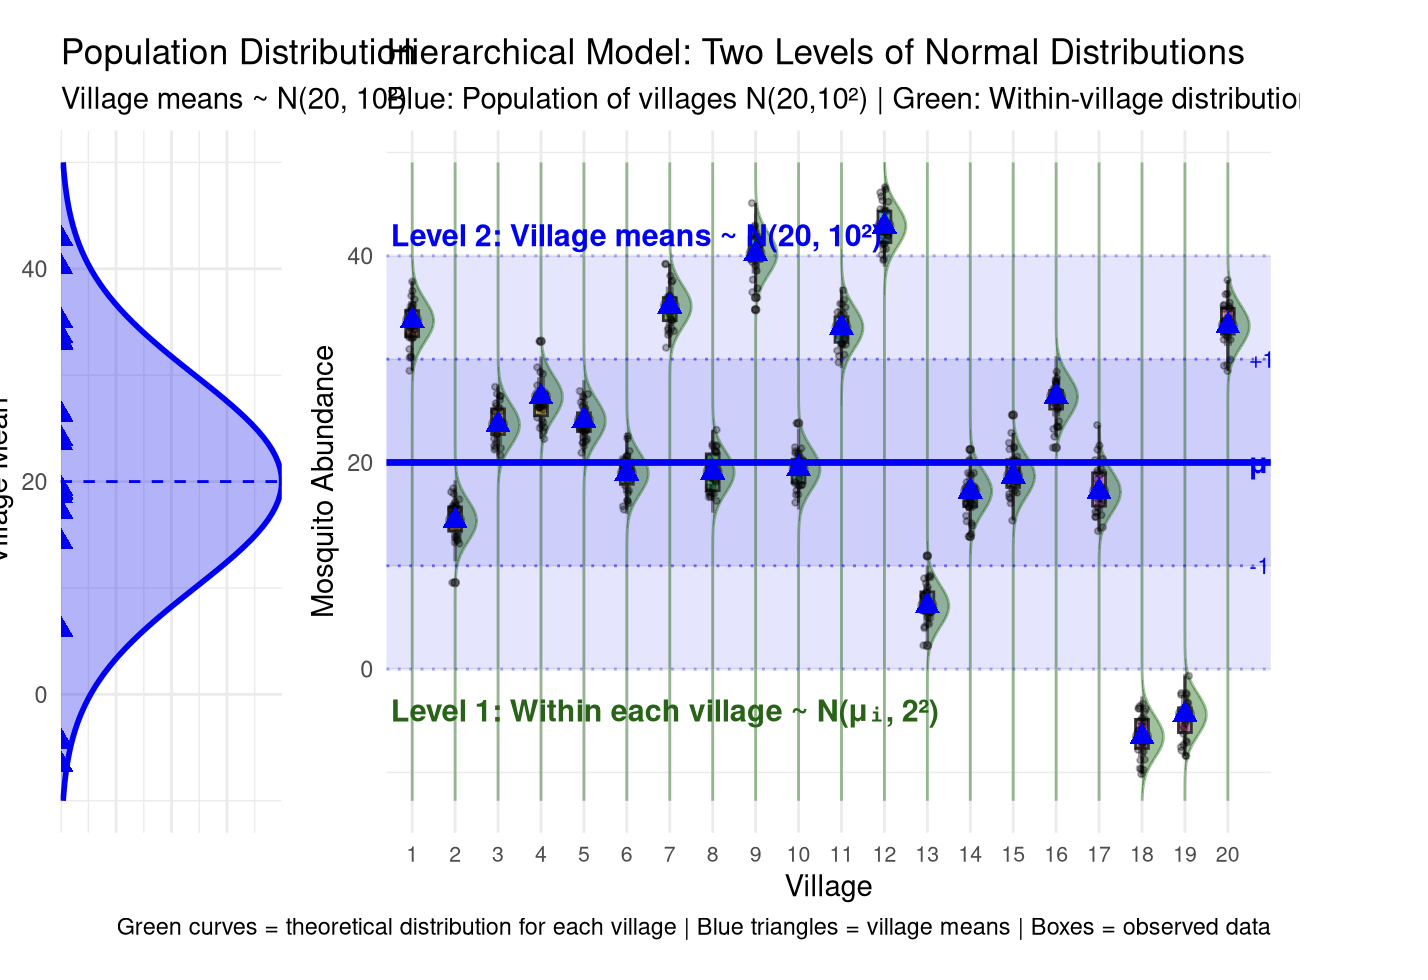
\includegraphics[width=1\linewidth]{overviews//general-cheatsheet/image.png}
\end{figure}

[Computational Advantages]
The mixed model representation allows:
\begin{enumerate}
    \item Use of standard LMM software
    \item Automatic selection of smoothing parameters via REML
    \item Proper uncertainty quantification including smoothing parameter uncertainty
    \item Natural handling of crossed and nested random effects
\end{enumerate}


\section{Generalized Linear Mixed Models (GLMMs)}

\subsection{Model Framework}

\subsubsection{Conditional Model}

\begin{definition}[GLMM Specification]
A GLMM specifies the distribution of $Y_{ij}$ conditional on random effects:
\begin{align}
Y_{ij}|\mathbf{u}_j &\sim \text{ExpFamily}(\mu_{ij}, \phi) \\
g(\mu_{ij}) &= g(E[Y_{ij}|\mathbf{u}_j]) = \mathbf{x}_{ij}^T\boldsymbol{\beta} + \mathbf{z}_{ij}^T\mathbf{u}_j \\
\mathbf{u}_j &\sim \mathcal{N}(\mathbf{0}, \mathbf{G})
\end{align}
where:
\begin{itemize}
    \item $g(\cdot)$ = link function
    \item $\mathbf{x}_{ij}$ = fixed effects covariates
    \item $\mathbf{z}_{ij}$ = random effects covariates
    \item $\mathbf{u}_j$ = random effects for cluster $j$
\end{itemize}
\end{definition}

\paragraph*{Key Distinction from LMM}
Unlike LMMs where we add random effects to the response, in GLMMs we add random effects to the \textbf{linear predictor} (on the link scale):
\begin{itemize}
    \item LMM: $Y_{ij} = \mathbf{x}_{ij}^T\boldsymbol{\beta} + \mathbf{z}_{ij}^T\mathbf{u}_j + \epsilon_{ij}$
    \item GLMM: $g(\mu_{ij}) = \mathbf{x}_{ij}^T\boldsymbol{\beta} + \mathbf{z}_{ij}^T\mathbf{u}_j$
\end{itemize}


\subsubsection{Marginal Likelihood}

\begin{theorem}[Marginal Likelihood]
The marginal likelihood requires integrating over the random effects:
\begin{equation}
L(\boldsymbol{\beta}, \boldsymbol{\theta}) = \prod_{j=1}^J \int \prod_{i=1}^{n_j} f(y_{ij}|\mathbf{u}_j, \boldsymbol{\beta}) \phi(\mathbf{u}_j; \mathbf{G}) d\mathbf{u}_j
\end{equation}
where:
\begin{itemize}
    \item $f(y_{ij}|\mathbf{u}_j, \boldsymbol{\beta})$ = conditional density from exponential family
    \item $\phi(\mathbf{u}_j; \mathbf{G})$ = multivariate normal density of random effects
\end{itemize}
\end{theorem}

\paragraph*{Computational Challenge}
This integral generally has no closed form except when:
\begin{enumerate}
    \item Linear model with normal errors (reduces to LMM)
    \item Binary data with probit link and normal random effects
\end{enumerate}
For other cases, we need approximation methods.

\subsection{Estimation Approaches}

\begin{remark}[The Fundamental Challenge]
In GLMMs, we need to evaluate:
\begin{equation}
L(\boldsymbol{\beta}, \boldsymbol{\theta}) = \prod_{j=1}^J \int \prod_{i=1}^{n_j} f(y_{ij}|\mathbf{u}_j, \boldsymbol{\beta}) \phi(\mathbf{u}_j; \mathbf{G}) d\mathbf{u}_j
\end{equation}
This integral is analytically intractable except for:
\begin{itemize}
    \item Normal-Normal: LMM (closed form)
    \item Binary-Probit: Probit model with normal random effects (reduces to normal integral)
\end{itemize}
We'll explore three approximation strategies.
\end{remark}

\subsubsection{Penalized Quasi-Likelihood (PQL)}

\begin{definition}[Core Idea of PQL]
PQL uses a first-order Taylor expansion to linearize the GLMM around current estimates, then fits the resulting LMM. It's "quasi" because it doesn't maximize a true likelihood.
\end{definition}

\begin{example}[PQL Derivation for Logistic-Normal Model]
Consider a random intercept logistic model:
\begin{align}
Y_{ij}|u_j &\sim \text{Bernoulli}(\pi_{ij}) \\
\text{logit}(\pi_{ij}) &= \beta_0 + \beta_1 x_{ij} + u_j \\
u_j &\sim \mathcal{N}(0, \tau^2)
\end{align}

\textbf{Step 1: Taylor expansion around current estimate}
Let $\eta_{ij}^* = \beta_0 + \beta_1 x_{ij} + u_j^*$ be the current linear predictor. Taylor expand:
\begin{align}
y_{ij} &\approx \pi_{ij}^* + \frac{\partial \pi_{ij}}{\partial \eta_{ij}}\bigg|_{\eta_{ij}^*} (\eta_{ij} - \eta_{ij}^*) \\
&= \pi_{ij}^* + \pi_{ij}^*(1-\pi_{ij}^*)(\eta_{ij} - \eta_{ij}^*)
\end{align}

Rearranging:
\begin{equation}
\underbrace{\eta_{ij}^* + \frac{y_{ij} - \pi_{ij}^*}{\pi_{ij}^*(1-\pi_{ij}^*)}}_{\tilde{y}_{ij} \text{ (working response)}} = \eta_{ij} + \underbrace{\frac{y_{ij} - \pi_{ij} - \pi_{ij}^*(1-\pi_{ij}^*)(\eta_{ij} - \eta_{ij}^*)}{\pi_{ij}^*(1-\pi_{ij}^*)}}_{\text{error term}}
\end{equation}

\textbf{Step 2: Working linear mixed model}
This suggests the LMM:
\begin{equation}
\tilde{y}_{ij} = \beta_0 + \beta_1 x_{ij} + u_j + e_{ij}
\end{equation}
with weights $w_{ij} = \pi_{ij}^*(1-\pi_{ij}^*)$ and $\text{Var}[e_{ij}] = 1/w_{ij}$.
\end{example}

\begin{definition}[General PQL Algorithm]
\textbf{Initialize}: $\boldsymbol{\beta}^{(0)}$, $\mathbf{u}^{(0)} = \mathbf{0}$, $\boldsymbol{\theta}^{(0)}$

\textbf{Iterate} until convergence:
\begin{enumerate}
    \item \textbf{Compute} current values:
    \begin{align}
    \eta_{ij}^{(t)} &= \mathbf{x}_{ij}^T\boldsymbol{\beta}^{(t)} + \mathbf{z}_{ij}^T\mathbf{u}_j^{(t)} \\
    \mu_{ij}^{(t)} &= g^{-1}(\eta_{ij}^{(t)})
    \end{align}
    
    \item \textbf{Create} working data:
    \begin{align}
    \tilde{y}_{ij}^{(t)} &= \eta_{ij}^{(t)} + (y_{ij} - \mu_{ij}^{(t)})\left[\frac{dg}{d\mu}\bigg|_{\mu_{ij}^{(t)}}\right] \\
    w_{ij}^{(t)} &= \left[\frac{d\mu}{d\eta}\bigg|_{\eta_{ij}^{(t)}}\right]^2 / V(\mu_{ij}^{(t)})
    \end{align}
    
    \item \textbf{Fit} weighted LMM:
    \begin{equation}
    \tilde{y}_{ij}^{(t)} = \mathbf{x}_{ij}^T\boldsymbol{\beta} + \mathbf{z}_{ij}^T\mathbf{u}_j + e_{ij}, \quad e_{ij} \sim \mathcal{N}(0, \sigma^2/w_{ij}^{(t)})
    \end{equation}
    to obtain $\boldsymbol{\beta}^{(t+1)}$, $\mathbf{u}^{(t+1)}$, $\boldsymbol{\theta}^{(t+1)}$
\end{enumerate}
\end{definition}

\begin{theorem}[PQL as Penalized Quasi-Score]
PQL approximately solves:
\begin{align}
\begin{pmatrix} \mathbf{0} \\ \mathbf{0} \end{pmatrix} &\approx 
\begin{pmatrix}
\sum_{i,j} \mathbf{x}_{ij}\frac{(y_{ij} - \mu_{ij})}{V(\mu_{ij})}h'(\eta_{ij}) \\
\sum_{i,j} \mathbf{z}_{ij}\frac{(y_{ij} - \mu_{ij})}{V(\mu_{ij})}h'(\eta_{ij}) - \mathbf{G}^{-1}\mathbf{u}
\end{pmatrix}
\end{align}
where $h = g^{-1}$ is the inverse link.
\end{theorem}

\begin{remark}[Critical Issues with PQL]
\begin{enumerate}
    \item \textbf{No true likelihood}: Cannot compute AIC/BIC reliably
    \item \textbf{Bias in variance components}:
    \begin{itemize}
        \item Binary data: Can underestimate $\tau^2$ by 50\% or more
        \item Count data: Less severe but still biased downward
        \item Bias increases as $\tau^2$ increases
    \end{itemize}
    \item \textbf{Poor for model selection}: Different fixed effects $\rightarrow$ different quasi-likelihoods
    \item \textbf{Inference issues}: Standard errors can be too small
\end{enumerate}
\end{remark}

\subsubsection{Laplace Approximation}

\begin{definition}[Laplace Principle]
The Laplace approximation uses:
\begin{equation}
\int e^{n h(x)} dx \approx \sqrt{\frac{2\pi}{n}} |h''(\hat{x})|^{-1/2} e^{n h(\hat{x})}
\end{equation}
where $\hat{x}$ maximizes $h(x)$. For GLMMs, we apply this to each integral over $\mathbf{u}_j$.
\end{definition}

\begin{example}[Worked Example: Binary Data]
For the logistic-normal model, we need:
\begin{equation}
\int \prod_{i=1}^{n_j} \frac{\exp(y_{ij}\eta_{ij})}{1 + \exp(\eta_{ij})} \cdot \frac{1}{\sqrt{2\pi\tau^2}}\exp\left(-\frac{u_j^2}{2\tau^2}\right) du_j
\end{equation}

Define the log-integrand:
\begin{equation}
h_j(u_j) = \sum_{i=1}^{n_j} [y_{ij}(\beta_0 + \beta_1 x_{ij} + u_j) - \log(1 + \exp(\beta_0 + \beta_1 x_{ij} + u_j))] - \frac{u_j^2}{2\tau^2}
\end{equation}

\textbf{Step 1}: Find mode $\hat{u}_j$ by solving:
\begin{equation}
\frac{\partial h_j}{\partial u_j} = \sum_{i=1}^{n_j} (y_{ij} - \pi_{ij}) - \frac{u_j}{\tau^2} = 0
\end{equation}

\textbf{Step 2}: Compute Hessian:
\begin{equation}
H_j = -\frac{\partial^2 h_j}{\partial u_j^2} = \sum_{i=1}^{n_j} \pi_{ij}(1-\pi_{ij}) + \frac{1}{\tau^2}
\end{equation}

\textbf{Step 3}: Approximate integral:
\begin{equation}
\int e^{h_j(u_j)} du_j \approx \sqrt{2\pi H_j^{-1}} \exp(h_j(\hat{u}_j))
\end{equation}
\end{example}

\begin{theorem}[General Laplace for GLMMs]
The Laplace-approximated log-likelihood is:
\begin{align}
\ell_{LA}(\boldsymbol{\beta}, \boldsymbol{\theta}) = \sum_{j=1}^J \Bigg[&\sum_{i=1}^{n_j} \log f(y_{ij}|\hat{\mathbf{u}}_j, \boldsymbol{\beta}) - \frac{1}{2}\hat{\mathbf{u}}_j^T\mathbf{G}^{-1}\hat{\mathbf{u}}_j \\
&- \frac{1}{2}\log|\mathbf{G}| - \frac{1}{2}\log|\mathbf{H}_j| \Bigg]
\end{align}
where $\mathbf{H}_j = -\frac{\partial^2}{\partial \mathbf{u}_j \partial \mathbf{u}_j^T}[\log f(\mathbf{y}_j|\mathbf{u}_j) - \frac{1}{2}\mathbf{u}_j^T\mathbf{G}^{-1}\mathbf{u}_j]|_{\hat{\mathbf{u}}_j}$
\end{theorem}

\begin{remark}[Properties of Laplace]
\begin{enumerate}
    \item \textbf{True (approximate) likelihood}: Can use for AIC/BIC
    \item \textbf{Accuracy}: $O(n_j^{-1})$ error for each cluster
    \item \textbf{Better than PQL}: Especially for binary data
    \item \textbf{Still biased}: Underestimates variance components (less than PQL)
\end{enumerate}
\end{remark}

\subsubsection{Adaptive Gauss-Hermite Quadrature}

\begin{definition}[Gaussian Quadrature Principle]
For integrals of the form $\int_{-\infty}^{\infty} f(x)e^{-x^2}dx$, we have exact equality:
\begin{equation}
\int_{-\infty}^{\infty} p_{2K-1}(x)e^{-x^2}dx = \sum_{k=1}^K w_k p_{2K-1}(x_k)
\end{equation}
for any polynomial $p_{2K-1}$ of degree $\leq 2K-1$.
\end{definition}

\begin{example}[AGHQ for Random Intercept]
Transform the integral for cluster $j$:
\begin{align}
I_j &= \int \prod_{i=1}^{n_j} f(y_{ij}|\beta_0 + \beta_1 x_{ij} + u_j) \phi(u_j; 0, \tau^2) du_j \\
&= \int \exp[h_j(u_j)] du_j
\end{align}

\textbf{Adaptive transformation}: Let $u_j = \hat{u}_j + \sqrt{2H_j^{-1}} z$ where:
\begin{itemize}
    \item $\hat{u}_j$ = mode of $h_j(u_j)$
    \item $H_j$ = negative second derivative at mode
\end{itemize}

Then:
\begin{equation}
I_j \approx \sqrt{2\pi H_j^{-1}} \sum_{k=1}^K w_k \exp[h_j(\hat{u}_j + \sqrt{2H_j^{-1}} z_k) + z_k^2]
\end{equation}
\end{example}

\begin{theorem}[Error Analysis]
For $K$ quadrature points:
\begin{itemize}
    \item Laplace ($K=1$): Error $= O(n_j^{-1})$
    \item AGHQ ($K>1$): Error $= O(n_j^{-K})$ for well-behaved integrands
    \item Practical: $K=7-9$ often indistinguishable from "exact"
\end{itemize}
\end{theorem}

\begin{remark}[Method Comparison for Model Selection]
\begin{center}
\begin{tabular}{|l|c|c|c|c|}
\hline
\textbf{Method} & \textbf{True LL} & \textbf{AIC/BIC} & \textbf{Var Comp Bias} & \textbf{Speed} \\
\hline
PQL & No & Unreliable & High (binary) & Fast \\
Laplace & Approximate & Good & Moderate & Medium \\
AGHQ (K=7) & Near-exact & Excellent & Minimal & Slow \\
AGHQ (K=20) & "Exact" & Excellent & Negligible & Very slow \\
\hline
\end{tabular}
\end{center}
\end{remark}

\begin{example}[When Methods Fail]
Consider binary data with:
\begin{itemize}
    \item 30 clusters, 5 observations per cluster
    \item True $\tau^2 = 4$ (large random effects)
    \item 50\% response rate
\end{itemize}

Results:
\begin{itemize}
    \item \textbf{PQL}: $\hat{\tau}^2 \approx 2.0$ (50\% underestimate)
    \item \textbf{Laplace}: $\hat{\tau}^2 \approx 3.2$ (20\% underestimate)
    \item \textbf{AGHQ(7)}: $\hat{\tau}^2 \approx 3.9$ (2.5\% underestimate)
\end{itemize}

For AIC-based model selection between models with/without a covariate:
\begin{itemize}
    \item PQL: Wrong model selected 40\% of time
    \item Laplace: Wrong model selected 15\% of time
    \item AGHQ(7): Wrong model selected 5\% of time
\end{itemize}
\end{example}

\begin{remark}[Practical Recommendations]
\begin{enumerate}
    \item \textbf{Use PQL only for}: Initial values, very large datasets, or when bias is acceptable
    \item \textbf{Use Laplace for}: Routine analysis with moderate cluster sizes
    \item \textbf{Use AGHQ for}: 
    \begin{itemize}
        \item Publication/final results
        \item Model selection via AIC/BIC
        \item Small clusters or large variance components
        \item When computational time is not critical
    \end{itemize}
    \item \textbf{For binary data}: Never trust PQL for inference
    \item \textbf{Check convergence}: Compare Laplace vs AGHQ(7) estimates
\end{enumerate}
\end{remark}

\subsection{Marginal Effects in GLMMs}

\subsubsection{Subject-Specific Effects}

\begin{definition}[Conditional Marginal Effect]
The marginal effect conditional on random effects is:
\begin{equation}
\frac{\partial E[Y_{ij}|\mathbf{u}_j]}{\partial x_{ijk}} = \frac{\partial \mu_{ij}}{\partial x_{ijk}} = g'^{-1}(\eta_{ij}) \cdot \beta_k
\end{equation}
This varies by:
\begin{itemize}
    \item Individual characteristics ($\mathbf{x}_{ij}$)
    \item Cluster-specific effects ($\mathbf{u}_j$)
\end{itemize}
\end{definition}

\paragraph*{Logistic GLMM}
For binary outcomes with random intercept:
\begin{align}
\text{logit}(\pi_{ij}) &= \beta_0 + \beta_1 x_{ij} + u_j \\
\frac{\partial \pi_{ij}}{\partial x_{ij}} &= \pi_{ij}(1-\pi_{ij})\beta_1
\end{align}
where $\pi_{ij} = \frac{\exp(\beta_0 + \beta_1 x_{ij} + u_j)}{1 + \exp(\beta_0 + \beta_1 x_{ij} + u_j)}$ depends on $u_j$.


\subsubsection{Population-Average Effects}

\begin{definition}[Marginal Effect]
The population-average marginal effect integrates over random effects:
\begin{equation}
\frac{\partial E[Y_{ij}]}{\partial x_{ijk}} = \int \frac{\partial E[Y_{ij}|\mathbf{u}_j]}{\partial x_{ijk}} \phi(\mathbf{u}_j)d\mathbf{u}_j
\end{equation}
\end{definition}

\begin{theorem}[Approximation Methods]
\begin{enumerate}
    \item \textbf{Monte Carlo}: 
    \begin{equation}
    \frac{\partial E[Y_{ij}]}{\partial x_{ijk}} \approx \frac{1}{M}\sum_{m=1}^M g'^{-1}(\mathbf{x}_{ij}^T\boldsymbol{\beta} + \mathbf{z}_{ij}^T\mathbf{u}_j^{(m)})\beta_k
    \end{equation}
    where $\mathbf{u}_j^{(m)} \sim \mathcal{N}(\mathbf{0}, \mathbf{G})$
    
    \item \textbf{Delta method}: For small $\text{Var}[\mathbf{u}_j]$
    \item \textbf{Numerical integration}: Using quadrature
\end{enumerate}
\end{theorem}

\paragraph*{SS vs PA Interpretation}
\begin{itemize}
    \item \textbf{Subject-specific (SS)}: Effect for a specific cluster
    \item \textbf{Population-average (PA)}: Average effect across all clusters
    \item For linear models: SS = PA
    \item For nonlinear models: Generally PA < SS (attenuation)
\end{itemize}


\subsection{Polynomial and Nonlinear Effects in GLMMs}

\subsubsection{Polynomial GLMMs}

\paragraph{Model Specification}

\begin{definition}[Polynomial GLMM]
\begin{equation}
g(E[Y_{ij}|\mathbf{u}_j]) = \beta_0 + \beta_1 x_{ij} + \beta_2 x_{ij}^2 + \cdots + \beta_p x_{ij}^p + \mathbf{z}_{ij}^T\mathbf{u}_j
\end{equation}
Common specifications:
\begin{itemize}
    \item Random intercept only: $\mathbf{z}_{ij}^T\mathbf{u}_j = u_{0j}$
    \item Random polynomial: $\mathbf{z}_{ij}^T\mathbf{u}_j = u_{0j} + u_{1j}x_{ij} + u_{2j}x_{ij}^2$
\end{itemize}
\end{definition}

\paragraph{Marginal Effects in Polynomial GLMMs}

\begin{theorem}[Subject-Specific Marginal Effect]
\begin{equation}
\frac{\partial E[Y_{ij}|\mathbf{u}_j]}{\partial x_{ij}} = g'^{-1}(\eta_{ij})\left(\beta_1 + 2\beta_2 x_{ij} + \cdots + p\beta_p x_{ij}^{p-1} + u_{1j} + 2u_{2j}x_{ij}\right)
\end{equation}
if random slopes are included.
\end{theorem}

\subsubsection{Generalized Additive Mixed Models (GAMMs)}

\paragraph{Model Framework}

\begin{definition}[GAMM]
\begin{equation}
g(E[Y_{ij}|\mathbf{u}_j]) = f_1(x_{1ij}) + f_2(x_{2ij}) + \cdots + f_p(x_{pij}) + \mathbf{z}_{ij}^T\mathbf{u}_j
\end{equation}
where $f_k$ are smooth functions.
\end{definition}

\paragraph{Double Penalization}

\paragraph*{Two Types of Penalties}
GAMMs involve:
\begin{enumerate}
    \item \textbf{Smoothness penalties}: $\lambda_k \int [f_k''(x)]^2dx$ for each smooth
    \item \textbf{Random effects penalty}: $\mathbf{u}^T\mathbf{G}^{-1}\mathbf{u}$
\end{enumerate}
Both can be handled in a unified framework by treating smooths as random effects.


\subsubsection{Hierarchical Curves}

\paragraph{Population and Subject-Specific Curves}

\begin{definition}[Hierarchical Curve Model]
\begin{align}
g(E[Y_{ij}|\mathbf{u}_j]) &= f_{pop}(x_{ij}) + f_j(x_{ij}) \\
&= \sum_{k=1}^K \beta_k b_k(x_{ij}) + \sum_{k=1}^K u_{jk} b_k(x_{ij}) \nonumber
\end{align}
where:
\begin{itemize}
    \item $f_{pop}(x)$ = population-average curve (fixed)
    \item $f_j(x)$ = cluster-specific deviation (random)
    \item Same basis functions $\{b_k\}$ for both
\end{itemize}
\end{definition}

\begin{proposition}[Interpretation]
\begin{itemize}
    \item Total curve for cluster $j$: $f_{total,j}(x) = f_{pop}(x) + f_j(x)$
    \item Between-cluster variance function: $\text{Var}[f_j(x)] = \mathbf{b}(x)^T\mathbf{G}\mathbf{b}(x)$
    \item Pointwise confidence bands incorporate both fixed and random uncertainty
\end{itemize}
\end{proposition}

\section{Model Diagnostics and Inference}

\subsection{Residual Analysis}

\subsubsection{Types of Residuals}

\begin{definition}[Residuals in Mixed Models]
For mixed models, we distinguish between residuals at different levels:
\begin{align}
\text{Marginal residuals}: & \quad \mathbf{r}_m = \mathbf{y} - \mathbf{X}\hat{\boldsymbol{\beta}} \\
\text{Conditional residuals}: & \quad \mathbf{r}_c = \mathbf{y} - \mathbf{X}\hat{\boldsymbol{\beta}} - \mathbf{Z}\hat{\mathbf{u}} \\
\text{Random effects}: & \quad \hat{\mathbf{u}} \text{ (predictions of random deviations)}
\end{align}
\end{definition}

\begin{theorem}[Properties of Residuals]
Under the correct model:
\begin{align}
E[\mathbf{r}_m] &= \mathbf{0}, \quad \text{Var}[\mathbf{r}_m] = \mathbf{V} - \mathbf{X}(\mathbf{X}^T\mathbf{V}^{-1}\mathbf{X})^{-1}\mathbf{X}^T \\
E[\mathbf{r}_c] &= \mathbf{0}, \quad \text{Var}[\mathbf{r}_c] = \mathbf{R} - \mathbf{Q}
\end{align}
where $\mathbf{Q}$ accounts for uncertainty in predicting $\mathbf{u}$.
\end{theorem}

\begin{definition}[Standardized Residuals]
To account for heterogeneous variances:
\begin{align}
\text{Standardized marginal}: & \quad r_{m,i}^{std} = \frac{r_{m,i}}{\sqrt{\hat{V}_{ii}(1-h_{ii})}} \\
\text{Standardized conditional}: & \quad r_{c,i}^{std} = \frac{r_{c,i}}{\hat{\sigma}\sqrt{1-h_{ii}^*}}
\end{align}
where $h_{ii}$ and $h_{ii}^*$ are leverage values from marginal and conditional models.
\end{definition}

\begin{remark}[Interpretation of Different Residuals]
\begin{itemize}
    \item \textbf{Marginal residuals}: Check overall model fit, detect systematic patterns
    \item \textbf{Conditional residuals}: Check within-cluster assumptions, homoscedasticity
    \item \textbf{Random effects}: Check normality assumption, identify outlying clusters
\end{itemize}
\end{remark}

\begin{definition}[Residuals for GLMMs]
For GLMMs, we additionally have:
\begin{align}
\text{Pearson residuals}: & \quad r_{P,ij} = \frac{y_{ij} - \hat{\mu}_{ij}}{\sqrt{V(\hat{\mu}_{ij})}} \\
\text{Deviance residuals}: & \quad r_{D,ij} = \text{sign}(y_{ij} - \hat{\mu}_{ij})\sqrt{2[l(y_{ij};y_{ij}) - l(y_{ij};\hat{\mu}_{ij})]}
\end{align}
where $l(y;\mu)$ is the log-likelihood contribution.
\end{definition}

\subsubsection{Diagnostic Plots}

\begin{proposition}[Key Diagnostic Plots]
\begin{enumerate}
    \item \textbf{Residuals vs Fitted}: 
    \begin{itemize}
        \item Plot $r_{c,i}^{std}$ vs $\hat{y}_i$ for LMMs
        \item Plot Pearson residuals vs $\hat{\eta}_i$ for GLMMs
        \item Check for: patterns, heteroscedasticity
    \end{itemize}
    
    \item \textbf{Q-Q Plots}:
    \begin{itemize}
        \item Conditional residuals: $r_{c,i}^{std}$ vs normal quantiles
        \item Random effects: $\hat{u}_j$ vs normal quantiles for each level
        \item Check for: normality, outliers
    \end{itemize}
    
    \item \textbf{Scale-Location Plot}:
    \begin{itemize}
        \item Plot $\sqrt{|r_{c,i}^{std}|}$ vs fitted values
        \item Check for: heteroscedasticity patterns
    \end{itemize}
    
    \item \textbf{Cluster-Level Diagnostics}:
    \begin{itemize}
        \item Caterpillar plots of $\hat{u}_j$ with confidence intervals
        \item Check for: outlying clusters, shrinkage patterns
    \end{itemize}
\end{enumerate}
\end{proposition}

\subsection{Hypothesis Testing}

\subsubsection{Wald Tests}

\begin{definition}[Wald Test Statistic]
For testing $H_0: \mathbf{L}\boldsymbol{\beta} = \mathbf{c}$ where $\mathbf{L}$ is $r \times p$:
\begin{equation}
W = (\mathbf{L}\hat{\boldsymbol{\beta}} - \mathbf{c})^T[\mathbf{L}\hat{\mathbf{V}}_{\beta}\mathbf{L}^T]^{-1}(\mathbf{L}\hat{\boldsymbol{\beta}} - \mathbf{c})
\end{equation}
where $\hat{\mathbf{V}}_{\beta} = (\mathbf{X}^T\hat{\mathbf{V}}^{-1}\mathbf{X})^{-1}$.
\end{definition}

\begin{theorem}[Asymptotic Distribution]
Under $H_0$ and regularity conditions:
\begin{equation}
W \xrightarrow{d} \chi^2_r
\end{equation}
For finite samples with LMMs, an F-approximation is often used:
\begin{equation}
F = W/r \sim F_{r,\nu}
\end{equation}
where $\nu$ = approximate denominator degrees of freedom.
\end{theorem}

\begin{remark}[Degrees of Freedom Approximations]
Several methods exist for $\nu$:
\begin{itemize}
    \item \textbf{Containment}: $\nu = n_{\text{lowest}} - p_{\text{lowest}}$
    \item \textbf{Satterthwaite}: Complex function of variance components
    \item \textbf{Kenward-Roger}: Includes finite-sample corrections
\end{itemize}
\end{remark}

\subsubsection{Likelihood Ratio Tests}

\begin{definition}[LRT for Nested Models]
For models $M_0 \subset M_1$:
\begin{equation}
LRT = -2[\ell_0 - \ell_1] = -2\log\left(\frac{L_0}{L_1}\right)
\end{equation}
\end{definition}

\begin{theorem}[LRT Distribution]
\textbf{Case 1: Testing fixed effects (same variance structure)}
\begin{equation}
LRT \xrightarrow{d} \chi^2_{df}
\end{equation}
where $df = \dim(\boldsymbol{\beta}_1) - \dim(\boldsymbol{\beta}_0)$.

\textbf{Case 2: Testing variance components}
The distribution is a mixture of $\chi^2$ distributions when testing on the boundary (e.g., $H_0: \tau^2 = 0$).
\end{theorem}

\begin{remark}[Boundary Issues]
When testing $H_0: \tau^2 = 0$:
\begin{itemize}
    \item The null hypothesis is on the boundary of parameter space
    \item Standard $\chi^2$ theory doesn't apply
    \item Distribution is typically $0.5\chi^2_0 + 0.5\chi^2_1$ (50:50 mixture)
    \item Conservative approach: Use $\chi^2_1$ (gives larger p-values)
\end{itemize}
\end{remark}

\begin{proposition}[REML vs ML for LRT]
\begin{itemize}
    \item \textbf{Testing fixed effects}: Must use ML (not REML)
    \item \textbf{Testing variance components}: Can use REML if fixed effects are same
    \item \textbf{Model comparison}: Only valid when models are nested
\end{itemize}
\end{proposition}

\subsubsection{Parametric Bootstrap Tests}

\begin{definition}[Parametric Bootstrap for Mixed Models]
\begin{enumerate}
    \item Fit model under $H_0$: obtain $\hat{\boldsymbol{\beta}}_0$, $\hat{\boldsymbol{\theta}}_0$
    \item For $b = 1, \ldots, B$:
    \begin{enumerate}
        \item Generate $\mathbf{u}^{(b)} \sim \mathcal{N}(\mathbf{0}, \hat{\mathbf{G}}_0)$
        \item Generate $\mathbf{y}^{(b)} = \mathbf{X}\hat{\boldsymbol{\beta}}_0 + \mathbf{Z}\mathbf{u}^{(b)} + \boldsymbol{\epsilon}^{(b)}$
        \item Fit both models to $\mathbf{y}^{(b)}$, compute $LRT^{(b)}$
    \end{enumerate}
    \item P-value $= \frac{1}{B}\sum_{b=1}^B I(LRT^{(b)} \geq LRT_{obs})$
\end{enumerate}
\end{definition}

\begin{remark}[When to Use Bootstrap]
Bootstrap is particularly useful for:
\begin{itemize}
    \item Small samples
    \item Testing variance components
    \item Non-standard hypotheses
    \item When asymptotic theory is questionable
\end{itemize}
\end{remark}

\subsection{Model Selection}

\begin{definition}[Information Criteria]
For model with likelihood $L$ and $p$ parameters:
\begin{align}
\text{AIC} &= -2\log L + 2p \\
\text{BIC} &= -2\log L + p\log(n) \\
\text{cAIC} &= -2\log L + 2p + \frac{2p(p+1)}{n-p-1}
\end{align}
\end{definition}

\begin{remark}[Counting Parameters in Mixed Models]
For mixed models, $p$ includes:
\begin{itemize}
    \item All fixed effects parameters
    \item All variance components (including covariances)
    \item For AIC: Some debate about counting variance components
    \item Conservative: Count all parameters
\end{itemize}
\end{remark}

\begin{definition}[Conditional AIC]
For mixed models, Vaida and Blanchard (2005) propose:
\begin{equation}
\text{cAIC} = -2\log L(\hat{\boldsymbol{\beta}}, \hat{\boldsymbol{\theta}}|\mathbf{y}) + 2\rho
\end{equation}
where $\rho = \text{tr}(\mathbf{H})$ is the effective degrees of freedom, with $\mathbf{H}$ the hat matrix from the marginal model.
\end{definition}

\begin{theorem}[Model Selection Guidelines]
\begin{itemize}
    \item \textbf{AIC}: Selects model with best predictive performance
    \item \textbf{BIC}: Selects "true" model (if it exists) as $n \to \infty$
    \item \textbf{Difference of 2}: Weak evidence for better model
    \item \textbf{Difference of 5-10}: Strong evidence
    \item \textbf{Difference > 10}: Very strong evidence
\end{itemize}
\end{theorem}

\subsection{Inference for Variance Components}

\begin{proposition}[Challenges in Variance Component Inference]
\begin{enumerate}
    \item \textbf{Non-negative constraint}: $\tau^2 \geq 0$
    \item \textbf{Non-normal sampling distribution}: Especially for small clusters
    \item \textbf{Correlation with fixed effects}: Affects standard errors
\end{enumerate}
\end{proposition}

\begin{definition}[Profile Likelihood CI for Variance Components]
For parameter $\tau^2$:
\begin{enumerate}
    \item Define profile likelihood: $\ell_p(\tau^2) = \max_{\boldsymbol{\beta}} \ell(\boldsymbol{\beta}, \tau^2)$
    \item Find values where $-2[\ell_p(\tau^2) - \ell_p(\hat{\tau}^2)] = \chi^2_{1,1-\alpha}$
    \item These give $(1-\alpha)$ confidence interval
\end{enumerate}
\end{definition}

\begin{remark}[Bootstrap Confidence Intervals]
For variance components, bootstrap CIs often perform better:
\begin{itemize}
    \item \textbf{Percentile method}: Use quantiles of bootstrap distribution
    \item \textbf{BCa method}: Bias-corrected and accelerated
    \item \textbf{Parametric bootstrap}: Generally preferred for mixed models
\end{itemize}
\end{remark}

\subsection{Diagnostics for Model Assumptions}

\begin{theorem}[Testing Random Effects Distribution]
To test normality of random effects:
\begin{enumerate}
    \item \textbf{Formal tests}: Shapiro-Wilk on $\hat{\mathbf{u}}$
    \item \textbf{Graphical}: Q-Q plots by random effect level
    \item \textbf{Robust alternatives}: Consider t-distributed random effects
\end{enumerate}
\end{theorem}

\begin{definition}[Influence Diagnostics]
\textbf{Cook's Distance for clusters}:
\begin{equation}
D_j = \frac{(\hat{\boldsymbol{\beta}} - \hat{\boldsymbol{\beta}}_{(-j)})^T\mathbf{X}^T\mathbf{V}^{-1}\mathbf{X}(\hat{\boldsymbol{\beta}} - \hat{\boldsymbol{\beta}}_{(-j)})}{p}
\end{equation}
where $\hat{\boldsymbol{\beta}}_{(-j)}$ is the estimate without cluster $j$.
\end{definition}

\begin{remark}[Diagnostic Strategy]
\begin{enumerate}
    \item Check conditional residuals for within-cluster assumptions
    \item Check marginal residuals for overall model adequacy
    \item Examine random effects for distributional assumptions
    \item Use influence measures to identify influential clusters
    \item Consider robust methods if assumptions are violated
\end{enumerate}
\end{remark}

\subsection{Common Statistical Tests in Epidemiology}

\subsubsection{Tests for Regression Coefficients}

\begin{definition}[t-test for Individual Coefficients]
The most common test for regression coefficients tests $H_0: \beta_j = 0$:
\begin{equation}
t = \frac{\hat{\beta}_j - 0}{\text{SE}(\hat{\beta}_j)} = \frac{\hat{\beta}_j}{\sqrt{\hat{\sigma}^2[(\mathbf{X}^T\mathbf{X})^{-1}]_{jj}}}
\end{equation}
Under $H_0$: $t \sim t_{n-p}$ (Student's t-distribution).
\end{definition}

\begin{remark}[Interpretation in Epidemiology]
\begin{itemize}
    \item \textbf{Linear regression}: Tests if exposure has any linear association with outcome
    \item \textbf{Logistic regression}: Tests if exposure affects log-odds (OR $\neq$ 1)
    \item \textbf{Cox regression}: Tests if exposure affects hazard (HR $\neq$ 1)
    \item P-value: Probability of seeing this strong an association by chance alone
\end{itemize}
\end{remark}

\begin{proposition}[Relationship to Confidence Intervals]
The t-test is equivalent to checking if the $(1-\alpha)$ CI excludes 0:
\begin{equation}
\text{CI}: \hat{\beta}_j \pm t_{n-p,1-\alpha/2} \cdot \text{SE}(\hat{\beta}_j)
\end{equation}
\begin{itemize}
    \item If CI excludes 0 $\Leftrightarrow$ $|t| > t_{n-p,1-\alpha/2}$ $\Leftrightarrow$ p-value $< \alpha$
    \item Width of CI indicates precision of estimate
\end{itemize}
\end{proposition}

\subsubsection{Chi-Square Tests}

\begin{definition}[Pearson's Chi-Square Test]
For a contingency table with observed counts $O_{ij}$ and expected counts $E_{ij}$:
\begin{equation}
\chi^2 = \sum_{i=1}^r \sum_{j=1}^c \frac{(O_{ij} - E_{ij})^2}{E_{ij}}
\end{equation}
Under $H_0$ (independence): $\chi^2 \sim \chi^2_{(r-1)(c-1)}$.
\end{definition}

\begin{example}[2×2 Table in Epidemiology]
For exposure-disease association:
\begin{center}
\begin{tabular}{|l|c|c|c|}
\hline
 & Disease & No Disease & Total \\
\hline
Exposed & $a$ & $b$ & $a+b$ \\
Not Exposed & $c$ & $d$ & $c+d$ \\
\hline
Total & $a+c$ & $b+d$ & $n$ \\
\hline
\end{tabular}
\end{center}

Expected counts under independence:
\begin{equation}
E_{11} = \frac{(a+b)(a+c)}{n}, \quad E_{12} = \frac{(a+b)(b+d)}{n}, \text{ etc.}
\end{equation}

Chi-square statistic:
\begin{equation}
\chi^2 = \frac{n(ad-bc)^2}{(a+b)(c+d)(a+c)(b+d)}
\end{equation}
\end{example}

\begin{remark}[Continuity Correction]
For 2×2 tables with small expected counts, Yates' correction:
\begin{equation}
\chi^2_{\text{Yates}} = \frac{n(|ad-bc| - n/2)^2}{(a+b)(c+d)(a+c)(b+d)}
\end{equation}
Use when any expected count $< 5$.
\end{remark}

\begin{theorem}[Relationship to Other Tests]
For 2×2 tables:
\begin{itemize}
    \item $\chi^2 = z^2$ where $z$ is from two-proportion z-test
    \item Equivalent to logistic regression with binary predictor
    \item Related to Fisher's exact test (uses $\chi^2$ distribution as approximation)
\end{itemize}
\end{theorem}

\subsubsection{Wilcoxon Rank-Sum and Mann-Whitney U Tests}

\begin{definition}[Wilcoxon Rank-Sum Test]
For two groups with sizes $n_1$ and $n_2$:
\begin{enumerate}
    \item Pool all observations and rank from 1 to $N = n_1 + n_2$
    \item Calculate $W_1 = \sum_{i \in \text{Group 1}} R_i$ (sum of ranks in group 1)
    \item Test statistic: $W = W_1$ or $W = \min(W_1, W_2)$
\end{enumerate}
\end{definition}

\begin{definition}[Mann-Whitney U Test]
Count the number of pairs $(X_i, Y_j)$ where $X_i < Y_j$:
\begin{equation}
U_1 = \sum_{i=1}^{n_1} \sum_{j=1}^{n_2} I(X_i < Y_j)
\end{equation}
where $X_i$ are observations from group 1, $Y_j$ from group 2.
\end{definition}

\begin{theorem}[Equivalence of Wilcoxon and Mann-Whitney]
The two tests are exactly equivalent:
\begin{equation}
U_1 = W_1 - \frac{n_1(n_1+1)}{2}
\end{equation}

\textbf{Intuitive explanation}:
\begin{itemize}
    \item $W_1$ = sum of ranks in group 1
    \item $\frac{n_1(n_1+1)}{2}$ = sum of ranks if group 1 had the $n_1$ smallest values
    \item $U_1$ = excess rank sum = number of "inversions"
    \item Both measure how much group 1 tends to have larger values than group 2
\end{itemize}
\end{theorem}

\begin{proof}[Intuitive Proof]
Consider the contribution to $W_1$ from each observation $X_i$:
\begin{itemize}
    \item Rank of $X_i$ = (number of $X$'s $\leq X_i$) + (number of $Y$'s $< X_i$)
    \item Sum over all $X_i$: $W_1 = \frac{n_1(n_1+1)}{2} + \sum_i \sum_j I(Y_j < X_i)$
    \item But $\sum_i \sum_j I(Y_j < X_i) = n_1 n_2 - U_1$
    \item Therefore: $U_1 = W_1 - \frac{n_1(n_1+1)}{2}$
\end{itemize}
\end{proof}

\begin{remark}[Interpretation]
\begin{itemize}
    \item \textbf{Null hypothesis}: $P(X > Y) = 0.5$ (stochastic equality)
    \item \textbf{Alternative}: $P(X > Y) \neq 0.5$ (location shift or more general)
    \item \textbf{Effect size}: $P(X > Y) = U_1/(n_1 n_2)$ (probability of superiority)
    \item \textbf{Not just medians}: Tests entire distribution shift
\end{itemize}
\end{remark}

\subsubsection{Normality Tests}

\begin{definition}[Shapiro-Wilk Test]
Tests $H_0$: data come from normal distribution
\begin{equation}
W = \frac{\left(\sum_{i=1}^n a_i x_{(i)}\right)^2}{\sum_{i=1}^n (x_i - \bar{x})^2}
\end{equation}
where:
\begin{itemize}
    \item $x_{(i)}$ = ordered statistics
    \item $a_i$ = coefficients from expected values of order statistics
    \item $W \approx 1$ suggests normality
\end{itemize}
\end{definition}

\begin{remark}[Limitations of Shapiro-Wilk]
\begin{enumerate}
    \item \textbf{Sample size sensitivity}:
    \begin{itemize}
        \item Small $n$: Low power, fails to detect non-normality
        \item Large $n$: Too sensitive, rejects for trivial deviations
    \end{itemize}
    \item \textbf{Multiple testing}: Testing many variables inflates Type I error
    \item \textbf{Not robust}: Sensitive to outliers
    \item \textbf{Limited information}: Only gives yes/no answer
\end{enumerate}
\end{remark}

\begin{definition}[Moments-Based Assessment]
Instead of formal tests, examine distributional characteristics:
\begin{align}
\text{Skewness} &= \frac{\frac{1}{n}\sum_{i=1}^n (x_i - \bar{x})^3}{\left[\frac{1}{n}\sum_{i=1}^n (x_i - \bar{x})^2\right]^{3/2}} \\
\text{Kurtosis} &= \frac{\frac{1}{n}\sum_{i=1}^n (x_i - \bar{x})^4}{\left[\frac{1}{n}\sum_{i=1}^n (x_i - \bar{x})^2\right]^2} - 3
\end{align}
\end{definition}

\begin{proposition}[Why Kurtosis Analysis is Often Better]
\begin{enumerate}
    \item \textbf{Quantitative information}:
    \begin{itemize}
        \item Skewness: Direction and degree of asymmetry
        \item Kurtosis: Tail heaviness (outlier proneness)
        \item Normal: Skewness = 0, Kurtosis = 0
    \end{itemize}
    
    \item \textbf{Robustness guidance}:
    \begin{itemize}
        \item $|\text{Skewness}| < 1$: Mild, most methods robust
        \item $|\text{Skewness}| > 2$: Severe, consider transformation
        \item $\text{Kurtosis} > 3$: Heavy tails, consider robust methods
    \end{itemize}
    
    \item \textbf{Sample size invariant}: Thresholds don't depend on $n$
    
    \item \textbf{Visual confirmation}: Combine with Q-Q plots
\end{enumerate}
\end{proposition}

\begin{remark}[Practical Recommendations for Normality]
\begin{enumerate}
    \item \textbf{Don't over-rely on tests}: Shapiro-Wilk $p < 0.05$ doesn't mean analysis fails
    \item \textbf{Consider context}:
    \begin{itemize}
        \item Linear regression: Residual normality matters, not variable normality
        \item t-tests: Robust to moderate non-normality if $n > 30$
        \item Mixed models: Random effects normality more important
    \end{itemize}
    \item \textbf{Use multiple approaches}:
    \begin{itemize}
        \item Visual: Q-Q plots, histograms
        \item Descriptive: Skewness, kurtosis
        \item Formal tests: As supplementary evidence only
    \end{itemize}
\end{enumerate}
\end{remark}

\subsubsection{Tests for Paired Data}

\begin{definition}[Paired t-test]
For paired observations $(X_i, Y_i)$, test on differences $D_i = X_i - Y_i$:
\begin{equation}
t = \frac{\bar{D} - 0}{s_D/\sqrt{n}} = \frac{\bar{D}\sqrt{n}}{s_D}
\end{equation}
where $s_D$ is the sample standard deviation of differences.
\end{definition}

\begin{definition}[Wilcoxon Signed-Rank Test]
Non-parametric alternative for paired data:
\begin{enumerate}
    \item Calculate $D_i = X_i - Y_i$ for each pair
    \item Rank $|D_i|$ from 1 to $n$
    \item Sum ranks for positive differences: $W^+ = \sum_{D_i > 0} R_i$
    \item Compare to null distribution
\end{enumerate}
\end{definition}

\begin{remark}[Choice Between Tests]
\begin{center}
\begin{tabular}{|l|l|l|}
\hline
\textbf{Scenario} & \textbf{Recommended Test} & \textbf{Reason} \\
\hline
Normal differences & Paired t-test & Most powerful \\
Symmetric, non-normal & Wilcoxon signed-rank & Robust, nearly as powerful \\
Skewed differences & Transform or Wilcoxon & t-test assumptions violated \\
Ordinal outcomes & Wilcoxon signed-rank & t-test inappropriate \\
\hline
\end{tabular}
\end{center}
\end{remark}

\subsubsection{Multiple Testing Corrections}

\begin{definition}[Family-Wise Error Rate (FWER)]
Probability of at least one Type I error among $m$ tests:
\begin{equation}
\text{FWER} = P(\text{at least one false positive}) = 1 - (1-\alpha)^m \approx m\alpha
\end{equation}
for independent tests.
\end{definition}

\begin{theorem}[Common Corrections]
\begin{enumerate}
    \item \textbf{Bonferroni}: Use $\alpha' = \alpha/m$ for each test
    \begin{itemize}
        \item Controls FWER $\leq \alpha$
        \item Conservative (especially for correlated tests)
    \end{itemize}
    
    \item \textbf{Holm-Bonferroni}: Sequential procedure
    \begin{itemize}
        \item Order p-values: $p_{(1)} \leq p_{(2)} \leq \cdots \leq p_{(m)}$
        \item Reject $H_{(i)}$ if $p_{(i)} \leq \alpha/(m-i+1)$
        \item More powerful than Bonferroni
    \end{itemize}
    
    \item \textbf{False Discovery Rate (FDR) - Benjamini-Hochberg}:
    \begin{itemize}
        \item Controls expected proportion of false positives
        \item Find largest $i$ such that $p_{(i)} \leq \frac{i}{m}\alpha$
        \item Reject $H_{(1)}, \ldots, H_{(i)}$
    \end{itemize}
\end{enumerate}
\end{theorem}

\begin{remark}[When to Use Each]
\begin{itemize}
    \item \textbf{Bonferroni}: Few tests ($m < 5$), critical decisions
    \item \textbf{Holm}: Moderate number of tests, need FWER control
    \item \textbf{FDR}: Many tests ($m > 20$), exploratory analysis
    \item \textbf{No correction}: Pre-specified primary outcome only
\end{itemize}
\end{remark}




\end{document}